\documentclass[12pt]{report}
\usepackage[utf8]{inputenc}

% TODOs in the document
\setlength{\marginparwidth}{2cm}
\usepackage{todonotes}%TODOs
\usepackage{float}
\usepackage{graphicx}% Images
\graphicspath{ {images/} }
\usepackage{amsmath}% Math
\usepackage{titlesec}
\titleformat{\chapter}{\normalfont\huge\bfseries}{\thechapter}{1em}{}
\usepackage[a4paper, width=150mm, top=25mm, bottom=25mm, bindingoffset=6mm]{geometry}% Page layout
\usepackage[backend=biber, style=apa, citestyle=apa]{biblatex}% Configured "biblatex" package with "Biber" backend
\addbibresource{references.bib}% Bibliography file
\usepackage{hyperref}% Hyperlinks
\hypersetup{
    colorlinks=true,
    linkcolor=black,
    citecolor=black,
    filecolor=magenta,      
    urlcolor=cyan,
}
\usepackage{ragged2e}% Justify text
\usepackage[justification=justified]{caption}% Caption justification
\usepackage[labelfont=bf]{caption}
\usepackage[labelfont=it,textfont={it},justification=centering]{subcaption}
\usepackage{listings}
\lstset{
    basicstyle=\ttfamily, % Set the basic style for code to typewriter font
    breaklines=true,       % Allows automatic line breaking
    breakatwhitespace=false, % Allows breaking lines at whitespace
}
\usepackage{adjustbox}%fit table to page
\newcommand{\CellWithForcedBreak}[2][c]{% #1 = alignment, #2 = contents
    \begin{tabular}[#1]{@{}c@{}}#2\end{tabular}}

\begin{document}

\begin{titlepage}
    \centering
    \vspace*{1cm}
    \makebox[\textwidth][c]{\Huge\bfseries Exploring Epileptic Neural Dynamics:}\\
    \makebox[\textwidth][c]{\Huge\bfseries Insights from a Computational Model}\\
    \makebox[\textwidth][c]{\Huge\bfseries of a CA3 Hippocampal Network}\\[1cm]
    \Large by\\[1cm]
    \Large \textbf{Marc Julius Posthuma}\\[1cm]
    \Large Radboud University, in affiliation with Synaptica B.V.\\[2cm]
    % Images side by side
    \begin{minipage}[c]{0.5\textwidth}
        \centering
        
\includegraphics[height=3cm,keepaspectratio]{Radboud_Universiteit_Nijmegen-logo.png}
    \end{minipage}%
    \begin{minipage}[c]{0.5\textwidth}
        \centering
        
\includegraphics[height=2cm,keepaspectratio]{synaptica_logo.PNG}
    \end{minipage}\\[1cm]
    \vfill
    \begin{minipage}[t]{0.5\textwidth}
        \centering
        \Large Supervised by:\\
        Dr.\ Marijn Martens (CEO)\\
        Sean Gies, MSc
    \end{minipage}%
    \begin{minipage}[t]{0.5\textwidth}
        \centering
        \Large Readers:\\
        1st: Prof.\ Dr.\ P.H.E. Tiesinga\\
        2nd: Prof.\ Dr.\ R.J.A. van Wezel
    \end{minipage}\\[2cm]

    \footnotesize Thesis submitted in partial fulfillment of the requirements
    for the degree of Master of Science in Medical Biology (Specialization: Neurobiology)\\[1cm]
    \Large April 26th, 2024
\end{titlepage}

\listoftodos% Remove this line when you're done with the document

\section*{About Synaptica B.V.}

\subsection*{Company Overview}

Founded by Dr.\ Marijn Martens, Synaptica B.V. is a pioneering medical-scientific research and development company specializing in epilepsy.
Synaptica employs biologically realistic spiking brain circuit models to perform advanced epilepsy calculations.
Dr.\ Martens, a graduate cum laude from Donders Graduate School for Cognitive Neuroscience in 2010, has leveraged his
extensive academic and startup experience to offer innovative diagnostic and therapeutic tools based on digital biomarkers.

\subsection*{Recent Achievements}

\begin{itemize}
    \item \textbf{2024:} Through the EuroCC Open Call Application, Synaptica was awarded access to Snellius,
          the largest supercomputer in the Netherlands. This resource is enabling the company to perform crucial protein
          folding simulations of mutated ion channels, aiding in the prediction of functional consequences associated with channelopathies, such as epilepsy.

    \item \textbf{2023:} Synaptica secured a two-year R\&D MIT AI research grant in collaboration with SME Artinis Medical Systems.
          This partnership focuses on developing a computer model that simulates neuron activity in humans and an fNIRS-based epilepsy headset
          for real-time brain activity monitoring. These tools aim to enhance the accuracy of epilepsy diagnosis and treatment.
\end{itemize}

\subsection*{List of Publications}

\begin{itemize}
    \item \textbf{2023} Human cortical spheroids with a high diversity of innately developing brain cell types, Kim de Klein, (\dots), M.B. Martens et al., \textit{Stem Cell Research \& Therapy}
    \item \textbf{2021} Two-Minute Walking Test With a Smartphone App for Persons With Multiple Sclerosis: Validation Study, Pim van Oirschot, (\dots), M.B. Martens et al., \textit{JMIR Formative Research}
    \item \textbf{2020} Key role for lipids in cognitive symptoms of Schizophrenia, Dorien Maas, (\dots), M.B. Martens et al, \textit{Translational Psychiatry}
    \item Numerous additional publications from 2020 to 2010, including significant contributions to the fields of cognitive neuroscience and digital health technology, emphasizing the genetic and molecular landscapes of various neurological conditions.
\end{itemize}

\noindent Synaptica continues to be at the forefront of neuroscientific research, pushing the boundaries of technology and science to better understand and treat neurological disorders.

\section*{Copyright}
Contents of this thesis, including data and software, were produced and/or utilized
under a signed agreement with Synaptica B.V., and are considered proprietary.

\subsection*{Data and Code Availability}
The datasets and computer code utilized in the simulations and subsequent analyses within this thesis
are proprietary assets owned by Synaptica B.V. Software includes the ``Neuromics'' and ``Network\_Sims'' packages
developed by Synaptica B.V. These materials are not available to the public,
and all rights to their use are exclusively reserved by Synaptica B.V.
Inquiries regarding access to the data and code for replicating experiments or for further analysis of
the results should be directed to Synaptica B.V., attention Marijn Martens.
% End the current paragraph and add space
\par
\vspace{12pt} % You can adjust the space to more or less as per your need

% Start a new un-indented line for the email
\noindent Requests can be sent via email to \textbf{\textcolor{blue}{\texttt{info@synaptica.nl}}}.

\vspace{12pt}

\begin{figure}[h]
    \centering
    
\includegraphics{synaptica_logo.PNG}
\end{figure}
\noindent I am immensely grateful to Marijn Martens and Sean Gies for their guidance and mentorship
during my six-month internship at Synaptica B.V. Their expertise and support were instrumental
in shaping both the practical and theoretical aspects of my work as a neurobiology Master's student.

Marijn Martens provided invaluable insights that enhanced
my analytical thinking and problem-solving skills, which were crucial
in the completion of this thesis. Also the availability to work
at the office of Synaptica B.V. with access to great computational resources was a great help,
in addition to providing the means to travel to the office.

Sean Gies offered thorough and patient  explanations of complex technical processes,
significantly deepening my understanding of programming. Both Marijn and Sean were always
available to answer my questions and provide feedback, and allowed for
a collaborative and supportive environment that fostered my growth as a researcher.

I also want to thank the entire team and other students at Synaptica B.V. for their support and encouragement throughout my internship.w
Their feedback and suggestions were instrumental in shaping the direction of my research.

This thesis undoubtedly benefitted from their profound professional guidance, and for that, I am truly thankful.
I am also appreciative of the opportunity to have worked under their tutelage, which has enriched my growth and
development in unimaginable ways.

\tableofcontents
\listoffigures
\listoftables
% Include your chapters
\chapter{Introduction}
\section{Background}
Epilepsy is a neurological disorder characterized recurrent seizures.
Seizures have to be two or more unprovoked and more than 24 hours apart, a single unprovoked
seizure with a high recurrence risk (\(>\)60 \% over the next 10 years); or the patient needs to have been previously diagnosed with an epilepsy syndrome.
Patients with epilepsy usually also suffer cognitive challenges, language difficulties, and an increased risk of mental health issues,
such as anxiety and depression~\parencite{fisherILAEOfficialReport2014}.

At its core, epilepsy involves an imbalance between excitatory and inhibitory processes within the brain.
This imbalance can originate in specific brain regions and spread, affecting various interconnected areas
outside of the epileptogenic zone~\parencite{ludersEpileptogenicZoneGeneral2006}.
The minimum amount of brain tissue of an associated region that initiates a seizure is therefore not fixed and is the
reason epilepsy is often though of as a network disorder.

Temporal Lobe Epilepsy (TLE), the most prevalent form of focal epilepsy in adults (60\% of cases),
impacts over 30 million people globally by estimation of the World Health Organization.
TLE's epileptic events often begin in brain regions like the hippocampus and entorhinal cortex, known for their
capacity to independently produce epileptiform activities~\parencite{lyttonComputerSimulationEpilepsy2005}.
Despite improvements over the years, not all TLE patients respond to medication, are subject to drug-resistance (25--30\%) or
suffer intolerable adverse effects (30--40\%,~\textcite{hakamiEfficacyTolerabilityAntiseizure2021}). Thus, research into TLE's
underlying mechanisms is vital for developing effective new treatments.

The hippocampus, located in the temporal lobe, is crucial for memory formation
and retrieval, emotion regulation, and spatial navigation. In TLE, it often
serves as the seizure's focal point, especially its CA3 subfield. The CA3 region,
with its dense connections and low epilepsy activation threshold, is particularly
susceptible to hyper-excitability~\parencite{witterIntrinsicExtrinsicWiring2007}.
In TLE, seizures can be triggered by excessive input from higher cortical regions, such as the visual or auditory cortex
that project to the hippocampus via the entorhinal cortex.

How excessive input is handled however, is dependent on the network's intrinsic properties and its functional connectivity.
The CA3 subfield of the hippocampus plays a pivotal role in facilitating higher cognitive functions such as memory encoding and retrieval,
spatial navigation, and pattern completion and separation. The region exhibits robust capacity for synaptic plasticity via long-term potentiation
(LTP) and depression (LTD), mechanisms that underlie learning and memory and are modulated by the level of neural activity~\parencite{stokesComplementaryRolesHuman2015}.

Perturbations in the connectivity of the CA3 region are common in TLE and directly impacts the working memory (WM)
of the network~\parencite{arskiOscillatoryBasisWorking2021}. However, the exact mechanisms by which these perturbations lead to epileptiform
activity are not well understood. The hippocampus is particularly susceptible to connectivity variability which can be transiently induced by epileptic discharge.
This is likely due to the high processing demands for WM~\parencite{aldenkampEffectsEpileptiformEEG2004}.

The neural assemblies that constitute the circuits in the CA3 region are highly regulated and the transfer of
information propagates through specific oscillatory patterns.
Characteristic neural oscillations in the hippocampus, such as theta (3--12 Hz)
and gamma (30--80 Hz) rhythms, play significant roles in forming episodic memory and cognition~\parencite{nyhusFunctionalRoleGamma2010}.

Epilepsy is associated with alterations in Cross-Frequency Coupling (CFC), where
the phase of slower waves modulates the amplitude of faster waves, reflecting
disrupted network functionality. Abnormalities in Theta-Gamma Phase-Amplitude
Coupling (PAC) correlate with cognitive impairments in epilepsy. Therefore, tracking changes
in these neural oscillations can provide insights into the disease's progression.

Detecting the state of the brain is crucial for predicting and managing seizures, as patients of epilepsy
only experience the effects of their disease during seizures.
The gold standard of brain activity detection utilizes the electroencephalogram (EEG),
which can adequately measure electrical fluctuations in the range of theta-gamma oscillations.

The associated brain region of an epilepsy patient when investigated can be in one of three states that have been generally defined using
various epilepsy detection algorithms:

\begin{itemize}
    \item \textbf{Inter-ictal State}
          \begin{itemize}
              \item \textit{Definition}: The period between seizures, with no active seizure activity.
              \item \textit{Characterization}: Characterized by inter-ictal spikes or sharp waves in EEG\@.
                    These spikes indicate abnormal electrical discharges that are not actual seizures.
          \end{itemize}
    \item \textbf{Pre-ictal State}
          \begin{itemize}
              \item \textit{Definition}: The period immediately before the onset of a seizure.
              \item \textit{Characterization}: Marked by subtle and variable changes in EEG and other physiological signals that precede seizures,
                    crucial for seizure prediction efforts.
          \end{itemize}
    \item \textbf{Ictal State}
          \begin{itemize}
              \item \textit{Definition}: The period during which a seizure occurs.
              \item \textit{Characterization}: EEG shows sustained, rhythmic electrical activity distinct from normal or inter-ictal activity,
                    with corresponding behavioral symptoms based on seizure type.
          \end{itemize}
\end{itemize}

\noindent Classification methods can extract the aforementioned epileptic features from the EEG based on comparison of
different kernels (Linear, Sigmoid, Grid, etc) The classification accuracy of these methods vary but are fairly high (\(>\)98.9 \%) for methods such as
Support Vector Machine (SVM) or Wavelet Neural Network (WNN) classification~\parencite{yayikEpilepticStateDetection2015}.
These methods demonstrate significant potential in enhancing the accuracy of epilepsy state detection, offering promising avenues for more
effective monitoring and intervention strategies in epilepsy management.

Identification of the epileptic states provides a benchmark for potential epileptiform activity in a (simulated) network.
Epilepsy as a whole could be viewed particular brain functioning state, manifested in a multi-state network of coupled oscillatory systems.
Therefore, tracking observable phenomena in the CA3 region of the hippocampus, such as bursting or oscillatory coupling could provide insights
into the network's susceptibility to ictal transitions~\parencite{kalitzinEpilepsyManifestationMultistate2019a}.

In the past 20 years, research has shown that at least half of all epilepsy cases have a genetic basis.
Rapid discovery of disease-causing genes have identified genes encoding for ion channel proteins.
Remarkably, a quarter of all cases involving monogenic variants are related to ion channels~\parencite{strianoGeneticTestingPrecision2020,oyrerIonChannelsGenetic2018}.

Sodium and potassium channels in particular, are essential for maintaining the resting
membrane potential and action potential generation in neurons.
Dysfunctional variants of sodium or potassium channels can lead to hyperexcitability in neurons, depending on whether the relevant mutation causes loss or gain of function.
This in turn can have destabilizing effects on neural circuits in regions such as the CA3 subfield of the hippocampus in TLE\@.

A lot of epileptic mutations have been found in \textit{voltage-gated} type ion channel genes.
For example, for sodium these are most often related to the brain-expressed
SCN family (\textit{SCN1A, SCN2A, SCN3A and SCN1B}, \textcite{brunklausSodiumChannelEpilepsies2020}).
Highly conserved across species, these genes encode for the pore-forming alpha subunits of the sodium channel
and are responsible for the fast depolarizing current in neurons. Previous research has shown that mutations in these genes have become
increasingly frequent in Mendelian epilepsy syndromes in recent years~\parencite{brunklausSodiumChannelEpilepsies2020}.

These SCN genes are involved in generalized epilepsy with febrile seizures plus (GEFS+) syndrome, with some novel mutations
in genes such as SCN1B being correlated directly with TLE phenotypes in oocytes~\parencite{schefferTemporalLobeEpilepsy2006}.
These kinds of mutations are often associated with a loss of function, leading to a decrease in sodium current and a subsequent increase
in the threshold for action potential generation~\parencite{wallaceFebrileSeizuresGeneralized1998}.
However, the same mutation in mammalian cells exhibited reduced degradation during periods of high-frequency
channel activity. This indicates an improved ability of the channel to reset itself between activation events, potentially causing increased excitability~\parencite{meadowsFunctionalBiochemicalAnalysis2002}.

SCN1A in particular encodes predominantly in inhibitory GABAergic neurons, usually enriched in axonal segments and facilitates initiation of action potentials~\parencite{yuReducedSodiumCurrent2006}.
SCN1A is also associated with Dravet syndrome, a severe form of (loss-of-function) epilepsy that is often drug-resistant and a
candidate of familial mesial temporal lobe epilepsy~\parencite{hwangGeneticsTemporalLobe2012a}.

Classically, these voltage-gated channels only allow for passage of ions transiently, and are closed at rest.
However, a fraction of sodium ions passes through constantly (1\%-2\%).
So while these channels form the foundation for excitable cell function, a small fraction of channels shows persistent current, \(\text{I}_{\text{NaP}}\).
This current is normally contributes to proper physiological function of neurons, but can become pathogenic when dysregulated.
In recent years \(\text{I}_{\text{NaP}}\) has been identified as an important factor in sodium channelopathies, which could provide targets for novel anti-seizure medication strategies~\parencite{wengertRolePersistentSodium2021}.

Similarly, there are also common mutations in potassium channels that are associated with epilepsy.
The KCN family contains genes that encode the respective subunits in potassium channels in TLE\@: \textit{KCNA1, KCNA2, KCNJ11 and KCNS1}~\parencite{gaoPotassiumChannelsEpilepsy2022,zhangIdentificationKeyPotassium2023}.
The dysfunction of these channels can lead to hyperexcitability in neurons, where modified dynamics of voltage gated channels lead to changes in the action potential's shape and duration.
KCNA1 targeted deletions result in TLE-symptoms rodent models of epilepsy due to impaired repolarization of excitatory neurons~\parencite{eunsonClinicalGeneticExpression2000}.
Moreover, KCNA2 mutations can increase seizure susceptibility by decrease of the AP threshold~\parencite{liuRescuingKv10Protein2020}.
In healthy neurons regulation of current happens via inwardly rectifying potassium channels that maintain the resting membrane potential~\parencite{isomotoInwardlyRectifyingPotassium1997}.
In channelopathies regarding voltage-gated potassium channels, altered potassium gradients or accelerated hyperpolarization might occur which can no longer be compensated for by the rectifying
potassium channels~\parencite{nikitinPotassiumChannelsProminent2021}. This showcases the fact that both sodium and potassium channels are heavily involved in the pathophysiology of epilepsy.

A lot of genetic variety exists for both of these major channels and can both lead to a destabilized hyperexcitable network, hallmark of epileptic activity.
However, it remains difficult to quantitatively translate the genetic profile to network dynamics.
This is where computational models can provide a valuable tool to investigate the impact of genetic variations on network behavior.

The NEURON simulator is a powerful tool for modeling the intricate dynamics
of neurons and their networks. It supports detailed simulations of membrane
dynamics, synaptic interactions, and the Hodgkin-Huxley model for action
potentials. The Hodgkin-Huxley model, a cornerstone of computational neuroscience,
describes the ionic currents underlying action potentials in neurons based
on non-linear differential equations~\parencite{hodgkinMeasurementCurrentvoltageRelations1952}.
This simulation framework allows for quite realistic representation of life-like neurons based
on experimentally-defined cellular characteristics. Many of which are freely available on ModelDB,
but vary in terms of complexity such as morphology, synapses or 3D-micro-environment.

NEURON's Python interface facilitates scripting and integration
with other Python-based tools, enhancing its utility in neuroscience research.
This simulator is crucial for studying neural phenomena, the effects of
anti-epileptic drugs, and diseases caused by dysfunctional ion channels for sodium and potassium,
providing invaluable insights into the functioning of the nervous system
and the development of therapeutic strategies~\parencite{miglioreParallelNetworkSimulations2006}.
\pagebreak
\section{Aim of the research}
This study aims to further investigate the role of the CA3 region of the hippocampus in epilepsy,
by adapting the computational model of the CA3 region of the hippocampus by~\textcite{neymotinKetamineDisruptsTheta2011} in the NEURON simulator.
The model consists of 800 pyramidal, 200 O-LM interneurons and 200 basket cells.
The baseline model contains enough biophysical detail to replicate homeostatic neural activity, consisting of theta-modulated gamma oscillations observable in the local field potential.
In the model the inhibitory interactions between pyramidal cells and basket cells (soma-inhibiting) are crucial for the generation of gamma oscillations.
Consequently, the O-LM interneurons are responsible for the generation of theta oscillations (dendritic inhibition).

This research builds upon experiments by~\textcite{sanjayImpairedDendriticInhibition2015},
which focussed on reducing dendritic inhibition, increasing external stimulation and modifying synaptic connectivity as potential causes for TLE\@.

This study focusses on the role of sodium and potassium channels via ion-conductance modifications throughout the network,
the sensitivity for external noise in such conditions and the effects increasing recurrent connectivity of inhibitory basket cells.
\pagebreak
\section{Research question}
This research is focused on on the following research question:

\subsection*{Main Research Question}

\begin{itemize}
    \item What is the impact of different genetic profiles on epileptic activity in simulated hippocampal brain circuits?
\end{itemize}

\subsection*{Main Hypothesis}

\begin{itemize}
    \item It is hypothesized that by emulating specific genetic profiles within simulated CA3 hippocampal neural networks,
          we can replicate their impact on the networks' behavior. Furthermore, it is expected that inducing cellular dynamics that
          reduce seizure-like (ictal) activity will rescue normal network function.
\end{itemize}

\subsection*{Investigative Sub-Questions}

\begin{enumerate}
    \item What specific variables such as firing rate, bursting behavior (peak size and timing) characterize (inter)-ictal activity in different neural cell types within temporal lobe epilepsy (TLE) networks?
    \item How do these variables vary across different neural networks, and how can they be reliably measured and quantified in a NEURON model?
    \item How can genetic variations, such as single nucleotide polymorphisms (SNPs) or known epilepsy-inducing mutations, be successfully integrated into hippocampal neural network models to simulate the impact on ictal activity?
    \item What alterations in network dynamics and connectivity patterns are observed when introducing epilepsy-associated genetic variations into neural cell types?
    \item Can the effects of specific genetic variants be correlated with the severity and frequency of seizures in the modeled networks?
    \item Can we identify specific targets for intervention that can restore normal network dynamics in the presence of epilepsy-associated genetic variations?
    \item Are we able to reliable predict the effect of a specific drug on the network dynamics and emulate them in the model?
\end{enumerate}
\chapter{Methods}
\section{Computational model}
The network model that was used in this research is a custom implementation
made by \textcite{sanjayImpairedDendriticInhibition2015}. This model is based
on the CA3 subfield region of the hippocampus, originally designed by~\textcite{neymotinKetamineDisruptsTheta2011}.
The model is implemented in the NEURON
simulation environment using python version 3.9.16 as an interface
\href{https://www.neuron.yale.edu}{(\url{https://www.neuron.yale.edu})}. The
model consists of 1000 neurons, which are divided into populations containing
three cell-types: 800 5-compartment pyramidal cells (three apical dendrites,
one basal dendrite, and soma), 200 1-compartment soma-inhibiting basket cells
and 200 1-compartment Oriens-Lacunosum Moleculare (O-LM) interneurons. The
original source code of the model is available on ModelDB at the following
link:
\href{http://senselab.med.yale.edu/modeldb/ShowModel.asp?model=139421}{\url{http://senselab.med.yale.edu/modeldb/ShowModel.asp?model=139421}}.

The implementation used in this research made in cooperation with Sean Gies is
part of the \textit{Neuromics} software package by Synaptica B.V. The
implementation has been modified to allow for more ease of use and to allow for
the implementation of cellular modifications and network manipulations.
Descriptions of the cell-types and their classes, network design, synaptic
connections and stimulation parameters can be found in appendix A.

The experimental source code for this research project can be found on request
on GitHub at the following link:
\href{https://github.com/SynapticaNL/Marc_network_sims}{\url{https://github.com/SynapticaNL/Marc_network_sims}}.

\begin{figure}[htbp]
    \centering
    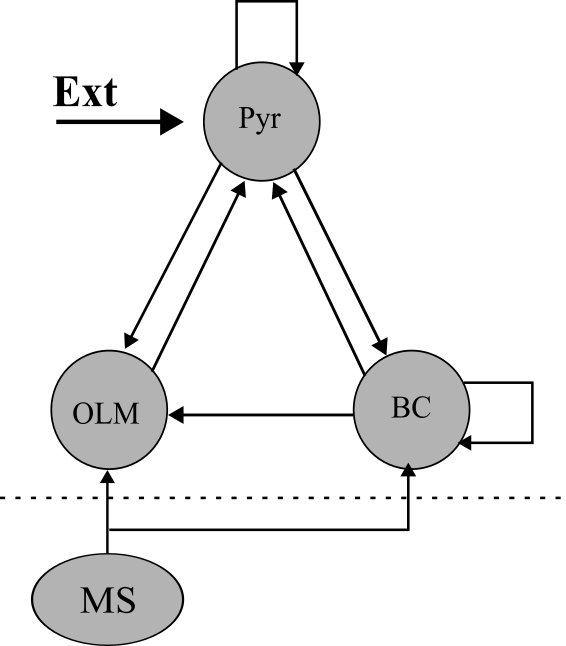
\includegraphics[width=0.7\textwidth]{model_design.png}
    \caption[Schematic of the CA3 network model]{Schematic of the CA3 network model.
        The network comprises of many microcircuits with the connectivity as shown in the above figure. Pyr cells (pyramidal), BC cells (basket cells that inhibit soma),
        O-LM cells (oriens-lacunosum moleculare interneurons that inhibit dendrites), external inputs (mainly from the entorhinal cortex) to Pyr cells, and MS (medial septum).
        BC and O-LM cells are stimulated by Pyr cells, while Pyr cells are inhibited by BC and O-LM cells.
        Recurrent connections among Pyr cells are excitatory, whereas those among BC cells are inhibitory.
        O-LM cells are inhibited by BC cells. The medial septum (MS) delivers inhibitory inputs every 150 ms to BC and O-LM cells.}\label{fig:model_design}
\end{figure}\pagebreak

\section{Model implementation: cell parameters}
The model consists of three types of neurons, each with its own set of
parameters and defined cell classes. The parameters for each cell type are
based on the following references:
\begin{enumerate}
    \item \textbf{Basket Cells}: Modeled after \textcite{wangGammaOscillationSynaptic1996},
          featuring standard dynamics for Na and K currents, along with synaptic and leak currents.
          Each cell is modeled as a single compartment and obeys the following current balance equation:
          \begin{equation}\label{eq:basket_cell}
              C_I \frac{dV_I}{dt} = I_{\text{app},I} - I_{\text{Na},I} - I_{\text{K},I} - I_{\text{L},I} - I_{\text{syn},I}
          \end{equation}

          where \(V_I\) is the membrane potential (mV), \(C_I = 1 \, \mu\text{F/cm}^2\)
          is the membrane capacitance, \(I_{\text{app},I}\) is the applied current, and
          \(I_{\text{syn},I}\) is the total synaptic current. The leak current
          \(I_{\text{L},I} = g_{\text{L},I}(V_I - E_{\text{L},I})\) has a conductance
          \(g_{\text{L},I} = 0.1 \, \text{mS/cm}^2\) and reversal potential
          \(E_{\text{L},I} = -65 \, \text{mV}\). All currents are in units of
          \(\mu\text{A/cm}^2\). The sodium \(I_{\text{Na},I}\) and potassium
          \(I_{\text{K},I}\) currents are voltage-dependent spiking currents of the
          Hodgkin-Huxley type.
    \item \textbf{O-LM Cells}: Adapted from \textcite{saragaActiveDendritesSpike2003},
          including additional currents like hyperpolarization-activated (h) and A-type currents.
          Each cell is modeled as a single compartment and obeys the following current balance equation:
          \begin{equation}\label{eq:olm_cell}
              C_O \frac{dV_O}{dt} = I_{\text{app},O} - I_{\text{Na},O} - I_{\text{K},O} - I_{\text{L},O} - I_{\text{h},O} - I_{\text{A},O} - I_{\text{syn},O}
          \end{equation}

          where \(V_O\) is the membrane potential, \(C_O = 1.3 \, \mu\text{F/cm}^2\) is
          the membrane capacitance, \(I_{\text{app},O}\) is the applied current, and
          \(I_{\text{syn},O}\) is the total synaptic current. The leak current
          \(I_{\text{L},O} = g_{\text{L},O}(V_O - E_{\text{L},O})\) with conductance
          \(g_{\text{L},O} = 0.05 \, \text{mS/cm}^2\) and reversal potential
          \(E_{\text{L},O} = -70 \, \text{mV}\). \(I_{\text{Na},O}\), \(I_{\text{K},O}\),
          \(I_{\text{h},O}\), and \(I_{\text{A},O}\) represent the transient sodium,
          delayed rectifier potassium, hyperpolarization-activated (or h) mixed-cation,
          and A-type potassium currents, respectively, all in units of
          \(\mu\text{A/cm}^2\).
    \item \textbf{Pyramidal Cells}: Based on \textcite{miglioreDendriticIhSelectivelyBlocks2004},
          incorporating compartmentalized dynamics for the complex morphology of pyramidal neurons.
          Each cell is modeled as a multi-compartmental neuron with 5 compartments: 1 for basal dendrites (Bdend),
          1 for soma, and 3 for apical dendrites (Adend1, 2 and 3). Each compartment obeys the following current balance equation:
          \begin{equation}\label{eq:pyramidal_cell}
              C_{E_k} \frac{dV_{E_k}}{dt} = I_{\text{app},E_k} - I_{\text{Na},E_k} - I_{\text{K},E_k} - I_{\text{L},E_k} - I_{\text{h},E_k} - I_{\text{A},E_k} - I_{\text{syn},E_k} + I_{\text{conn},E_k}
          \end{equation}

          where \(V_{E_k}\) is the membrane potential of compartment \(k\), \(C_{E_k}\)
          is the membrane capacitance, \(I_{\text{app},E_k}\) is the applied current,
          \(I_{\text{syn},E_k}\) is the total synaptic current, and
          \(I_{\text{conn},E_k}\) represents the current due to electrical coupling
          between compartments. \(I_{\text{L},E_k}\), \(I_{\text{Na},E_k}\),
          \(I_{\text{K},E_k}\), \(I_{\text{h},E_k}\), and \(I_{\text{A},E_k}\) denote the
          leak, transient sodium, delayed rectifier potassium,
          hyperpolarization-activated mixed-cation, and A-type potassium currents for
          compartment \(k\), respectively.
\end{enumerate}

\noindent For further elaboration of the mathematical formulation of each cell type, see appendix~\ref{ch:appendix_a}.
For the full overview of cell and compartment parameters, see appendix~\ref{ch:appendix_b}.

\section{Model implementation: synaptic connections}
The model contained three types of synaptic connections: excitatory, inhibitory
based on AMPA, NMDA and GABA-A receptors. Synapses were modeled by standard
NEURON double-exponential mechanism. This approach entailed the assignment of
specific rise \(\tau_1\) and decay \(\tau_2\) time constants, which correspond
to the temporal profiles of conductance increase and subsequent decline,
respectively, following a synaptic event. The conductance values, indicative of
synaptic efficacy, were varied according to the type of presynaptic and
postsynaptic neuron pairing, as well as the subtype of receptor involved (AMPA,
NMDA, or GABA-A). These parameters informed the simulation of synaptic inputs,
which govern the depolarization and hyperpolarization events in the
postsynaptic neuron membrane, thereby influencing the temporal patterns of
neuronal firing and network activity. These parameters adhere to the following formula:

\begin{equation}\label{eq:synaptic_conductance}
    g(t) = \frac{g_{\text{max}}}{\tau_2 - \tau_1} \left( e^{-\frac{t}{\tau_2}} - e^{-\frac{t}{\tau_1}} \right)
\end{equation}

The synaptic conductance at a given time \(t\) after a presynaptic spike is represented by \(g(t)\), where \(g_{\text{max}}\) indicates the peak conductance measured in NanoSiemens (nS).
The rise and decay of the synaptic conductance are characterized by the time constants \(\tau_1\) and \(\tau_2\), respectively, both of which are measured in milliseconds (ms).
Here, \(t\) stands for the time elapsed following the arrival of the presynaptic spike.
This model effectively describes the dynamic behavior of synaptic conductance, which initially rises during the onset phase and subsequently undergoes a more prolonged decrease, a pattern common to both excitatory and inhibitory postsynaptic potentials (EPSPs and IPSPs).
The variation in the time constants \(\tau_1\) and \(\tau_2\) facilitates the adjustment of the synaptic response's time profile, with \(\tau_1\) influencing the speed of onset and \(\tau_2\) affecting the length of the conductance alteration.
For the parameters used, see Table~\ref{table:compartment_dependent_parameters} and~\ref{tab:synaptic_parameters}.
\begin{table}[htbp]
    \centering
    \caption[Compartment dependent parameters]{Compartment dependent parameters used in the formulations of the three neuronal cell types according to equation~\ref{eq:synaptic_conductance}.
        See appendix~\ref{ch:appendix_a} for the full equations.
        The ionic conductances are in mS/cm\(^2\).}\label{table:compartment_dependent_parameters}
    \begin{tabular}{l|cccccccccc}
        \hline
        \hline
               & \( g_{h} \) & \( g_{A} \) & \( g_{Na} \) & \( g_{K} \) & \( V_{50} \) & \( b \) & \( c \) & \( d \) & \( e \) & \( f \) \\
        \hline
        Bdend  & 0.1         & 48          & 32           & 10          & -82          & 1       & 4       & 1.5     & 11      & 0.825   \\
        Soma   & 0.1         & 48          & 32           & 10          & -82          & 0.8     & 4       & 1.5     & 11      & 0.825   \\
        Adend1 & 0.2         & 72          & 32           & 10          & -82          & 0.5     & 4       & 1.5     & 11      & 0.825   \\
        Adend2 & 0.4         & 120         & 32           & 10          & -90          & 0.5     & 2       & 1.8     & -1      & 0.7     \\
        Adend3 & 0.7         & 200         & 32           & 10          & -90          & 0.5     & 2       & 1.8     & -1      & 0.7     \\
        \hline
        \hline
    \end{tabular}
\end{table}
\pagebreak

\noindent
The synaptic connections between neurons were implemented
as follows:

\begin{table}[htbp]
    \centering
    \caption[Synaptic Parameters for the Connectivity Between Neurons in the Model]{Synaptic Parameters for the Connectivity Between Neurons in the Model: Pre- and postsynaptic receptor types are given for each cell type.
        The time constants \(\tau_1\) and \(\tau_2\) are in milliseconds.
        \(\tau_1\) is the rise time constant, the time it takes for synaptic conductance to increase from baseline to peak.
        \(\tau_2\) is the decay time constant, the time it takes for the conductance to decrease from peak to baseline.
        The conductance indicates the strength of the synaptic connection and its ability to conduct ionic current across the postsynaptic membrane.
        This influences the extent to which the synaptic input can depolarize the postsynaptic neuron and is in nanoSiemens (nS).}\label{tab:synaptic_parameters}
    \begin{tabular}{lllccc}
        \hline
        Presynaptic & Postsynaptic & Receptor & \(\tau_1\) (ms) & \(\tau_2\) (ms) & Conductance (nS) \\
        \hline
        Pyramidal   & Pyramidal    & AMPA     & 0.05            & 5.3             & 0.02             \\
        Pyramidal   & Pyramidal    & NMDA     & 15              & 150             & 0.004            \\
        Pyramidal   & Basket       & AMPA     & 0.05            & 5.3             & 0.36             \\
        Pyramidal   & Basket       & NMDA     & 15              & 150             & 1.38             \\
        Pyramidal   & OLM          & AMPA     & 0.05            & 5.3             & 0.36             \\
        Pyramidal   & OLM          & NMDA     & 15              & 150             & 0.72             \\
        Basket      & Pyramidal    & GABA-A   & 0.07            & 9.1             & 0.72             \\
        Basket      & Basket       & GABA-A   & 0.07            & 9.1             & 4.5              \\
        Basket      & OLM          & GABA-A   & 0.07            & 9.1             & 0.0288           \\
        OLM         & Pyramidal    & GABA-A   & 0.2             & 20              & 72               \\
        MS          & Basket       & GABA-A   & 20              & 40              & 1.6              \\
        MS          & OLM          & GABA-A   & 20              & 40              & 1.6              \\
        \hline
    \end{tabular}
\end{table}

\noindent For the full overview of synaptic parameters, see appendix~\ref{ch:appendix_b}.
\pagebreak

\section{Model implementation: stimulation and noise}
The model was activated by external inputs originating from the entorhinal
cortex, which were then transmitted to the pyramidal cells. Background random
excitatory and inhibitory inputs were received by the O-LM, basket cells, and
the soma of the pyramidal cells via their AMPA, NMDA, and GABA-A receptors as
shown in Table~\ref{tab:synaptic_parameters}. The mechanism by which noise was
applied to the model was defined via NEURON simulator's \textit{NetStim}
object. This object type generated spike train according to a set of parameters
such as stimulus interval, noise variability (Poisson-like), weight, target,
start and delay times. These parameters can be viewed in Appendix A.

Similarly, the distal dendritic compartments of the pyramidal cells also
received comparable inputs through the same types of receptors. Connections
such as O-LM to pyramidal cell, basket to pyramidal cell, basket-basket
recurrent connections, and medial septum to O-LM and basket cell connections
were mediated through GABA-A receptors. Additionally, the medial septum
provided inhibitory inputs to the basket and O-LM cells at intervals of 150 ms.

\section{Simulations}
For the simulations, the model was implemented in NEURON version 7.6.3. The
simulations were run on a Linux GNOME (v22.04) desktop computer with 2 Xeon CPU
E5--2699 v3 CPUs with 32 physical cores @ 2.3GHz for multi-threading, a Nvidia
GTX 4060 graphics card, and 256 GB of RAM\@. Trials were run for 5000 ms with a
time integration step of 0.1 ms resulting in 50.000 simulation steps per trial
dataset. Random seeds were used to generate the external noise, connections and
cells for each trial and remained constant between trials and between
experiments. The number of trials varies between experiments and are specified
in their respective sub-sections that follow. In the network, the individual
cells were assigned a global identifier (GID) to which all the data was
associated in the same ascending order for each trial. The first 800 cells were
always pyramidal cells, the next 200 were basket cells and the last 200 were
O-LM cells. For each trial, the individual cell spike times were saved for the
entire duration of the simulation. Pyramidal cell membrane soma voltage data
was saved per cell in order to calculate the LFP signal (necessary for
theta-gamma calculations). In all simulations the LFP is calculated by
taking the sum of the differences in membrane potential of the distal apical
and basal dendritic compartments of all cells in the pyramidal population.

\subsection{Baseline activity}
In order to obtain baseline activity in the network as shown in Figure
~\ref{fig:model_design}, current injections were added (\textbf{Pyramidal
    cells:} 50 pA\@; \textbf{O-LM cells:} -25 pA). At Baseline, the network
generates theta-modulated gamma oscillations activity. This activity was
measured from the Local Field potential (LFP) in the network. The LFP was
simulated by a sum difference between membrane potential of the distal apical
and basal dendritic compartment over all pyramidal cells. As discussed in the
cell parameters section, all cells contained leak current, transient sodium
current \(I_{\text{Na}}\), and delayed rectifier current \(I_{K, \text{-}
        \text{dr}}\) to allow for action potential generation. On average, the firing
rates were \(2.36 \pm 0.024\) Hz for pyramidal cells, \(16.05 \pm 0.15\) Hz for
basket cells and \(0.96 \pm 0.027\) Hz for O-LM interneurons at baseline in the
original \parencite{sanjayImpairedDendriticInhibition2015}. However, it should
be noted that our custom implementation of the same model had a slightly
lowered baseline (see the results section). The reason for this discrepancy is
unknown and is a potential source of error in the results. 50 trials total were
done for the baseline activity and averaged.

\subsection{Model validation}
In order to test the implementation of the model, results from the article were
replicated, namely Figures 6A, B and C from
\textcite{sanjayImpairedDendriticInhibition2015}. In this replicated experiment
the O-LM to pyramidal cells connection weight was reduced in decrements of 0.1x
times the baseline from 1.0 to 0.0. In addition to reduced connection strength,
the external noise fed into the pyramidal cells was increased in increments of
0.1X times the baseline from 1.0 to 2.0. By reducing the connectivity from O-LM
to pyramidal cells, dendritic inhibition was impaired and potential
epileptiform activity was induced.

The original results on which the validation experiment focussed on, were the
following three aspects: changes in firing rates per population, the changes in
dominant theta and gamma frequencies, and finally the changes in the power of
the theta and gamma oscillations (see
Figure:~\ref{fig:validation_original_results}). The numerical results from are
in the following table:

\begin{table}[htbp]
    \centering
    \caption[Summary of Original Network Simulation Parameters and Results]{Overview of Original Network Simulation Settings and Outcomes.
        This table contains all the original results of Figure 6 from the \textcite{sanjayImpairedDendriticInhibition2015} article.
        Variations in the firing rates of single cells, alongside theta and gamma oscillations within the local field potential, as well as the alterations in their intensity upon the decrease of dendritic inhibition and the concurrent enhancement of external stimuli to the pyramidal neurons.}\label{tab:original_validation_results}
    \begin{adjustbox}{width=\textwidth}
        \begin{tabular}{ccccccccc}
            \hline
            OLM-Pyr Wt & External Wt & \CellWithForcedBreak{Pyr (Hz)                                                          \\ + Std} & \CellWithForcedBreak{BWB (Hz) \\ + Std} & \CellWithForcedBreak{OLM (Hz) \\ + Std} & \CellWithForcedBreak{Theta \\ Freq (Hz)} & \CellWithForcedBreak{Theta power \\ (mV\textsuperscript{2} Hz\textsuperscript{-1})} & \CellWithForcedBreak{Gamma \\ Freq (Hz)} & \CellWithForcedBreak{Gamma power \\ (mV\textsuperscript{2} Hz\textsuperscript{-1})} \\
            \hline
            1x         & 1x          & 2.36 ± 0.024                  & 16.05 ± 0.15 & 0.96 ± 0.027 & 6.7 & 5.35 & 33.2 & 2.55 \\
            0.8x       & 1.2x        & 2.66 ± 0.029                  & 19.88 ± 0.11 & 1.11 ± 0.03  & 6.7 & 5.4  & 32.5 & 2.4  \\
            0.6x       & 1.4x        & 2.9 ± 0.03                    & 21.04 ± 0.15 & 1.42 ± 0.03  & 6.7 & 4.1  & 32.4 & 5.3  \\
            0.4x       & 1.6x        & 3.19 ± 0.033                  & 22.15 ± 0.15 & 1.93 ± 0.03  & 6.7 & 2.2  & 31.7 & 3.6  \\
            0.2x       & 1.8x        & 3.67 ± 0.036                  & 23.97 ± 0.15 & 2.64 ± 0.036 & 6.7 & 2    & 32.7 & 6.5  \\
            0.1x       & 1.9x        & 4.24 ± 0.038                  & 26.98 ± 0.15 & 3.35 ± 0.034 & 6.7 & 1.16 & 33.9 & 11.4 \\
            0.05x      & 1.95x       & 4.5 ± 0.04                    & 21.68 ± 0.25 & 3.69 ± 0.033 & 6.7 & 0.65 & 37.8 & 1.55 \\
            0x         & 2x          & 6.14 ± 0.054                  & 24.26 ± 0.44 & 4.98 ± 0.035 & 0   & 0    & 38.8 & 1.32 \\
            \hline
        \end{tabular}
    \end{adjustbox}
\end{table}

\begin{figure}[htbp]
    \centering
    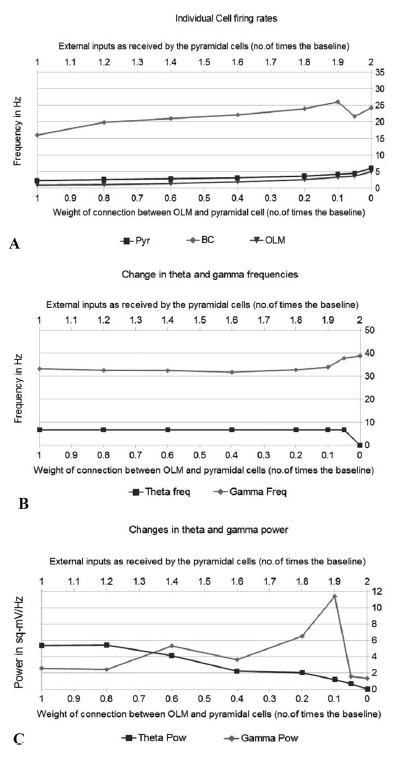
\includegraphics[width=0.65\textwidth]{model_validation_original_results.png}
    \caption[\textcite{sanjayImpairedDendriticInhibition2015} article results]{\textcite{sanjayImpairedDendriticInhibition2015} article results: Figure 6.
        A validation experiment was conducted to replicate the results of scenario 2 from the original article.
        This was done in order to verify the implementation of the model. The experiment involved reducing the
        connection strength from O-LM to pyramidal cells and increasing the
        external noise fed into the pyramidal cells. The firing rates per population (A), dominant frequencies in the theta-gamma bands (B) and their respective average power (C) was investigated.
        The results were compared to the original article to verify the implementation of the model (see Results section).}\label{fig:validation_original_results}
\end{figure}

\subsection{Sodium and potassium variants}
In this experiment, the sodium and potassium conductances of the all cell types
cells were changed from 0.5x to 1.5x times the baseline in increments of 0.1.
The changes were induced in separate experiments for each of the three cell
types, so 6 experiments in total were conducted: 3 for sodium and 3 for
potassium. These induced changes were done in order to investigate the effect
of the conductances on the network activity and the influence of individual
cell types on the same metrics as in the model validation experiment. 20 trials
each were done per condition (6 total conditions) and the results were
averaged.

\subsubsection{Visualization of Neuronal Activity Variants}
This section outlines the analytical approach adopted for visualizing the
neuronal activity within our network model under different experimental
conditions. Specifically, we focused on plotting the firing rates, theta-gamma
frequencies, and theta-gamma power across all neuronal populations (pyramidal,
basket, and O-LM cells) for variants induced by alterations in sodium and
potassium conductance levels.

\subsubsection{Firing Rate Analysis}
We initiated our analysis by examining the firing rates across different cell
populations. A comparative visualization was generated to juxtapose the mean
firing rates under sodium and potassium variant conditions, utilizing a grid
layout for a side-by-side comparison. Each plot incorporated error bars to
represent the standard error of the mean (SEM), thereby conveying the
variability inherent in our simulation trials. Cell populations were
differentiated by distinct markers and colors to facilitate clear distinction
between pyramidal, basket, and O-LM cells across varying conditions.

\subsubsection{Theta-Gamma Frequency Analysis}
Subsequent to firing rate analysis, we delved into the investigation of theta
and gamma frequency bands. For each variant type (sodium and potassium), theta
and gamma frequencies were plotted on a \(2\times2\) grid, delineating the mean
frequency values extracted from the simulation data. This approach allowed for
an intuitive understanding of the oscillatory dynamics prevalent in the network
under different ionic conductance conditions, highlighting potential shifts in
theta-gamma coupling associated with epileptiform activities.

\subsubsection{Theta-Gamma Power Analysis}
In addition to the frequency analysis, the power of theta and gamma oscillations were quantified.
This step aimed to investigate the intensity of oscillatory activity within these critical frequency bands.
Similar to our frequency analysis, a \(2\times2\) grid layout facilitated the comparison of theta and gamma power
across sodium and potassium variants. This visual representation served to
elucidate variations in oscillatory power, potentially correlating with changes
in network excitability and synchronization under altered ionic conditions.

\subsubsection{Power Spectral Density (PSD) Calculation}
The aforementioned theta-gamma analyses used the \lstinline{calc_psd} function to compute the power spectral density (PSD) of an LFP signal, focusing on theta (3--12 Hz) and gamma (30--80 Hz) frequencies.
Initial signal processing includes discarding the first millisecond to avoid transient effects and down-sampling according to a predefined maximum frequency (\textit{fmax}).
The PSD calculation uses a Fast Fourier Transform (FFT) approach, adjusting for the signal mean.
For both theta and gamma ranges, the function identifies relevant frequencies, calculates mean power by averaging power values within these ranges, and identifies the dominant frequency by locating the frequency with the maximum power value.
This analysis facilitated the quantification of signal power and rhythmic activity within specific frequency bands, essential for understanding neural dynamics in these ranges.

\subsection{External noise variants}
In this experiment, the external noise fed into the distal dendrites of
pyramidal cells was set a new baseline for the 1.0x condition, which was 20 times that of the original
\textcite{sanjayImpairedDendriticInhibition2015} model. Excitatory inputs were fed through
AMPA and NMDA receptors. Reduced O-LM to pyr connections were kept at 10\% of
the original baseline. This was done because in the original article, epileptic activity was induced by feeding in 20 times
more external noise at reduced dendritic inhibition.

This condition was tested as a special condition in Figure 7 of the article,
and was expanded upon because of the occurrence of a depolarization block in
the basket cell spike activity. This depolarization block occurrence was
assumed to be the epileptic state in which the network is found at such
conditions. This new baseline was changed times a range of pyramidal noise
factors of the following values: 0.65, 0.70, 0.75, 0.80, 0.85, 0.90, 0.95,
1.00, 1.10, 1.20, and 1.30. In addition to the range of noise factors,
pyramidal conductances \(g_{\text{Na}}\) and \(g_{\text{K}}\) were modified
over a range of 0.5x to 1.5x times the baseline in increments of 0.1. 15 trials
were done per noise condition and the results were averaged.

\subsubsection{Detection of epileptiform activity (Experiments: External Noise and Recurrent Connection strength variants)}
The detection of epileptic activity depends on the spiking activity of the
basket cells, which according to results of Figure 7 from the
\textcite{sanjayImpairedDendriticInhibition2015} article occurs in the presence
of great external drive from the pyramidal cells of at least 20 times the
baseline and with reduced dendritic inhibition by the O-LM cells. Detection of a
depolarization block in the basket cells was done by calculating the convoluted
fire rates of the basket cell population.


\noindent The systematic approach to analyzing basket cell firing rates through convolution with a Gaussian window was as follows:
\begin{itemize}
    \item \textbf{Extracting Spike Times:} The \lstinline{get_spike_times_for_basket_cells}
          function is used for iterating over a range of GIDs. This process collects spike times from
          all basket cells and concatenates them, constructing a continuous signal of neural activity.

    \item \textbf{Creating Time Series:} Spike times are converted into a binary series
          using \lstinline{create_time_series}. Each neural firing event is denoted by a '1' in a
          zero-initialized array at the corresponding time index.

    \item \textbf{Applying Gaussian Convolution:} The \lstinline{apply_gaussian_convolution}\newline
          function smooths the time series. It convolves the series with a Gaussian window, normalized
          to sum to one, yielding a signal that mirrors the firing rates over time.

    \item \textbf{Summing Convolved Signals:} Collective firing behavior is analyzed by
          \lstinline{get_convolved_signal_per_neuron}. It applies Gaussian convolution to individual
          neuron time series and sums them, forming an aggregated firing rate signal.

    \item \textbf{Detecting Depolarization Blocks:} The \lstinline{detect_depolarization_blocks}
          function identifies reduced activity periods by analyzing the convolved signal for intervals
          that remain below a set threshold for a specified minimum duration.
\end{itemize}

\noindent
This method for detecting depolarization blocks in the basket cell population
and convolution of spike activities was also used for the recurrent
connection strength variants experiment below. See the example in Figure~\ref{fig:depolarization_block_basket_cells}.

\begin{figure}[htbp]
    \centering
    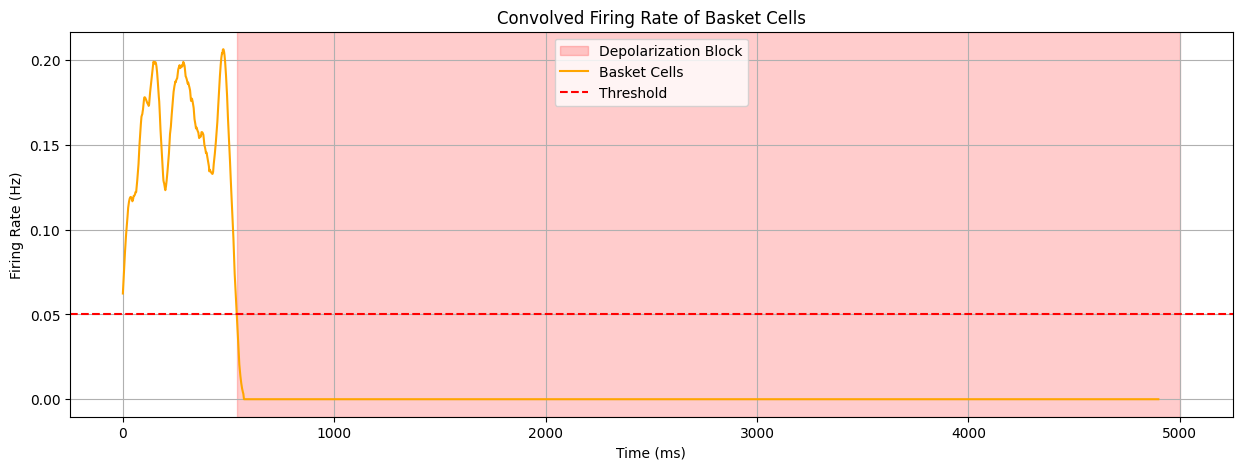
\includegraphics[width=1.0\textwidth]{Depolarization_block_basket_cells.png}
    \caption[Depolarization block in basket cells]{Depolarization block in basket cells. Example of a single trial where a depolarization block is found in the convoluted spike activity signal as a flat-line at 0 Hz. The firing rate is in Hz (y-axis) and the signal is calculated over the entire duration of the trial (5000 ms).
        Note that the signal has to pass the threshold for an extended period of 100 ms to be considered a DPB\@.
        In addition, the first 50 ms are excluded from detection to avoid false positives. This detection method was done for each individual trial.}\label{fig:depolarization_block_basket_cells}
\end{figure}
\pagebreak

\subsubsection{Analysis of External Noise Variants}
This section elaborates on the methodological approach undertaken to assess the
impact of varying levels of external noise on pyramidal cells, with the aim of
understanding its influence on depolarization block occurrences within the
network. The experiment's premise was based on the hypothesis that adjusting
the external noise could modulate the epileptic state, characterized by
depolarization blocks, within the neural network.\\

\noindent The analysis was structured as follows:
\begin{enumerate}
    \item \textbf{Event Detection and Quantification:} For each variant of external noise levels, depolarization events were systematically identified. These results were quantified per trial. This process involved the enumeration of depolarization events, accumulation of their start and end times, and the computation of the overall duration of these events within each trial.

    \item \textbf{Statistical Analysis:} Subsequent to the detection of depolarization events, the analysis proceeded with the calculation of average event duration and the computation of the percentage of trials exhibiting depolarization blocks. Furthermore, the mean delay and standard deviation for the onset of depolarization events were determined to gauge the temporal dynamics of the network's response to varying noise levels.

    \item \textbf{Data Visualization:} To concisely present the findings, the analysis results were visualized through matrix plots. These plots delineated the relationship between pyramidal conductances (\(g_{\text{Na}}\) and \(g_{\text{K}}\)) and the observed network behavior under different external noise conditions. The visualizations highlighted the proportion of trials with depolarization blocks and detailed the temporal onset characteristics of these events, facilitating an intuitive understanding of the network's epileptic susceptibility.
\end{enumerate}

\noindent The investigative focus on external noise variants sought to delineate
the conditions under which the network transitions into an epileptic state, as indicated by the
presence of depolarization blocks and the average delay in the onset of a DPB (including STD).
\pagebreak
\subsection{External noise: Burst analysis}
Further analysis was conducted to investigate the burst dynamics of pyramidal
and basket cell activity based on the observations done in the initial
increased noise experiment. This experiment involved looking at the temporal
shift in detected bursts surrounding the onset of a depolarization block event
in the basket cell population.

\subsubsection{Detection of Epileptiform Activity and Burst Analysis}
This experiment employed leveraging convolved spike activities and burst detection within
neural populations to detect epileptiform activity. The approach was predicated on analyzing the temporal
dynamics of neuronal firing rates, specifically focusing on the basket and
pyramidal cell populations. A critical aspect of this analysis was the
identification and analysis of bursts in relation to the onset of
depolarization blocks (DPBs), including the possible variance in burst intensity.\\

\noindent The unified methodology proceeded as follows:
\begin{itemize}
    \item \textbf{Identification of Depolarization Block Onset:} A custom python function \lstinline{find_depolarization_block} was employed to scan the simulation data for periods devoid of spiking activity within a specified window across basket cell populations.
          This step was crucial in pinpointing the initial point of a depolarization block, thus serving as a reference for the subsequent analysis.

    \item \textbf{Preparation and Convolution of Spike Activities:} Spike times were aggregated and subjected to a Gaussian filter, smoothing the data to represent neural firing rates over time effectively.
          This step facilitated the identification of significant patterns in relation to the DPB onset.

    \item \textbf{Burst Detection and Temporal Analysis:} The convolved spike activities were analyzed using a burst detection algorithm, identifying significant increases in activity as bursts.
          These were classified based on their occurrence relative to the DPB onset—focusing on the last burst before, the second-last burst before, and the first burst after the onset. This classification shed light on the changes in neural dynamics preceding and following a depolarization block.

    \item \textbf{Analytical Assessment and Summarization of Findings:} Start and end times were determined for detected bursts, as well as peak activity levels.
          This comprehensive analysis of convolved spike activities and burst dynamics provided a detailed view of the neural mechanisms during critical phases of epileptiform activity.
\end{itemize}

\noindent The experiment utilized a 100 ms window and a 0.1 ms time step throughout the 5000 ms simulation duration, resulting in 50,000 indices for spike detection.
The absence of basket cell firing within this window indicated a DPB, which was critical for burst detection.
This methodology offered a nuanced understanding of epileptiform dynamics, highlighting the transitions of neural populations into and out of depolarization blocks which are indicative of epileptic activity in the network.
Note that in the burst analysis the 1D-Gaussian convolution was performed on a histogram of the spike times of cells. Whereas in the previous convolution for the matrices, the convolutions were performed using a binary time series of the spike times.

\begin{figure}[htbp]
    \centering
    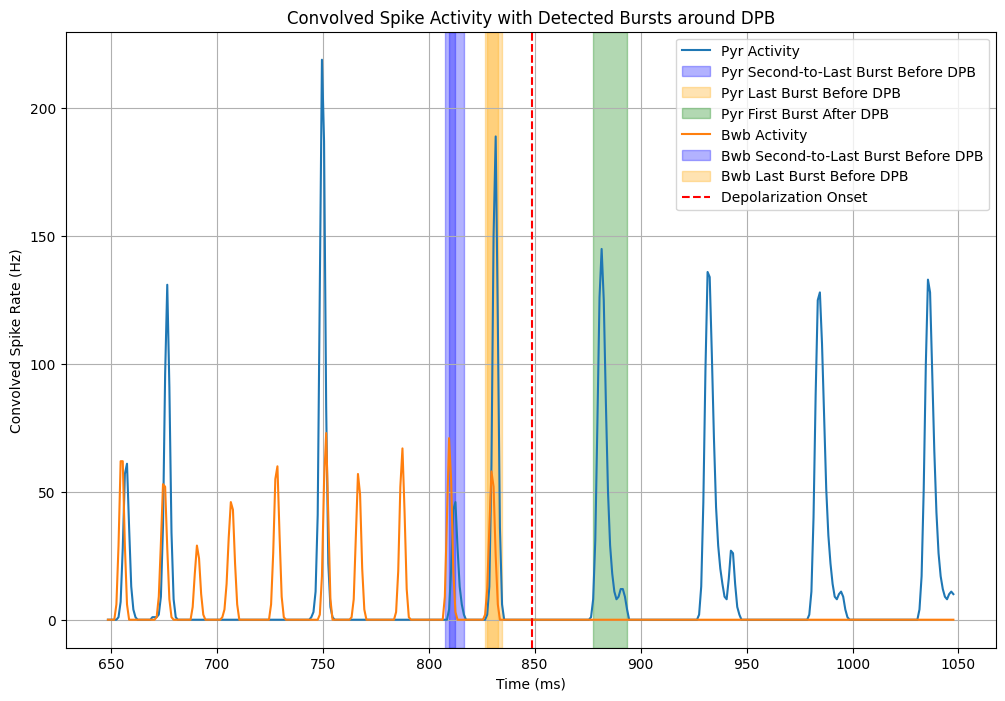
\includegraphics[width=1.0\textwidth]{Convolved_Burst_detection_DPB_example.png}
    \caption[Burst detection example]{Burst detection example. Example of a single trial where bursts in the neural populations are detected near the onset of a DPB using convoluted spike activity signals. The firing rate is in Hz (y-axis) and the signal is calculated over the entire duration of the trial (5000 ms).
        The onset of a depolarization block in basket cells is indicated by a red dashed vertical line. The last and second to last bursts before, and the first burst after the DPB were detected and used for analysis.
        Note that the signal has to pass the threshold for an extended period of 100 ms to be considered a DPB\@.
        In addition, the first 50 ms are excluded from detection to avoid false positives. This detection method was done for each individual trial.}\label{fig:example_burst_detection}
\end{figure}
\pagebreak

\subsection{Recurrent connection strength variants}
This section describes the methodology employed to analyze the effects of
varying recurrent connection strengths between basket cells on the incidence
and characteristics of depolarization blocks within the network. This analysis
aimed to explore the potential of modulating soma inhibition strength to
mitigate epileptic activity and restore baseline network dynamics.

The experiment adjusted the recurrent connection strength across a range of
multipliers (1.00, 1.05, 1.10, 1.15, and 1.20 times the baseline), concurrently
with modifications to \(g_{\text{Na}}\) and \(g_{\text{K}}\) within a plus or
minus 25\% range of the baseline. The connection weight from O-LM cells to
pyramidal cells was fixed at 10\%, facilitating the induction of depolarization
blocks under a 20x external noise condition on pyramidal cells. A total of 15
trials were conducted for each condition, and the results were averaged for
analysis.

\subsubsection{Analysis of Recurrent Connection Strength Variants}
\noindent The analysis procedure was as follows:
\begin{enumerate}
    \item \textbf{Event Detection and Aggregation:} The analysis began by identifying depolarization events across trials for each variant of the recurrent connection strength. This involved counting the number of depolarization events, their start and end times, and the total duration of depolarization within each trial. Trials devoid of depolarization events were separately tallied.

    \item \textbf{Statistical Computation:} For trials exhibiting depolarization events, the average duration of these events was calculated. Additionally, the percentage of trials manifesting depolarization events and the statistical measures (mean and standard deviation) concerning the onset times of these events were determined.

    \item \textbf{Matrix Visualization:} The analyzed data were visualized using matrix plots to illustrate the relationship between the recurrent connection strength variants and the properties of depolarization events under different \(g_{\text{Na}}\) and \(g_{\text{K}}\) conditions. These plots highlighted the percentage of trials with depolarization blocks and the count of depolarization events, offering insights into the efficacy of soma inhibition strength adjustments in modulating epileptic activity.
\end{enumerate}

\noindent
This analytical approach facilitated a comprehensive examination of the impact of modifying recurrent connection strengths among basket cells on the network's susceptibility to epileptic disruptions.
Through statistical and visual analyses, the dynamics governing epileptiform activity and the potential for intervention was investigated through targeted manipulation of inhibition mechanisms within the neural circuitry.
\pagebreak

\noindent For detecting depolarization blocks in the basket cell population, the
methodology was as follows:
\begin{itemize}
    \item Establishing a signal threshold indicating a depolarization block.
    \item Excluding initial transient analysis to prevent false positives.
    \item Identifying threshold crossings that mark the start and end of depolarization
          blocks.
    \item Applying a minimum duration filter to these blocks.
    \item Summarizing and reporting the total duration of all valid depolarization blocks
          in the trial.
\end{itemize}

\noindent A check was performed if the convoluted signal remained beneath a fixed
threshold of 0.001 for at least 100 ms. This threshold was defined non-zero,
yet tiny as in the depolarization block there are no firing neurons in the
basket population. The first 50 ms of the signal were excluded to avoid false
positives. If the signal remained beneath the threshold for at least 100 ms,
the condition was considered to be in a depolarization block state. This was
done for each trial individually. An example of this can be seen in Figure~\ref{fig:depolarization_block_basket_cells}.


\chapter{Results}

\todo[inline]{fix the captions for the figures, see the article for the correct captions.}

\section{Results of the Baseline activity}
In the initial experiment, the baseline activity of the CA3 network was
observed from the \textit{original model} by
\textcite{sanjayImpairedDendriticInhibition2015}. The network was simulated for
5000 ms and showed synchronous activity throughout all three
populations (pyr, BC and OLM). Basket cells showed a higher firing rate
compared to the pyramidal cells and O-LM cells. The basket cells also swapped
between states of synchrony and asynchrony which was not observed in the other
two populations. The O-LM cells showed the lowest firing rate compared to the
pyramidal cells and basket cells. The baseline activity of the CA3 network is
shown in figure~\ref{fig:baseline_activity}.

The average firing rates of the populations were 2.36 ± 0.024 Hz for pyramidal cells, 
16.05 ± 0.15 Hz for basket cells, and 0.96 ± 0.027 Hz for O-LM interneurons, 
similar to observed results from \textcite{neymotinKetamineDisruptsTheta2011} which used the same model on which the Sanjay model is based upon.

Just as reported in the original article, the network produces theta-modulated gamma oscillations 
within the local field potential (LFP). These oscillations were influenced by signals from the Medial Septum (MS). 
The gamma oscillations emerged from the inhibitory connections between basket cells that inhibit somas of pyramidal and O-LM cells, 
as well as interactions among basket cells themselves. Conversely, theta oscillations were the result of interactions between 
pyramidal cells and O-LM cells that inhibit dendrites. The network achieved a consistent theta frequency of 6.7 Hz due to periodic inputs 
from the MS to both O-LM and basket cells every 150 ms. The frequency of the gamma component within the LFP was approximately 33 Hz. 
Despite receiving similar MS inputs as O-LM cells, the impact on basket cells was significantly reduced because of their mutual interactions 
and the enhanced influence from pyramidal cells.

\begin{figure}[htbp]
    \centering
    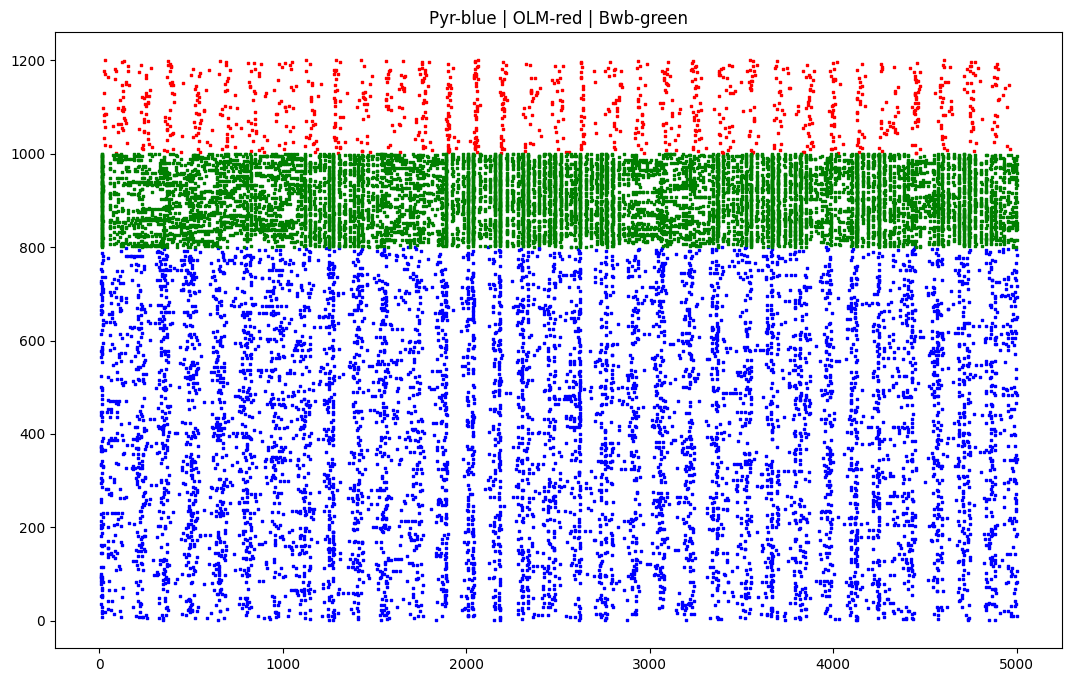
\includegraphics[width=1.0\textwidth]{Network_spike_activity_OLM_baseline.png}
    \caption[Baseline activity of the CA3 network]{Baseline activity of the CA3 network.}\label{fig:baseline_activity}
    \begin{minipage}{0.9\textwidth}
        The above figure shows the baseline activity of the CA3 network. The network was simulated for 5000 ms. 
        The spike activity in time of the Pyr cells, BC cells, and OLM cells are shown based on the Neuron ID\@. 
        ID 0--799 = Pyramidal (blue), 800--999 = BC (green), 1000--1200 = OLM (red). 
        The x-axis represents the time in ms and the y-axis represents the neuron ID\@.
    \end{minipage}
\end{figure}
\pagebreak
\section{Results of the Model validation}
To test whether our implementation of the CA3 network was able to replicate
more elaborate results, results from figure 6 of the original
\textcite{sanjayImpairedDendriticInhibition2015} article were replicated in
figure~\ref{fig:validation_firing_rates},~\ref{fig:validation_frequencies} and
~\ref{fig:validation_power}.

Like in the original experiment, O-LM-pyramidal connectivity was decreased in decrements of 0.1 and reduced dendritic inhibition.
Simultaneously, external noise fed to pyramidal cells via AMPA and NMDA at the synaptic level was increased in increments of 0.1. 
When O-LM-pyramidal connectivity was decreased to a range of 20--10 \%, desynchronization was observed among basket cells (figure~\ref{fig:scatterplot_20_con_olm_pyr}).
Complete desynchronization was observed when the O-LM-pyramidal connectivity was reduced to 0 \% (figure~\ref{fig:scatterplot_0_con_olm_pyr}).
Pyramidal to O-LM connectivity was was unchanged, thus these cells showed sustained synchronous activity.

\begin{figure}[htbp]
    \centering
    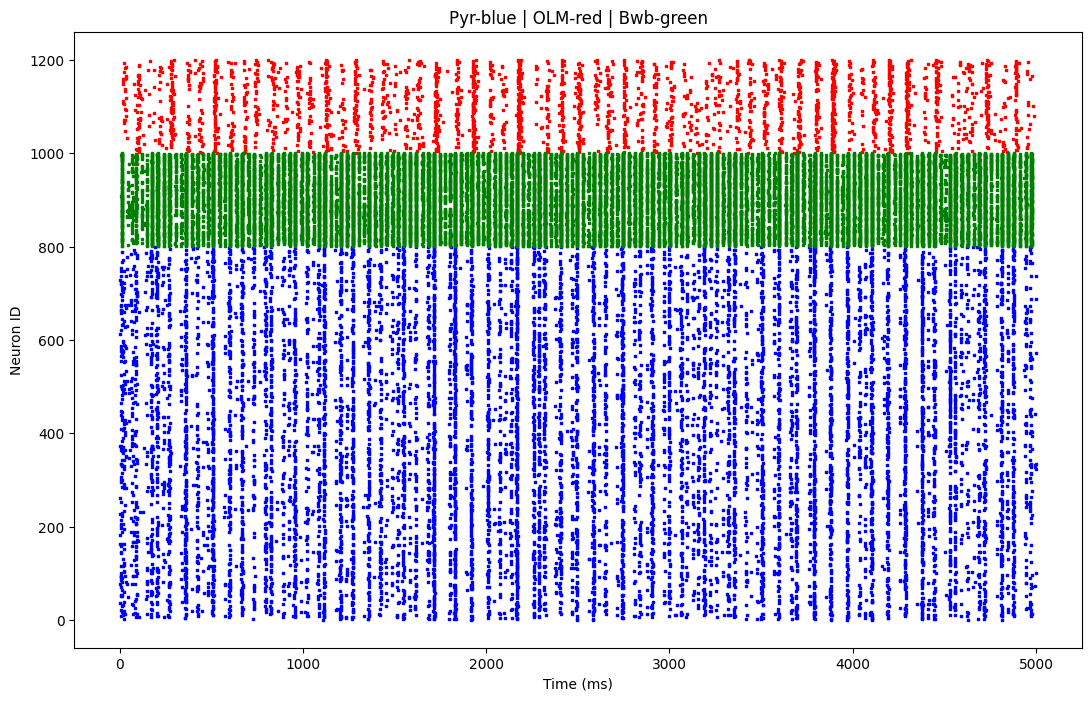
\includegraphics[width=1.0\textwidth]{Olm_pyr_20_con_scatter.png}
    \caption[20 \% OLM-Pyr connection scatter plot]{Scatter plot of the network activity at 20 \% OLM-Pyr connection}\label{fig:scatterplot_20_con_olm_pyr}
    \begin{minipage}{0.9\textwidth}
        The above figure shows the network activity at 20 \% OLM-Pyr connection with significant asynchrony amongst the basket cells.
        The network was simulated for 5000 ms. 
        The scatter plot shows the spike activity of the Pyr cells (blue), BC cells (green), and OLM cells (red). 
        The x-axis represents the time in ms and the y-axis represents the neuron ID\@. 
    \end{minipage}
\end{figure}

\begin{figure}[htbp]
    \centering
    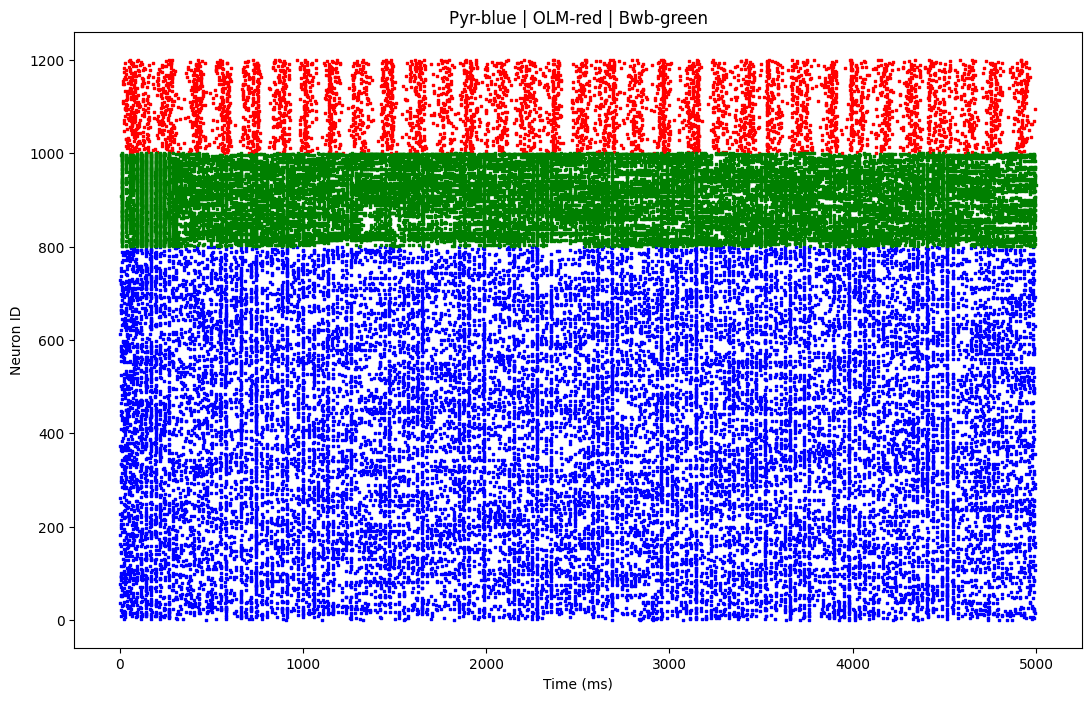
\includegraphics[width=1.0\textwidth]{Olm_pyr_no_connection_scatter.png}
    \caption[0 \% OLM-Pyr connection scatter plot]{Scatter plot of the network activity at 0 \% OLM-Pyr connection}\label{fig:scatterplot_0_con_olm_pyr}
    \begin{minipage}{0.9\textwidth}
        The above figure shows the network activity at 0 \% OLM-Pyr connection with complete asynchrony amongst the basket cells.
        The network was simulated for 5000 ms. 
        The scatter plot shows the spike activity of the Pyr cells (blue), BC cells (green), and OLM cells (red). 
        The x-axis represents the time in ms and the y-axis represents the neuron ID\@. 
    \end{minipage}
\end{figure}

The results show that the model was able to
replicate the results of the original article with slightly lower firing rates,
theta-gamma frequencies and power, which can be seen in
table~\ref{tab:validation_results}. The original article results are visible in
the methods section in table~\ref{tab:original_validation_results} for comparison.

For the firing rates in figure~\ref{fig:validation_firing_rates},
there was a notable increase in the firing rates of all neuron types as dendritic inhibition was 
decreased while external noise was simultaneously increased.
The individual cell firing frequencies showed a near linear increase throughout in both pyramidal and O-LM cells, 
being most pronounced in the basket cell population.
The basket cell population also showed the most variance in the standard deviation at the most extreme 
condition from the baseline (0.0x OLM-Pyr weight and 2.0x external weight).

The dominant frequencies in the network activity, as shown in figure~\ref{fig:validation_frequencies},
showed that the theta frequency remained constant, while the gamma frequency only increased as dendritic inhibition was severely decreased and external noise increased.
The theta frequency remained constant at 6.2 Hz, slightly lower than the original model's 6.7 Hz, due to the strong pacing from the MS at this frequency.

The power of the theta and gamma oscillations in the network, as shown in figure~\ref{fig:validation_power},
showed that the power of theta oscillations decreased, while the gamma power increased as dendritic inhibition was reduced.
This shift in power distribution reflects changes in the balance of network excitability and inhibition, potentially leading to epileptic activity.
The theta power reduced to 5.35 mV\textsuperscript{2} Hz\textsuperscript{-1} to 0 mV\textsuperscript{2} Hz\textsuperscript{-1}.
The gamma power increased significantly from at 20 to 10 \% O-LM-pyramidal connection. The gamma power increased from 0.93 mV\textsuperscript{2} Hz\textsuperscript{-1} 
at baseline to 5.82 mV\textsuperscript{2} Hz\textsuperscript{-1} before dropping down to 1.87 mV\textsuperscript{2} Hz\textsuperscript{-1} in the last condition.
The gamma power was mostly due to basket cell activity, which were much more tightly synchronized than the other cell types.

The trends in the original figures were similar in figure~\ref{fig:validation_original_results} to the ones of this section.
Therefore, it was assumed that the model was correctly implemented and the results were valid.

\begin{figure}[htbp]
    \centering
    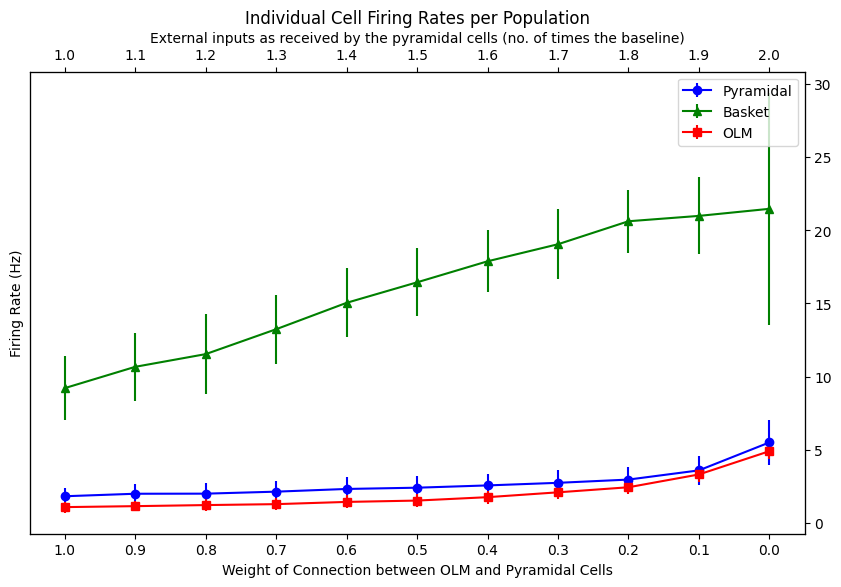
\includegraphics[width=1.0\textwidth]{Sanjay_validation_firing_rates.png}
    \caption[Validation of the firing rates]{Validation of the firing rates.}\label{fig:validation_firing_rates}
    \begin{minipage}{0.9\textwidth}
        The above figure shows the firing rates of the Pyr cells, BC cells, and O-LM cells when dendritic inhibition is decreased and external noise is increased.
        The firing rates were calculated from the spike activity of the cells in each population for the duration of the simulation (5000 ms).
        The double x-axis represents both decrement in the weight of dendritic inhibition on pyramidal cells by OLM interneurons,
        while simultaneously increasing external noise stimulation to pyramidal cells.
        External noise levels rise and inhibition decreases by increments of 0.1, each representing a 10\% change relative to the baseline.
        The y-axis represents the firing rate in Hz.
        The firing rates are per cell type: Pyr (blue), Basket (green) and OLM (red).
        The error bars represent the standard deviation of the firing rates.
    \end{minipage}
\end{figure}

\begin{figure}[htbp]
    \centering
    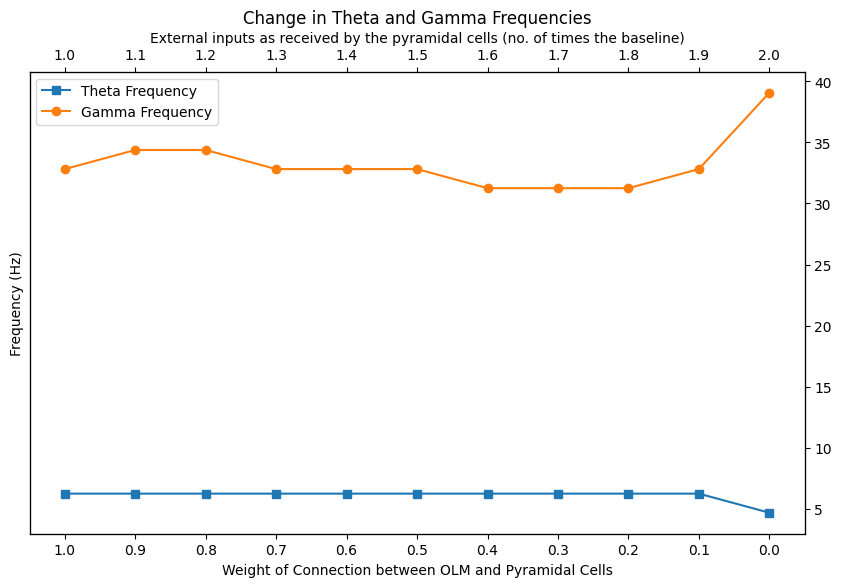
\includegraphics[width=1.0\textwidth]{Sanjay_validation_frequencies.png}
    \caption[Validation of the firing rates]{Validation of dominant frequencies.}\label{fig:validation_frequencies}
    \begin{minipage}{0.9\textwidth}
        The above figure shows the dominant theta-gamma frequencies in the network activity when dendritic inhibition is decreased and external noise is increased.
        The double x-axis represents both decrement in the weight of dendritic inhibition on pyramidal cells by O-LM interneurons,
        while simultaneously increasing external noise stimulation to pyramidal cells.
        External noise levels rise and inhibition decreases by increments of 0.1, each representing a 10\% change relative to the baseline.
        The y-axis represents the dominant frequency in Hz for both theta (3--12 Hz, blue) and gamma (30--80 Hz, orange) oscillatory bands.
    \end{minipage}
\end{figure}

\begin{figure}[htbp]
    \centering
    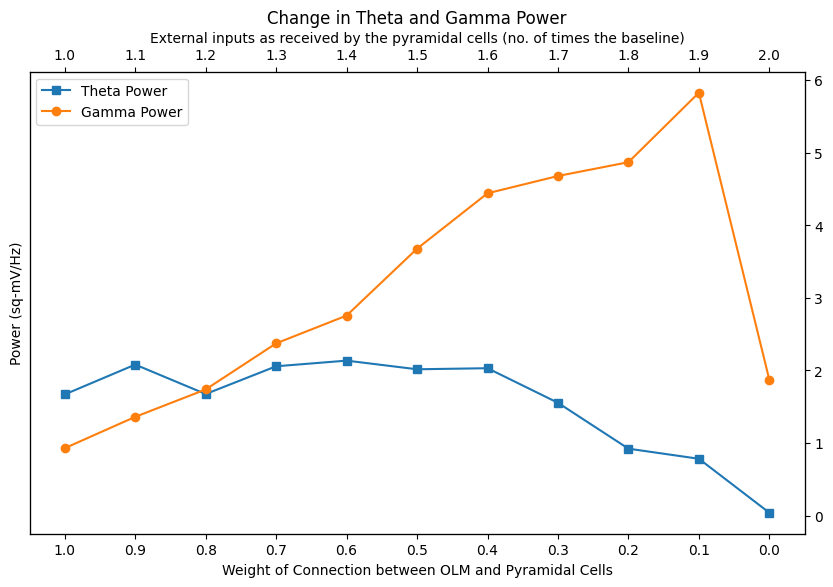
\includegraphics[width=1.0\textwidth]{Sanjay_validation_power.png}
    \caption[Validation of the firing rates]{Validation of Theta-Gamma power.}\label{fig:validation_power}
    \begin{minipage}{0.9\textwidth}
        The above figure shows the power of the theta and gamma oscillations in the network when dendritic inhibition is decreased and external noise is increased.
        The double x-axis represents both decrement in the weight of dendritic inhibition on pyramidal cells by O-LM interneurons,
        while simultaneously increasing external noise stimulation to pyramidal cells.
        External noise levels rise and inhibition decreases by increments of 0.1, each representing a 10\% change relative to the baseline.
        The y-axis represents the theta and gamma power (blue and orange, respectively).
    \end{minipage}
\end{figure}

\begin{table}[htbp]
    \centering
    \caption[Summary of Model validation: Network simulation Parameters and Results]{Overview of Model Validation Network Simulation Settings and Outcomes.
        Variations in the firing rates of cell populations, alongside theta and gamma oscillations within the local field potential, as well as the alterations in their intensity upon the decrease of dendritic inhibition and the concurrent enhancement of external stimuli to the pyramidal neurons.}\label{tab:validation_results}
    \begin{adjustbox}{width=\textwidth}
        \begin{tabular}{ccccccccc}
            \hline
            OLM-Pyr Wt & External Wt & \CellWithForcedBreak{Pyr (Hz)                                                     \\ + Std} & \CellWithForcedBreak{BWB (Hz) \\ + Std} & \CellWithForcedBreak{OLM (Hz) \\ + Std} & \CellWithForcedBreak{Theta \\ Freq (Hz)} & \CellWithForcedBreak{Theta power \\ (mV\textsuperscript{2} Hz\textsuperscript{-1})} & \CellWithForcedBreak{Gamma \\ Freq (Hz)} & \CellWithForcedBreak{Gamma power \\ (mV\textsuperscript{2} Hz\textsuperscript{-1})} \\
            \hline
            1.0X       & 1.0X        & 1.83±0.58                     & 9.21±2.20  & 1.08±0.38 & 6.2 & 1.67 & 32.8 & 0.93 \\
            0.9X       & 1.1X        & 2.00±0.64                     & 10.67±2.31 & 1.15±0.36 & 6.2 & 2.08 & 34.4 & 1.36 \\
            0.8X       & 1.2X        & 2.00±0.71                     & 11.54±2.72 & 1.22±0.39 & 6.2 & 1.67 & 34.4 & 1.74 \\
            0.7X       & 1.3X        & 2.14±0.74                     & 13.24±2.36 & 1.29±0.42 & 6.2 & 2.06 & 32.8 & 2.37 \\
            0.6X       & 1.4X        & 2.33±0.79                     & 15.04±2.35 & 1.44±0.45 & 6.2 & 2.13 & 32.8 & 2.76 \\
            0.5X       & 1.5X        & 2.41±0.80                     & 16.44±2.31 & 1.53±0.45 & 6.2 & 2.02 & 32.8 & 3.68 \\
            0.4X       & 1.6X        & 2.57±0.79                     & 17.88±2.12 & 1.76±0.45 & 6.2 & 2.03 & 31.2 & 4.44 \\
            0.3X       & 1.7X        & 2.74±0.86                     & 19.04±2.38 & 2.10±0.49 & 6.2 & 1.55 & 31.2 & 4.68 \\
            0.2X       & 1.8X        & 2.97±0.88                     & 20.61±2.14 & 2.44±0.48 & 6.2 & 0.92 & 31.2 & 4.87 \\
            0.1X       & 1.9X        & 3.59±0.99                     & 20.98±2.62 & 3.31±0.50 & 6.2 & 0.78 & 32.8 & 5.82 \\
            0.0X       & 2.0X        & 5.50±1.52                     & 21.46±7.93 & 4.90±0.52 & 4.7 & 0.04 & 39.1 & 1.87 \\
            \hline
        \end{tabular}
    \end{adjustbox}
\end{table}
\pagebreak
\section{Results of the Sodium-Potassium variants}

\todo[inline]{add some text for the firing rates plot of sodium potassium}


\begin{figure}[htbp]
    \centering
    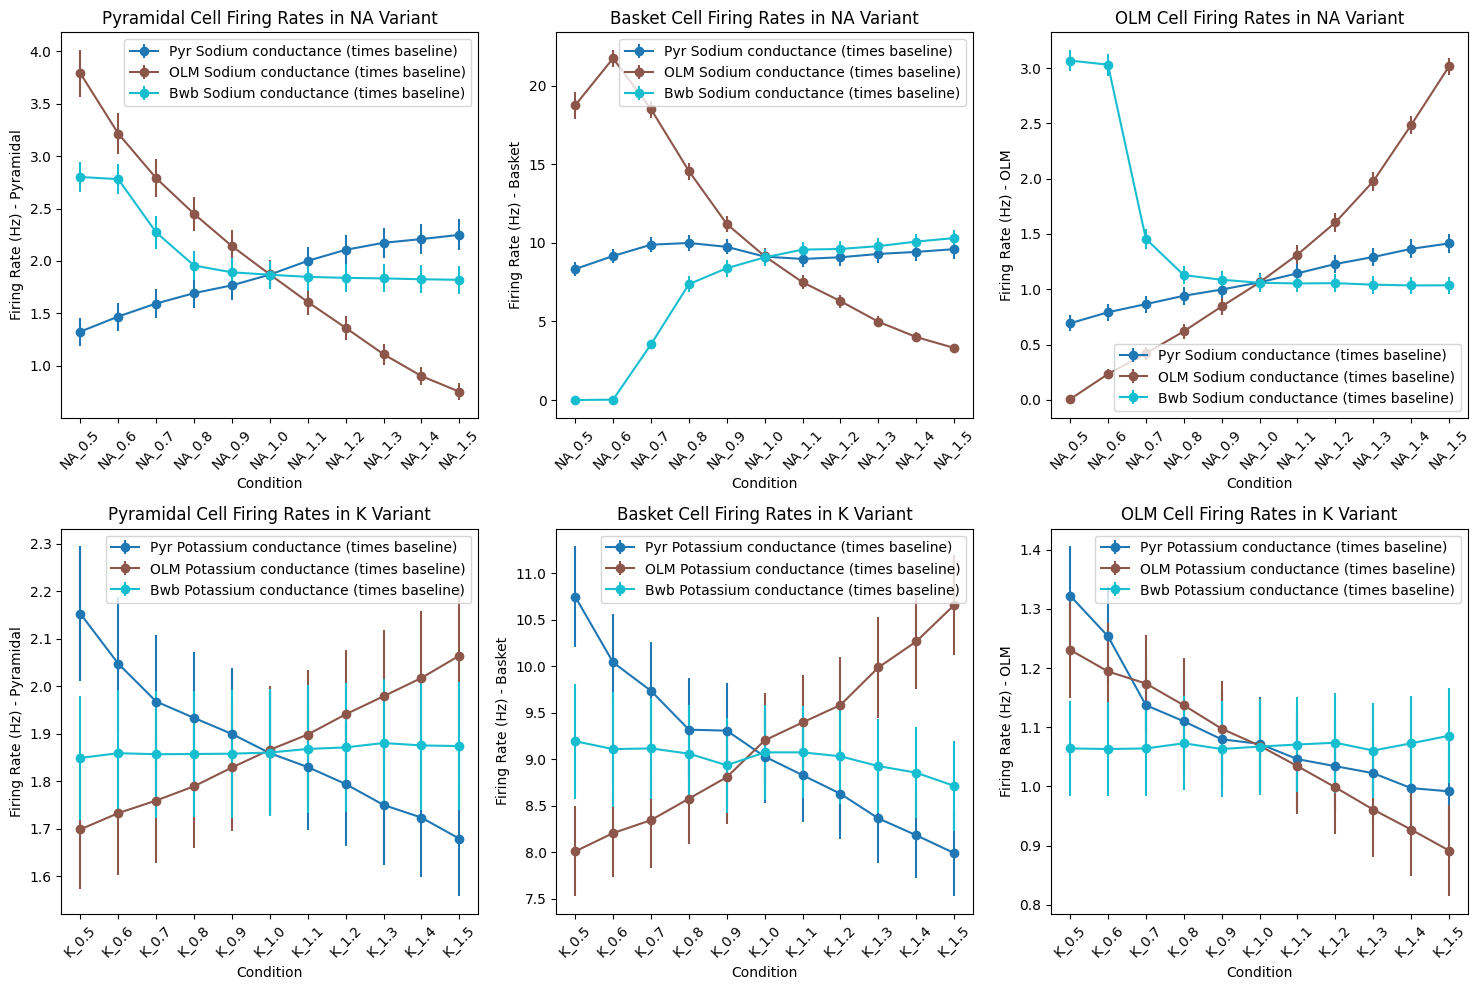
\includegraphics[width=1.0\textwidth]{Cell_firing_rates_per_pop_per_variant.png}
    \caption[Sodium-Potassium variants: Firing rates per population]{Sodium-Potassium variants: Firing rates per population.}\label{fig:sodium_potassium_firing_rates}
    \begin{minipage}{0.9\textwidth}
        The above figure shows the firing rates of the Pyr cells, BC cells, and O-LM cells for each modified cell type.
        Each of the three cell types either had modified sodium or potassium conductance.
        The firing rates were calculated from the spike activity of the cells in each population for the duration of the simulation (5000 ms).
        The x-axis represents the percentage amount of changed sodium or potassium conductance, times the baseline.
        The y-axis represents the firing rate in Hz.
        The firing rates are per cell type: Pyr (blue), Basket (cyan) and OLM (red).
        The error bars represent the standard error of the mean (SEM) of the firing rates per population.
    \end{minipage}
\end{figure}

\begin{figure}[htbp]
    \centering
    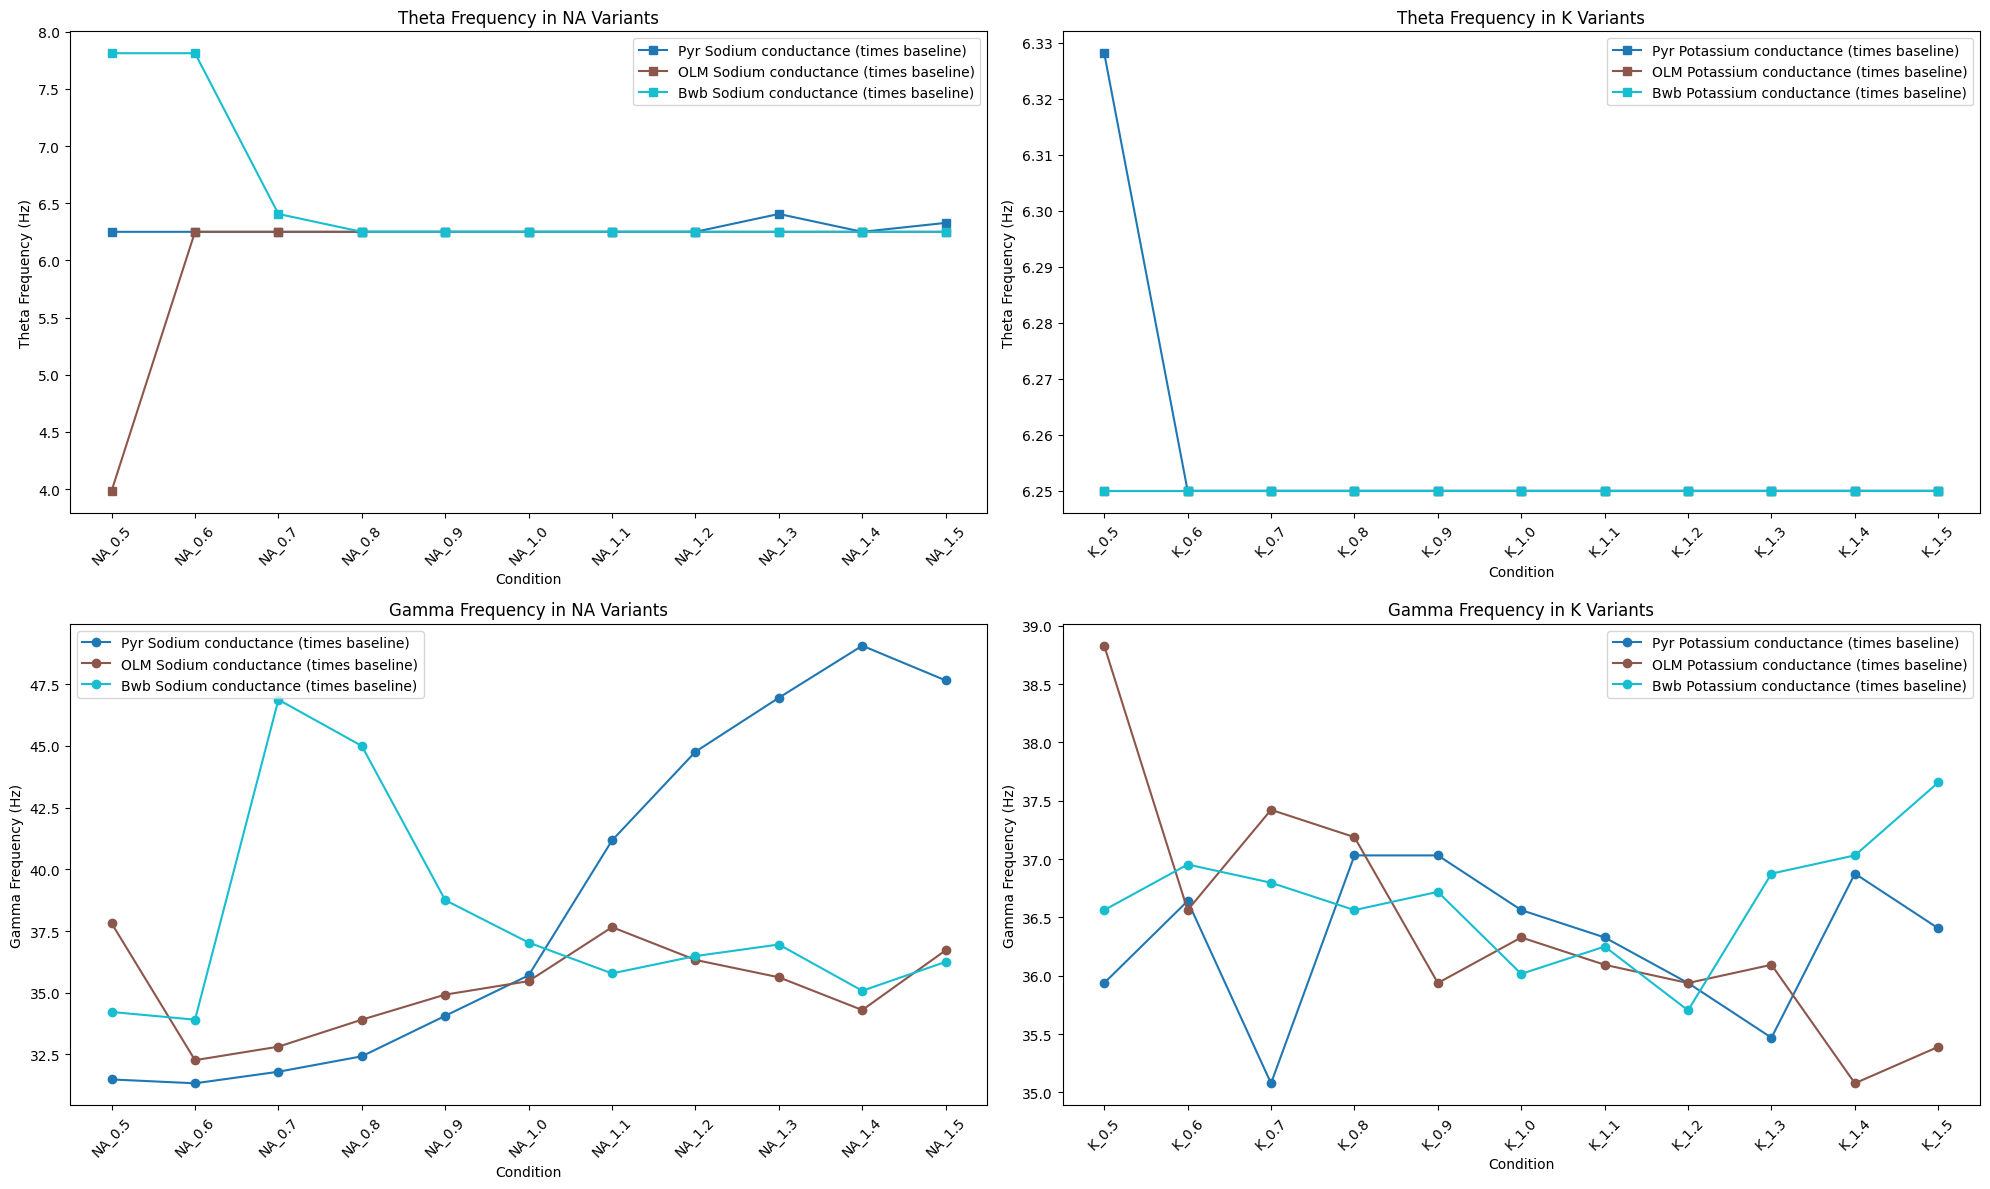
\includegraphics[width=1.0\textwidth]{Theta_gamma_freqs_variants.png}
    \caption[Sodium-Potassium variants: Dominant frequencies]{Sodium-Potassium variants: Dominant frequencies.}\label{fig:sodium_potassium_frequencies}
    \begin{minipage}{0.9\textwidth}
        The above figure shows the dominant theta-gamma frequencies in the network activity for each modified cell type.
        Each of the three cell types either had modified sodium or potassium conductance (pyr = blue, OLM = red, basket = cyan).
        The dominant frequencies were calculated from the local field potential (LFP) for the duration of the simulation (5000 ms).
        The x-axis represents the percentage amount of changed sodium or potassium conductance, times the baseline.
        The y-axis represents the dominant frequency in Hz for both theta (3--12 Hz, blue) and gamma (30--80 Hz, orange) oscillatory bands.
    \end{minipage}
\end{figure}
\begin{figure}[htbp]
    \centering
    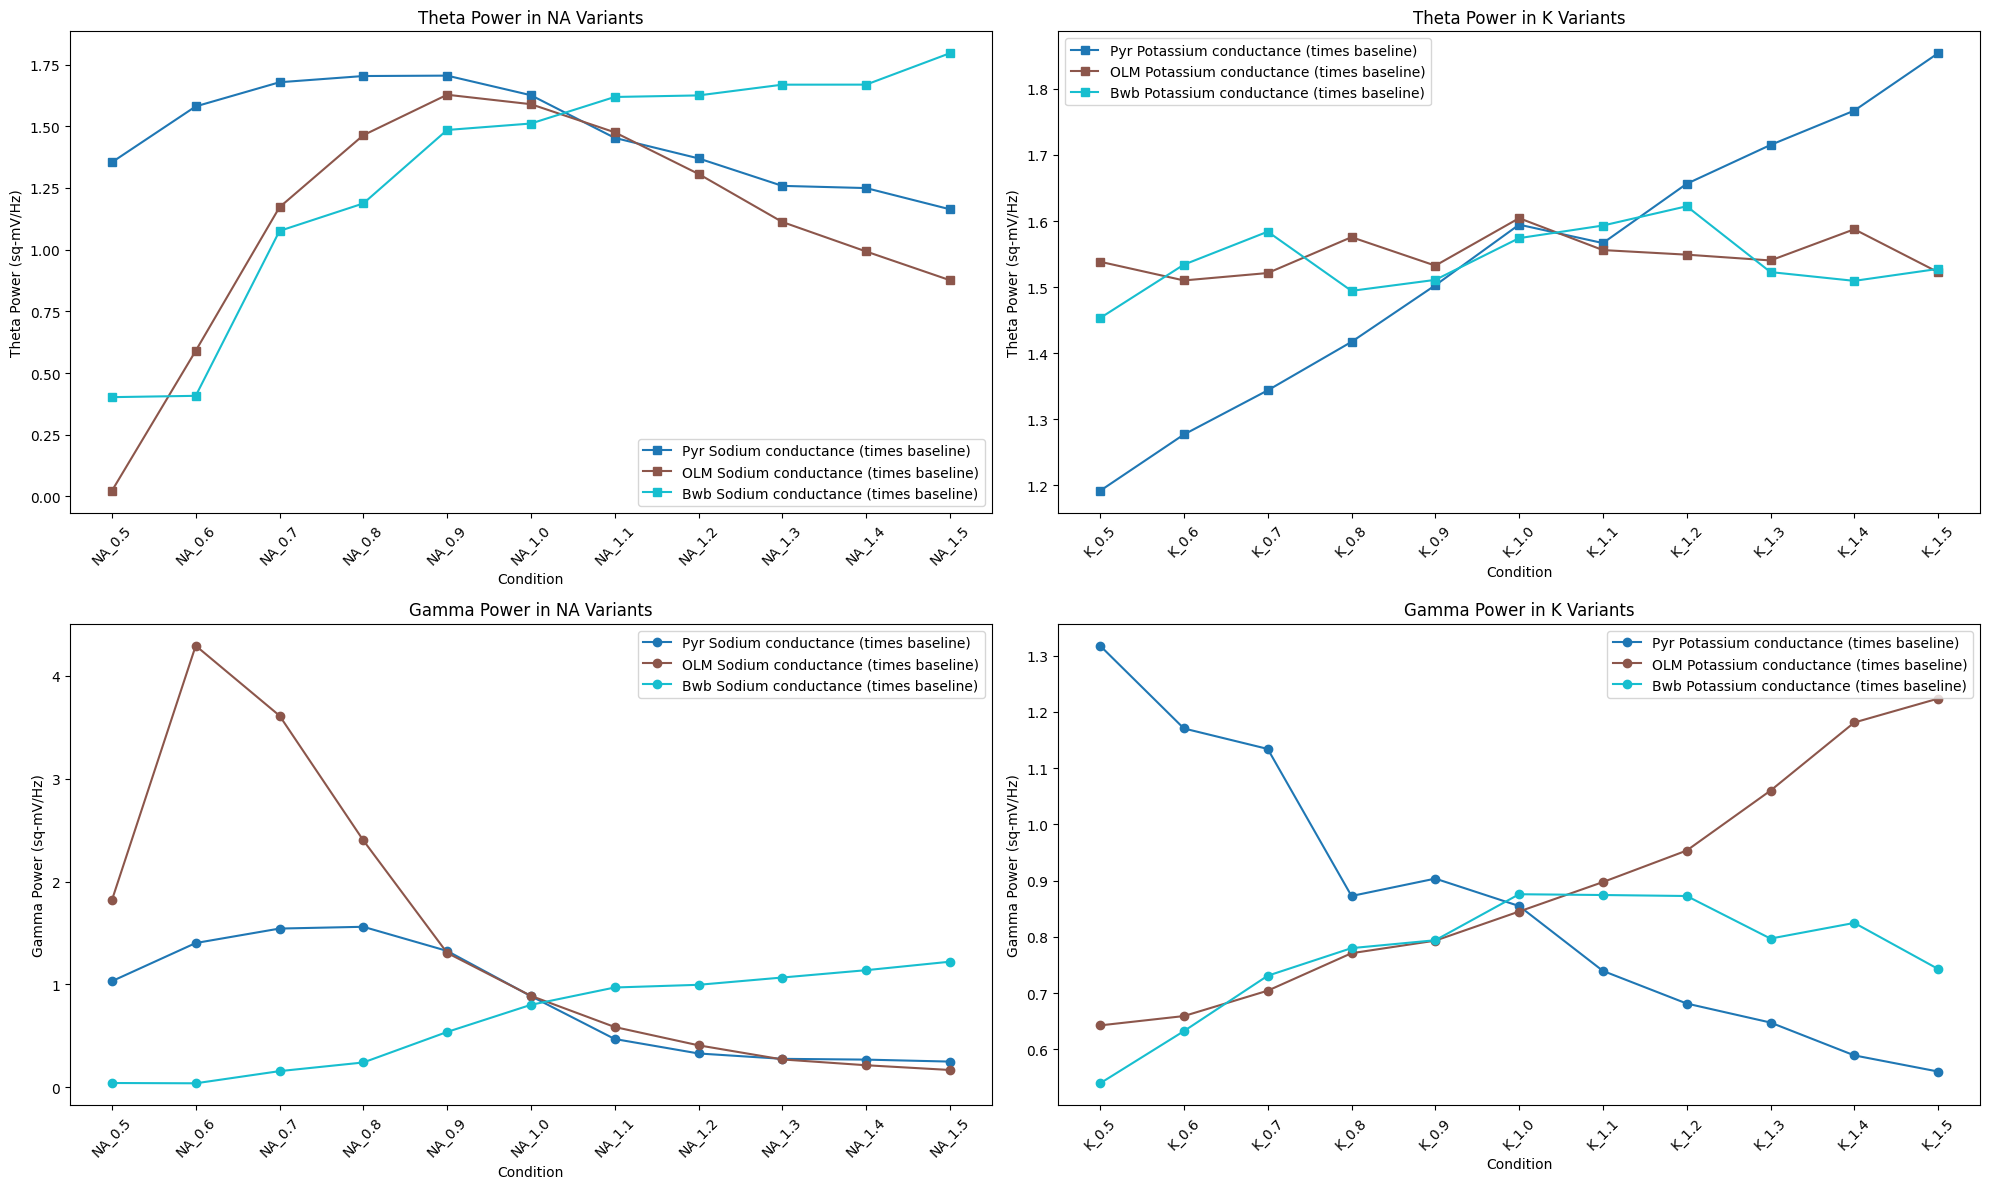
\includegraphics[width=1.0\textwidth]{Theta_gamma_power_variants.png}
    \caption[Sodium-Potassium variants: Theta-Gamma power]{Sodium-Potassium variants: Theta-Gamma power.}\label{fig:sodium_potassium_power}
    \begin{minipage}{0.9\textwidth}
        The above figure shows the power of the theta and gamma oscillations in the network for each modified cell type.
        Each of the three cell types either had modified sodium or potassium conductance (pyr = blue, OLM = red, basket = cyan).
        The power of the theta and gamma oscillations were calculated from the local field potential (LFP) for the duration of the simulation (5000 ms).
        The x-axis represents the percentage amount of changed sodium or potassium conductance, times the baseline.
        The y-axis represents the theta and gamma power (blue and orange, respectively).
    \end{minipage}
\end{figure}
\pagebreak

\section{Results of the External Noise variants}

\todo[inline]{don't forget to add some text to the previous results sections, not just captions under figures.}

\begin{figure}[H]
    \centering
    % Row 1
    \begin{subfigure}{0.48\textwidth}
        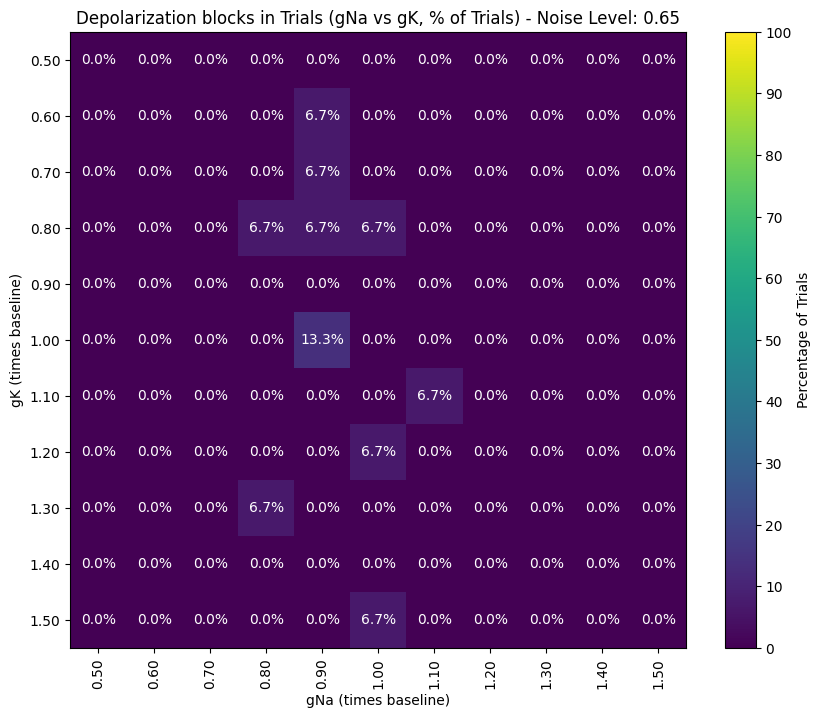
\includegraphics[width=\linewidth]{DPB_percentage_matrices/DPB_percentage_noise_0.65.png}
        \caption{} % Optional caption
    \end{subfigure}\hfill
    \begin{subfigure}{0.48\textwidth}
        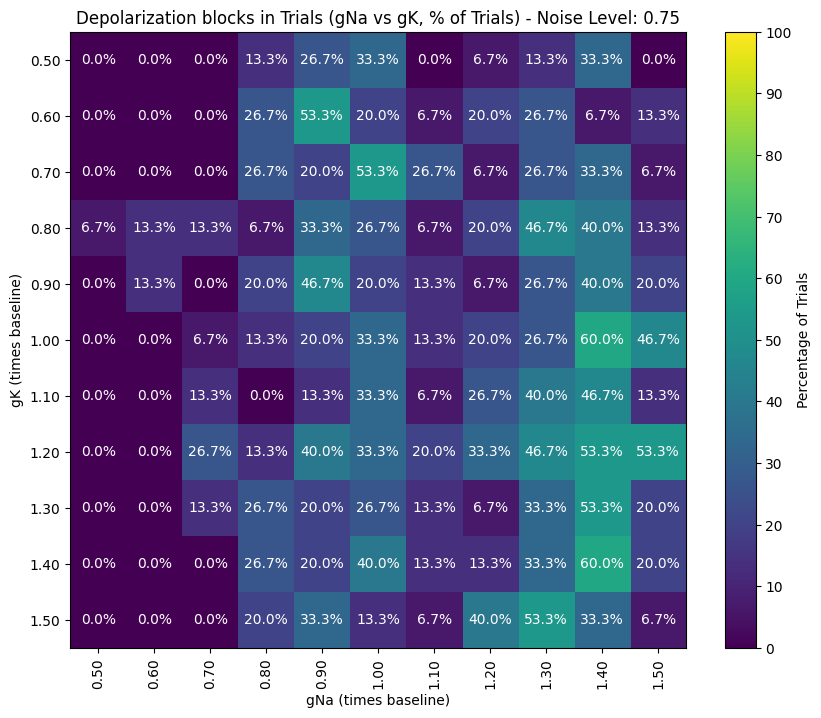
\includegraphics[width=\linewidth]{DPB_percentage_matrices/DPB_percentage_noise_0.75.png}
        \caption{} % Optional caption
    \end{subfigure}

    \bigskip % Adds vertical space between the rows

    % Row 2
    \begin{subfigure}{0.48\textwidth}
        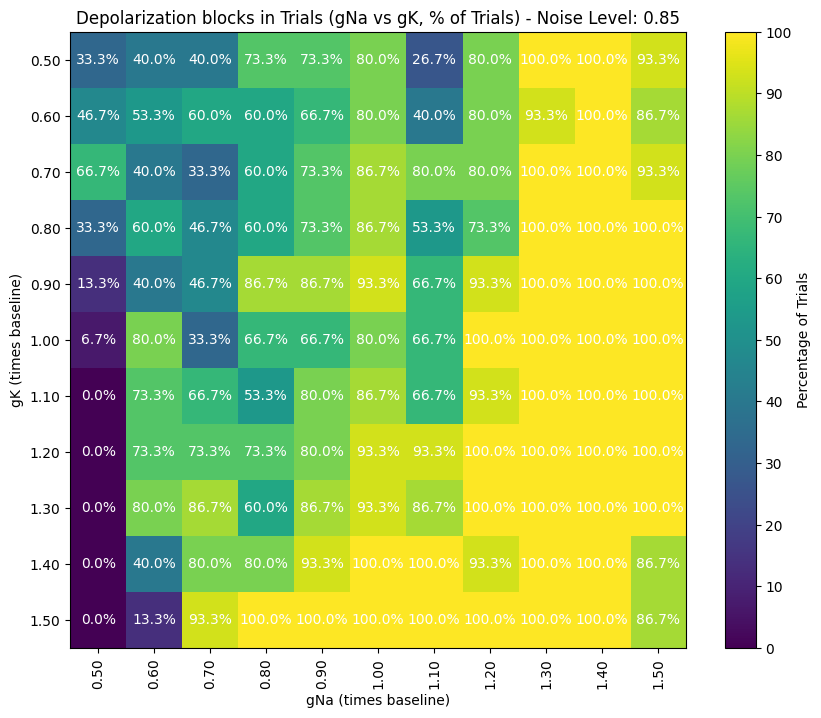
\includegraphics[width=\linewidth]{DPB_percentage_matrices/DPB_percentage_noise_0.85.png}
        \caption{} % Optional caption
    \end{subfigure}\hfill
    \begin{subfigure}{0.48\textwidth}
        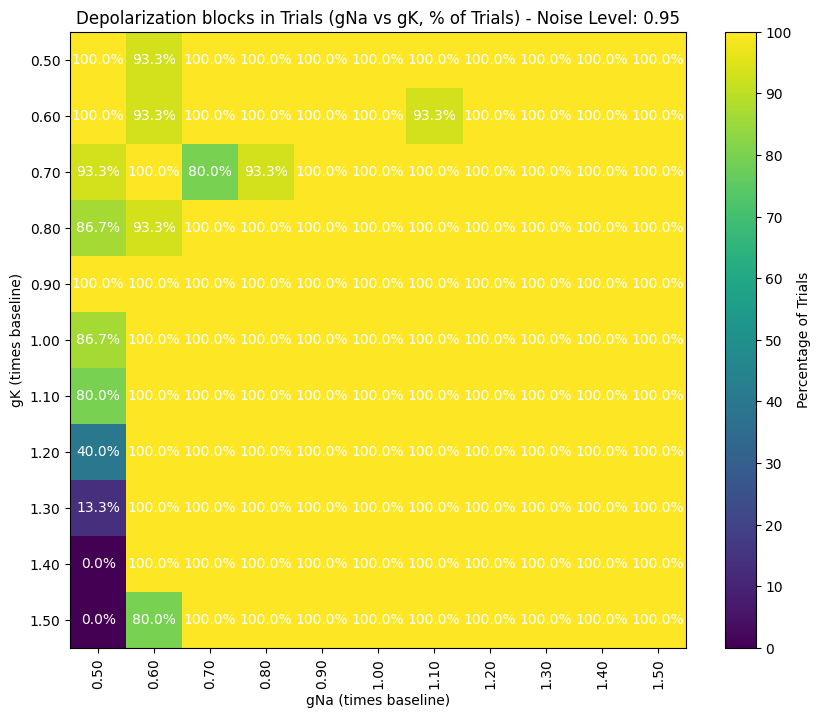
\includegraphics[width=\linewidth]{DPB_percentage_matrices/DPB_percentage_noise_0.95.png}
        \caption{} % Optional caption
    \end{subfigure}

    \caption[DPB percentage matrices]{Percentage of trials where depolarization block events occurred for all tested noise conditions.
    The x-axis shows all the sodium conductance changes in pyramidal cells, whereas the y-axis shows the potassium conductance changes in pyramidal cells.
    Modifications to pyramidal cells were applied to all compartments.
    The color intensity scales from 0 to 100 \%, where high-intensity yellow equals a higher amount of DPB events in a condition.
    The images are labeled from low noise to higher noise (a through d), respectively.}\label{fig:dpb_percentage_matrices}
\end{figure}

\begin{figure}[H]
    \centering
    % Row 1
    \begin{subfigure}{0.48\textwidth}
        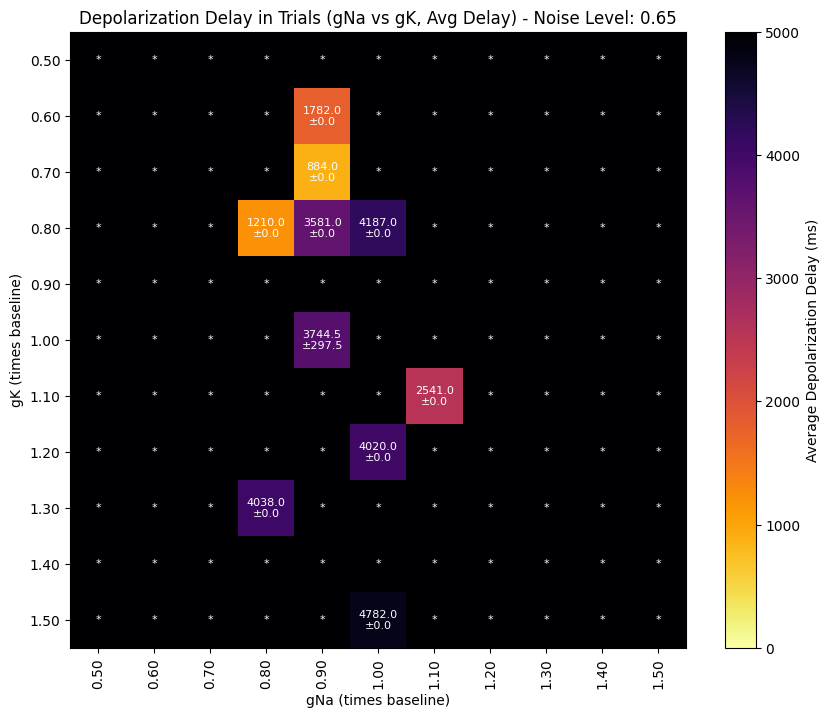
\includegraphics[width=\linewidth]{DPB_delay_matrices/DPB_delay_noise_0.65.png}
        \caption{} % Optional caption
    \end{subfigure}\hfill
    \begin{subfigure}{0.48\textwidth}
        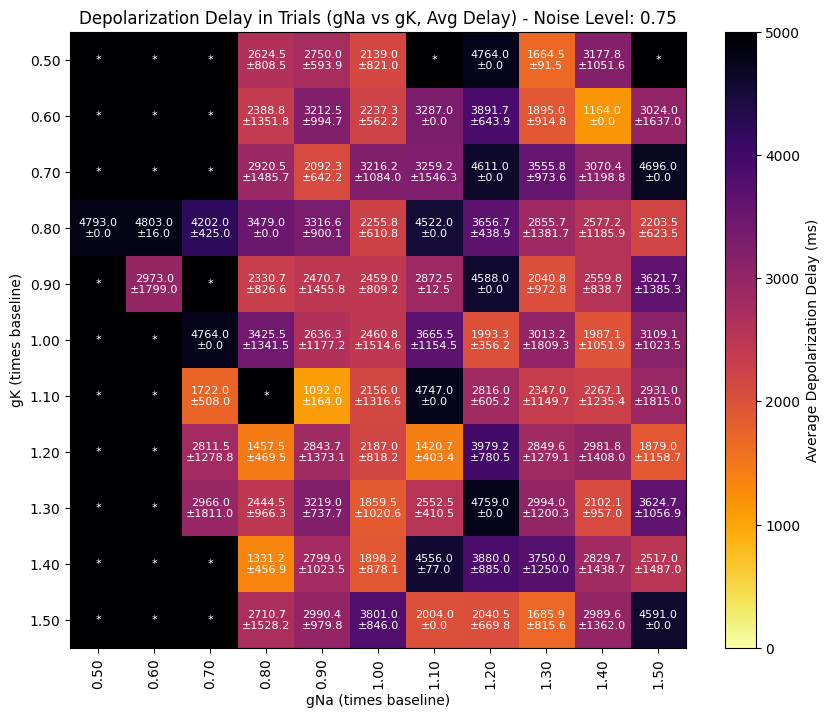
\includegraphics[width=\linewidth]{DPB_delay_matrices/DPB_delay_noise_0.75.png}
        \caption{} % Optional caption
    \end{subfigure}

    \bigskip % Adds vertical space between the rows

    % Row 2
    \begin{subfigure}{0.48\textwidth}
        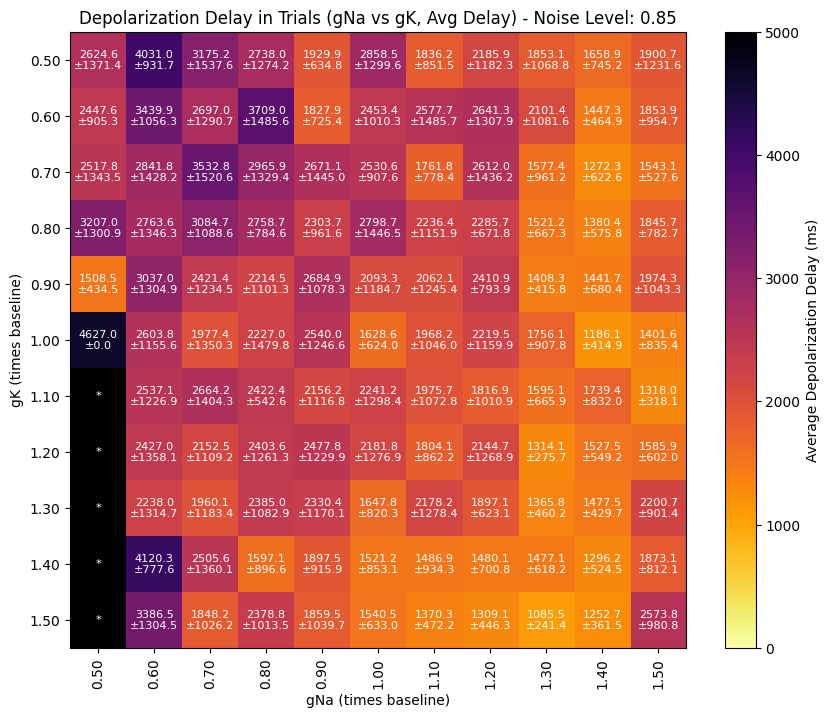
\includegraphics[width=\linewidth]{DPB_delay_matrices/DPB_delay_noise_0.85.png}
        \caption{} % Optional caption
    \end{subfigure}\hfill
    \begin{subfigure}{0.48\textwidth}
        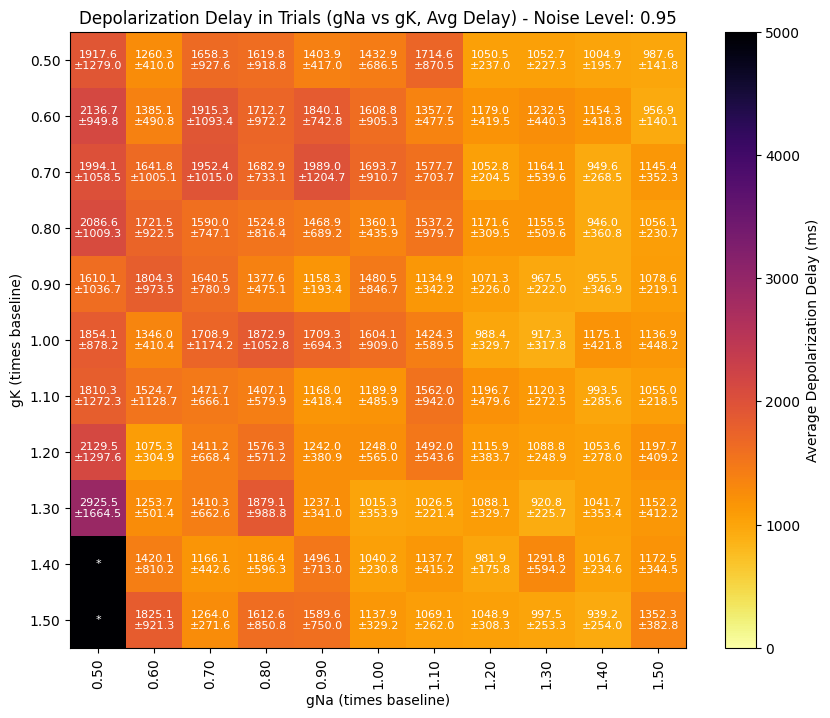
\includegraphics[width=\linewidth]{DPB_delay_matrices/DPB_delay_noise_0.95.png}
        \caption{} % Optional caption
    \end{subfigure}

    \caption[DPB delay matrices]{Average delay + Standard deviation of DPB in trials where depolarization block events occurred for all tested noise conditions.
    The x-axis shows all the sodium conductance changes in pyramidal cells, whereas the y-axis shows the potassium conductance changes in pyramidal cells.
    Modifications to pyramidal cells were applied to all compartments.
    The color intensity shows the average delay, where high-intensity red equals a shorter delay in DPB events in a condition.
    The images are labeled from low noise to higher noise (a through d), respectively.}\label{fig:dpb_delay_matrices}
\end{figure}
\pagebreak
\section{Results of the External Noise: Burst analysis}
% First page with 3 sub-figures
\begin{figure}[!htb]
    \centering
    % First sub-figure
    \begin{subfigure}{\textwidth}
        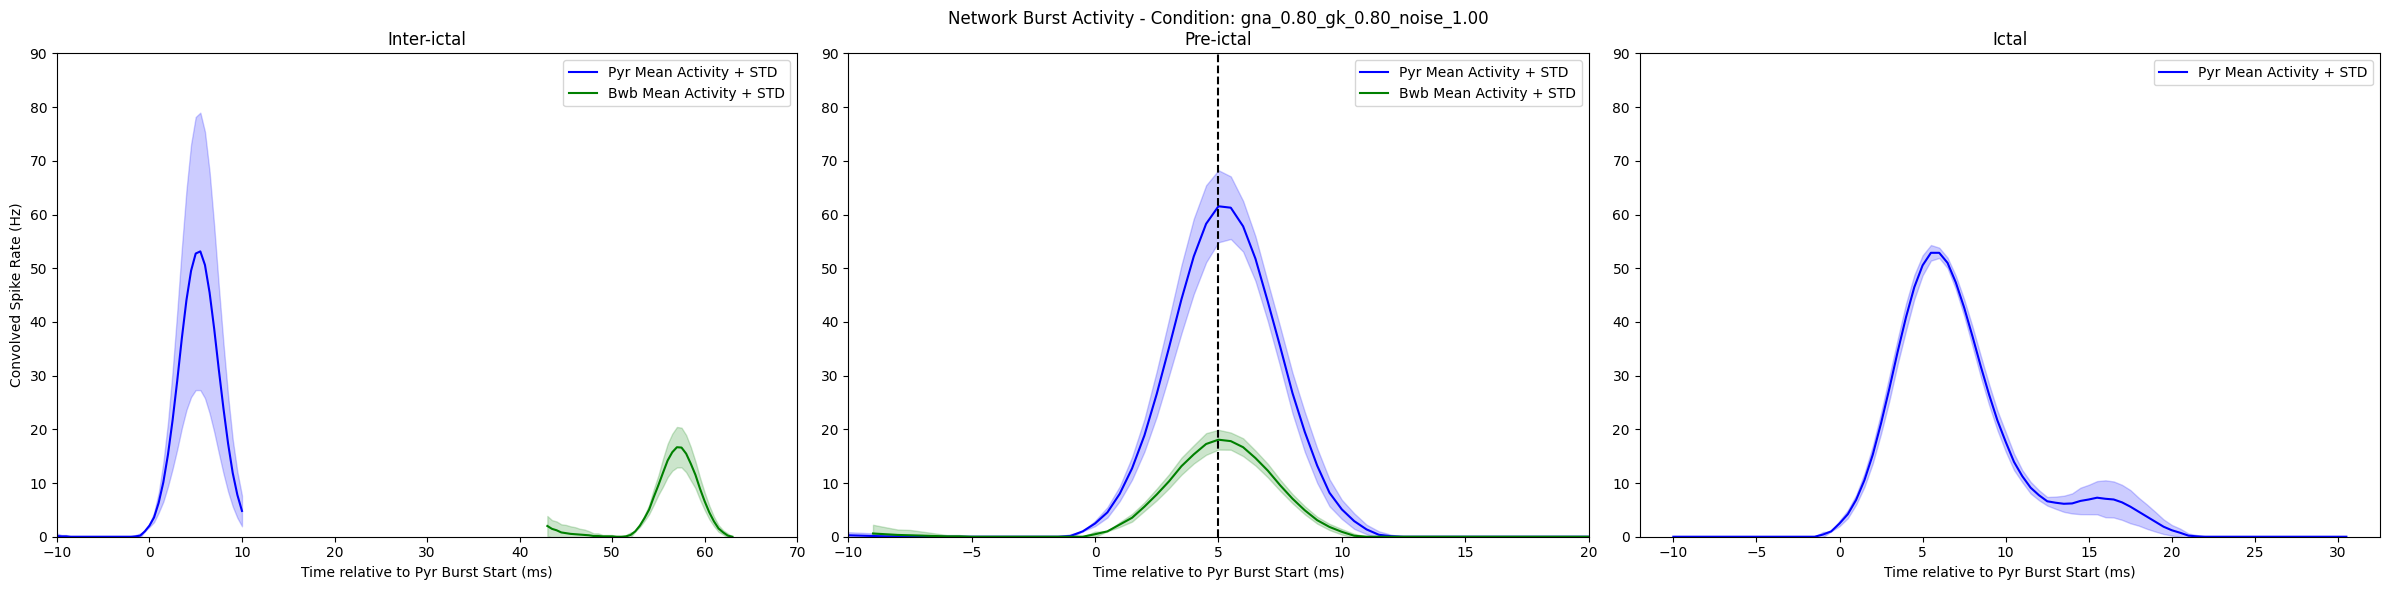
\includegraphics[width=\linewidth]{network_activity_0.80_0.80_1.00.png}
        \caption{} % Optional caption or label
    \end{subfigure}
    \vspace{1em} % Space between the sub-figures

    % Second sub-figure
    \begin{subfigure}{\textwidth}
        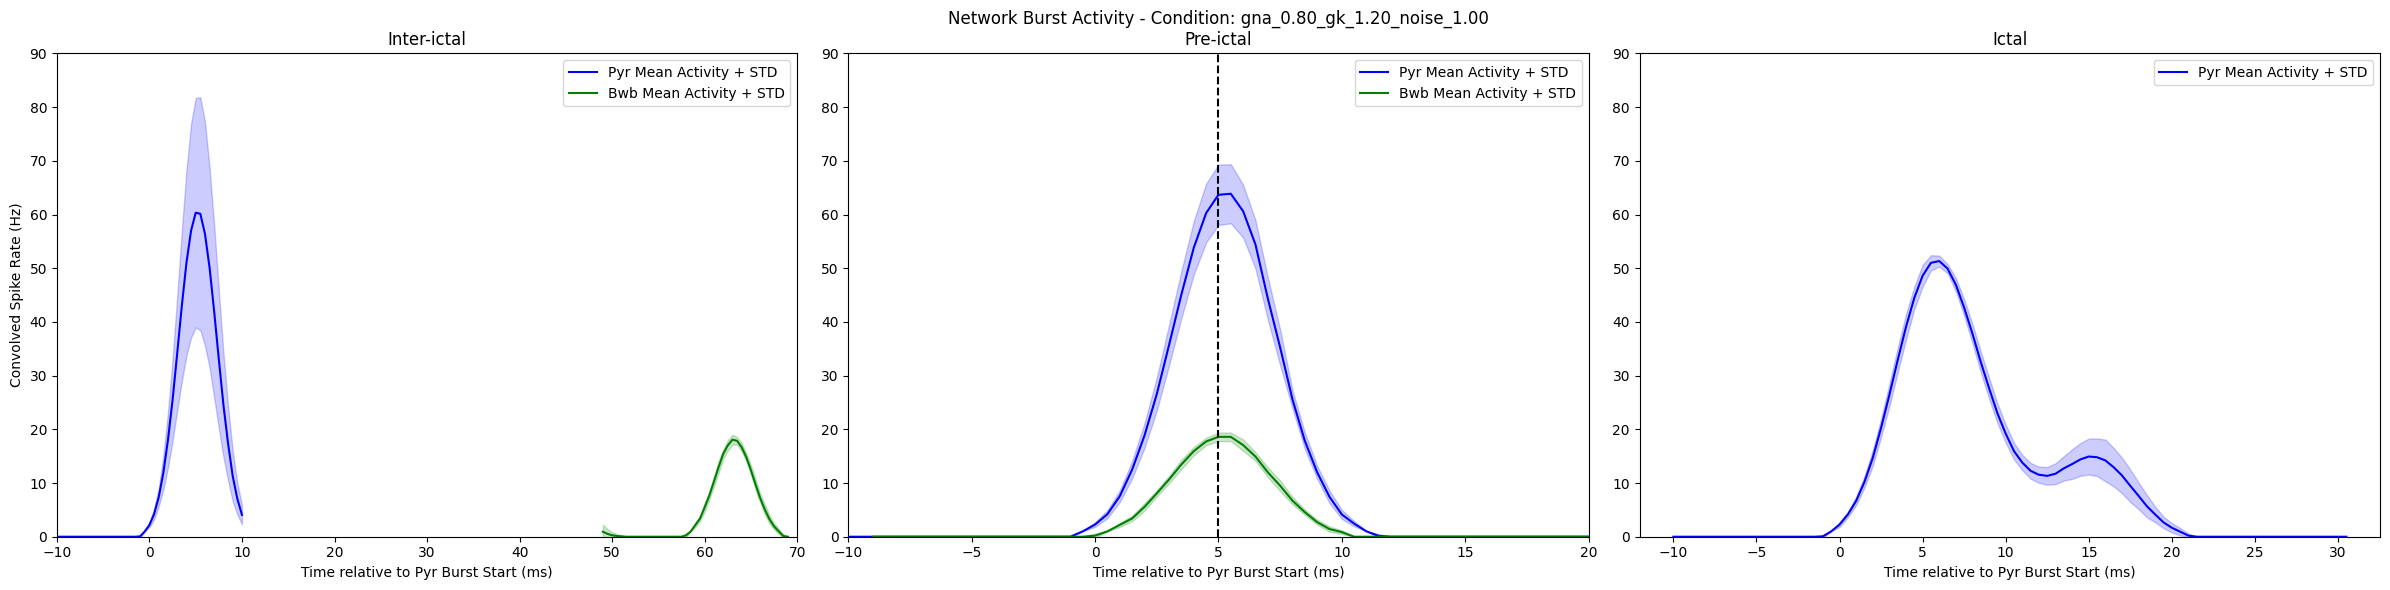
\includegraphics[width=\linewidth]{network_activity_0.80_1.20_1.00.png}
        \caption{} % Optional caption or label
    \end{subfigure}
    \vspace{1em} % Space between the sub-figures

    % Third sub-figure
    \begin{subfigure}{\textwidth}
        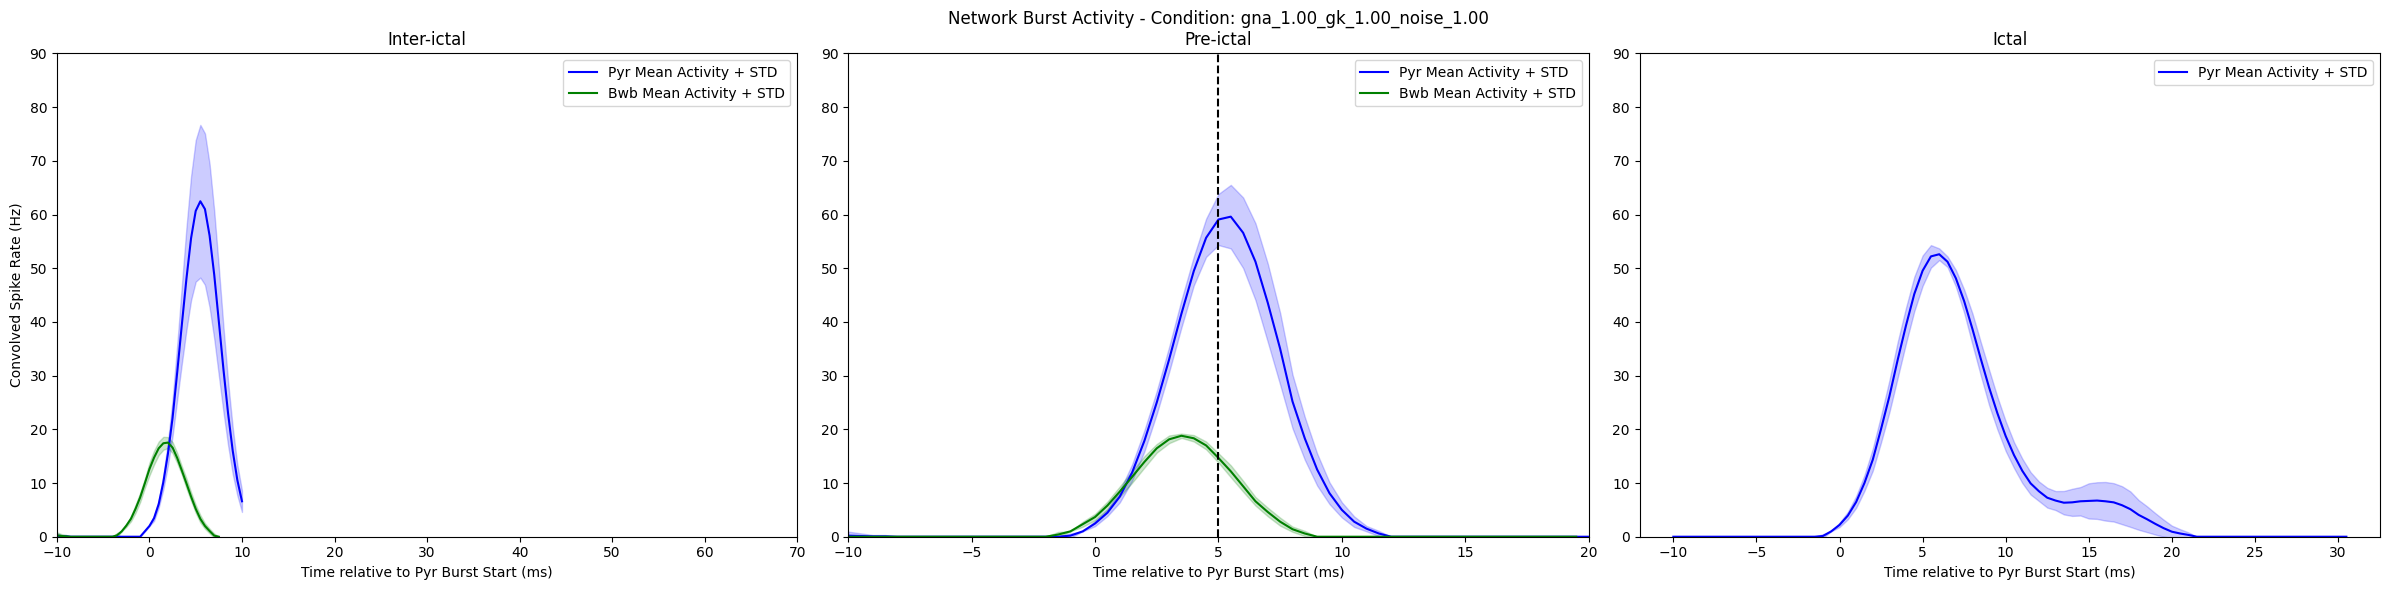
\includegraphics[width=\linewidth]{network_activity_1.00_1.00_1.00.png}
        \caption{} % Optional caption or label
    \end{subfigure}

    \caption{Burst detection near the onset of the depolarization block. Shows the 2nd to last burst before the DPB (inter-ictal, left), 
    the last burst before the DPB (pre-ictal, middle), and the first burst after the DPB (ictal, right). 
    The bursts are aligned relative the the onset of the burst of the pyramidal population in the network (ms). 
    The curve of the spike burst shows the standard deviation of the spike activity as a filled gradient surrounding the curve. 
    The bursts of both pyramidal neurons (blue) and basket cells are shown (green).}\label{fig:burst_detection}
\end{figure}
\clearpage % Ensure the continuation starts on a new page

% Second page with 2 sub-figures continued
\begin{figure}[!htb] \ContinuedFloat% Continue the figure from the previous page
    \centering
    % Fourth sub-figure
    \begin{subfigure}{\textwidth}
        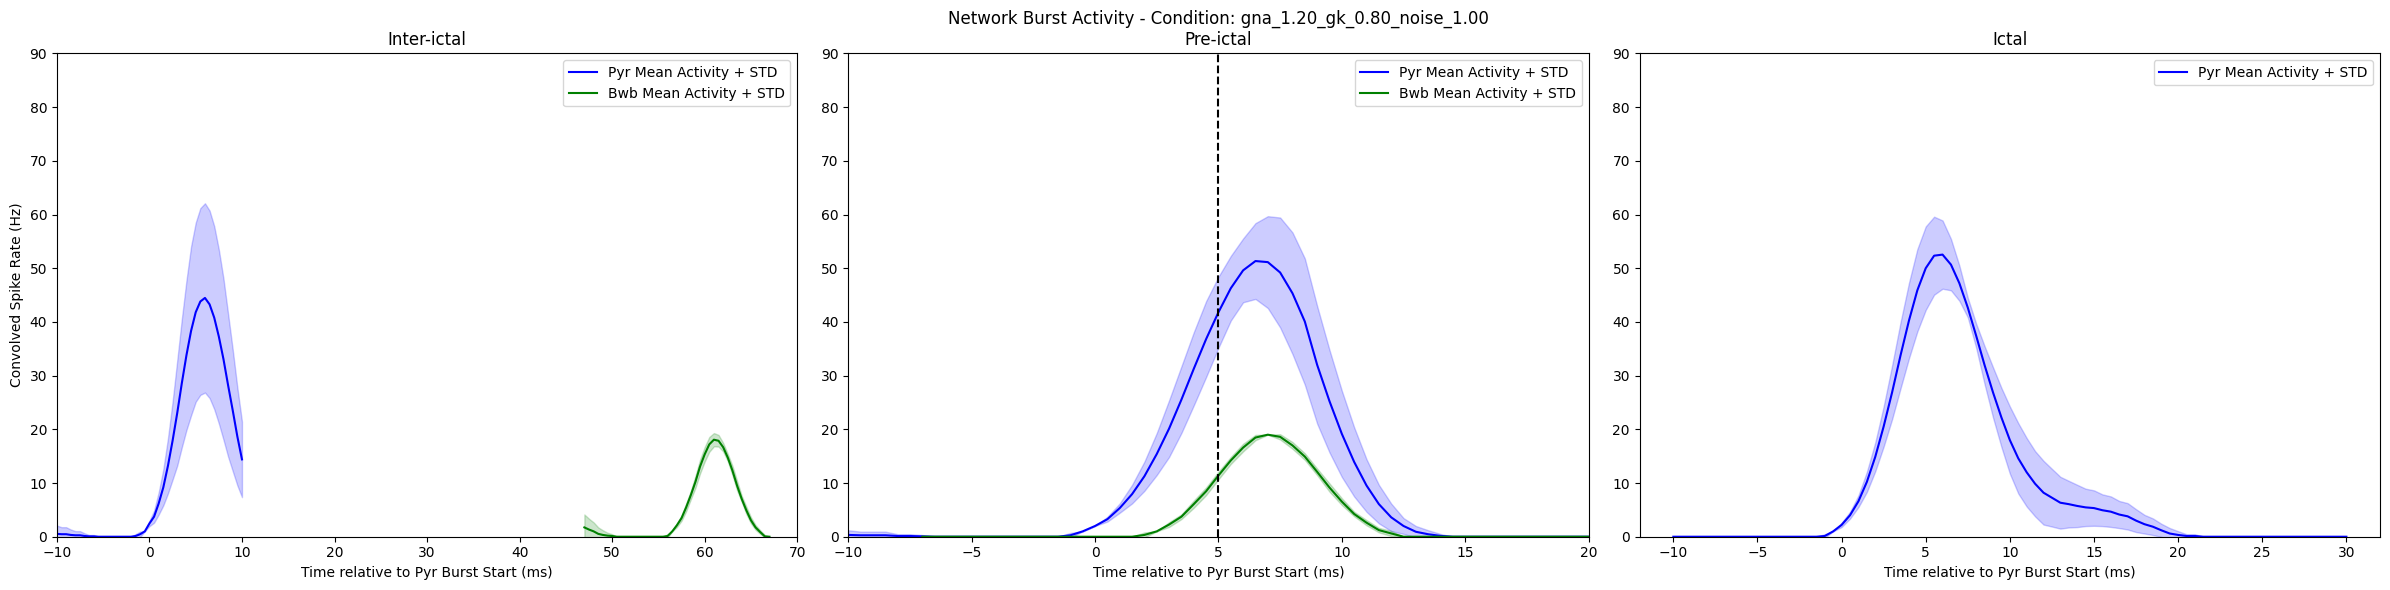
\includegraphics[width=\linewidth]{network_activity_1.20_0.80_1.00.png}
        \caption{} % Optional caption or label
    \end{subfigure}
    \vspace{1em} % Space between the sub-figures

    % Fifth sub-figure
    \begin{subfigure}{\textwidth}
        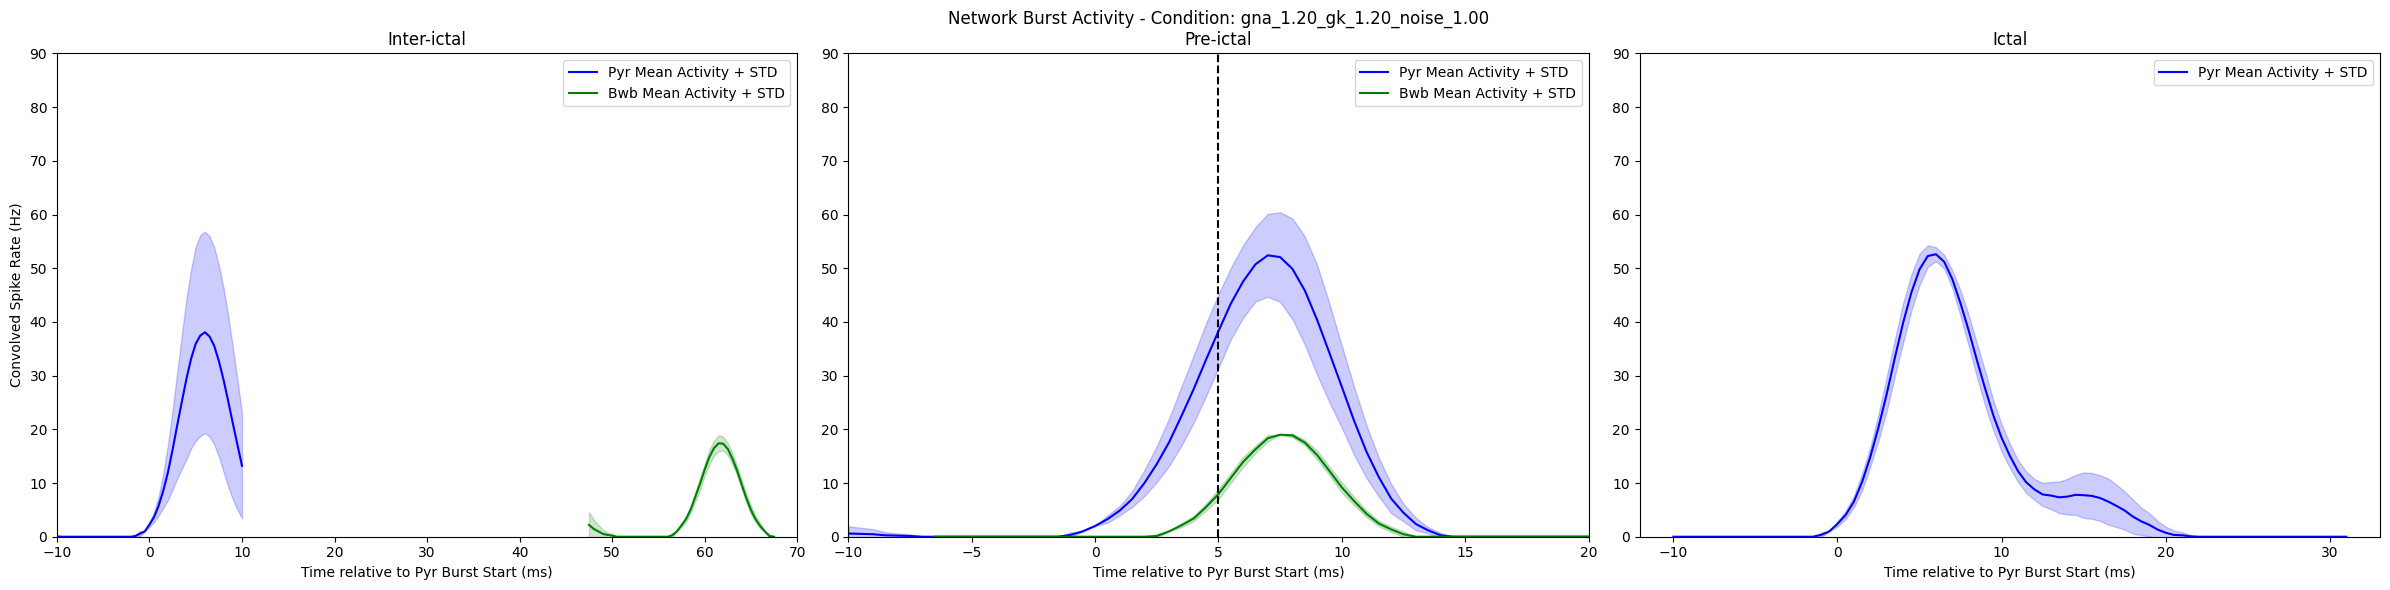
\includegraphics[width=\linewidth]{network_activity_1.20_1.20_1.00.png}
        \caption{} % Optional caption or label
    \end{subfigure}

    % No need for a new caption or label; it's a continuation
\end{figure}

\section{Results of the Recurrent Connections variants}
\begin{figure}[H]
    \centering
    % Row 1
    \begin{subfigure}{0.48\textwidth}
        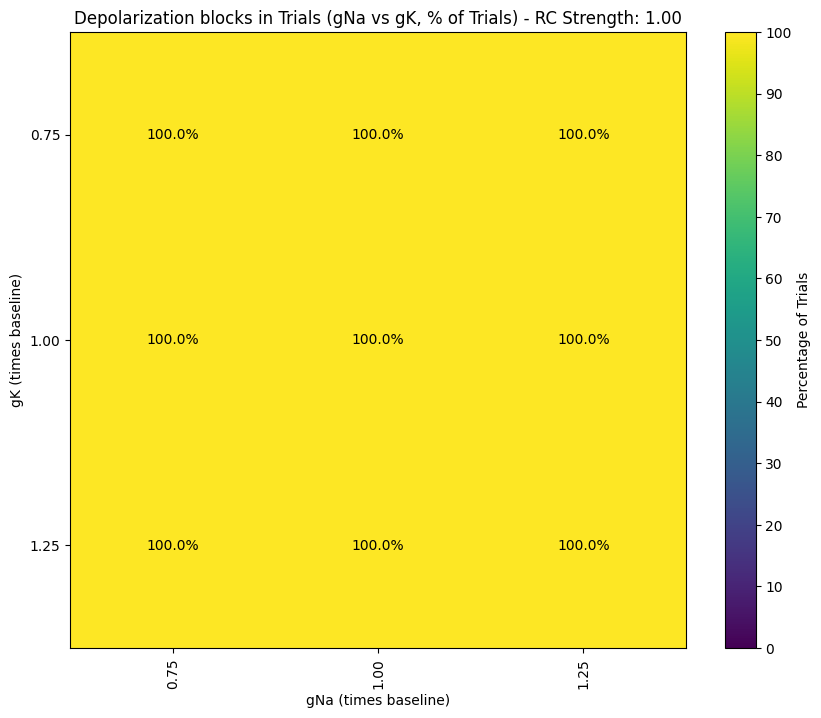
\includegraphics[width=\linewidth]{DPB_RC_Percentages/DPB_percentages_RC_1.00.png}
        \caption{} % Optional caption
    \end{subfigure}\hfill
    \begin{subfigure}{0.48\textwidth}
        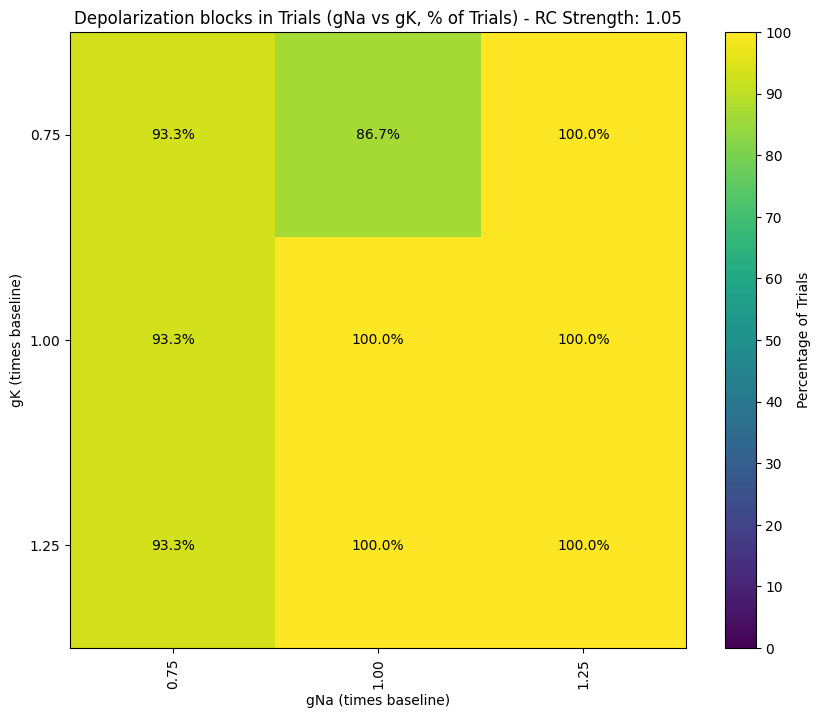
\includegraphics[width=\linewidth]{DPB_RC_Percentages/DPB_percentages_RC_1.05.png}
        \caption{} % Optional caption
    \end{subfigure}

    \bigskip % Adds vertical space between the rows

    % Row 2
    \begin{subfigure}{0.48\textwidth}
        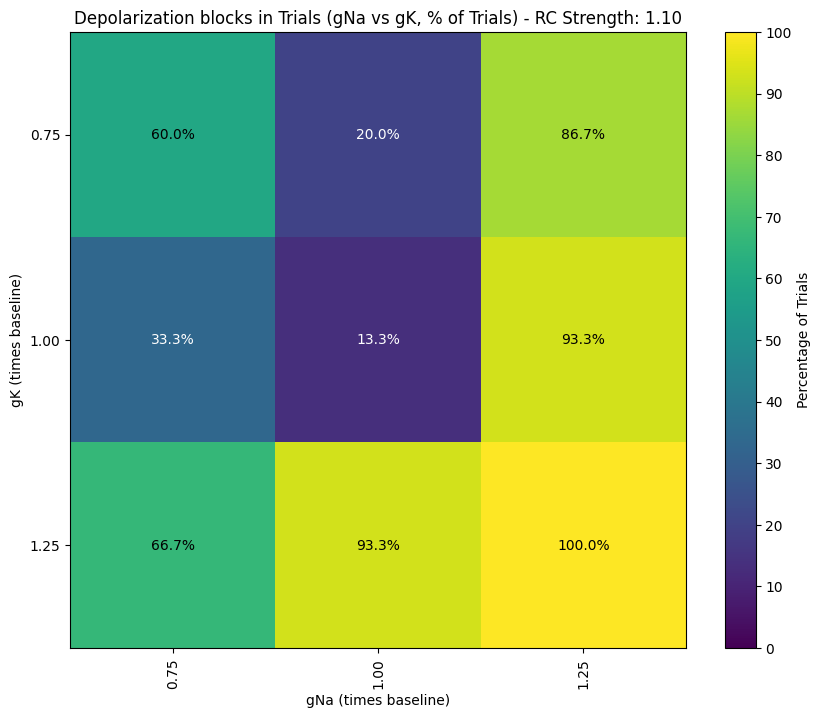
\includegraphics[width=\linewidth]{DPB_RC_Percentages/DPB_percentages_RC_1.10.png}
        \caption{} % Optional caption
    \end{subfigure}\hfill
    \begin{subfigure}{0.48\textwidth}
        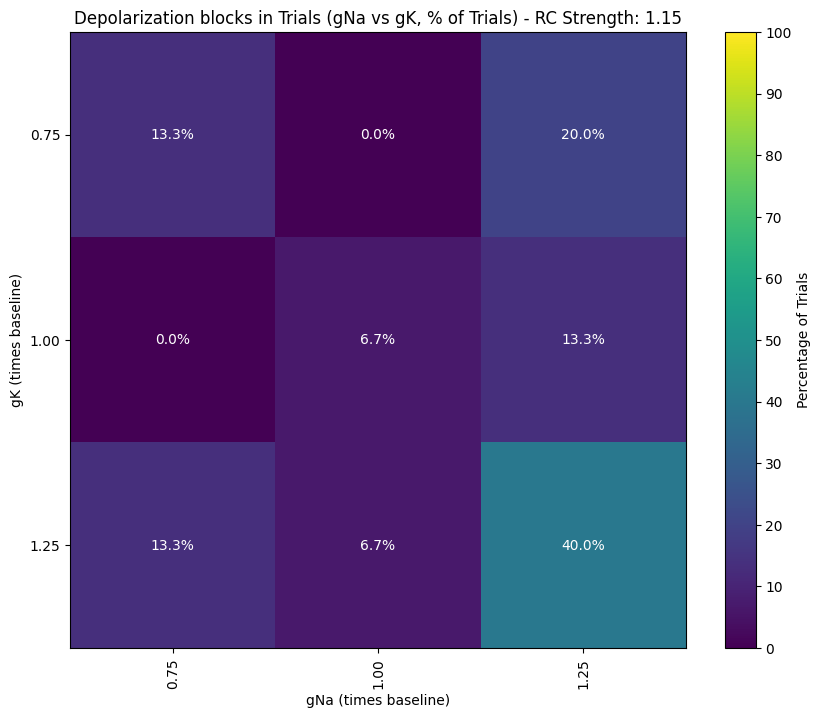
\includegraphics[width=\linewidth]{DPB_RC_Percentages/DPB_percentages_RC_1.15.png}
        \caption{} % Optional caption
    \end{subfigure}

    \caption[RC DPB percentage matrices (all)]{Percentage of trials where depolarization block events occurred for all tested noise conditions.
        The x-axis shows all the sodium conductance changes in pyramidal cells, whereas the y-axis shows the potassium conductance changes in pyramidal cells.
        Modifications to pyramidal cells were applied to all compartments.
        The color intensity shows the average delay, where high-intensity yellow equals higher percentage of DPB events in a condition.
        The images are labeled from low noise to higher noise (a through d), respectively.}\label{fig:rc_dpb_percentage_matrices}
\end{figure}
\chapter{Discussion}

This study used a computer model of the CA3 subfield of the hippocampus originally developed by \textcite{neymotinKetamineDisruptsTheta2011}.
This model was used to study the effects of several different parameters that could initiate an epileptic state.

Initially, the implementation of the baseline model was verified to ensure that the model was functioning as expected.
Similar metrics, to the ones tested in the adaptation by \textcite{sanjayImpairedDendriticInhibition2015} were used to verify the model.
These metrics included population firing rates and theta-gamma oscillations (power and frequency).
The experiments by \textcite{sanjayImpairedDendriticInhibition2015} explored the effects of impaired dendritic inhibition in the CA3 network
as the main cause of epilepsy in the highly vulnerable brain region that is the CA3 subfield.

The results of our baseline model were consistent with the results of the \textcite{sanjayImpairedDendriticInhibition2015} study,
which made it possible to proceed with variations and additional experiments using the same CA3 model in NEURON simulator.

First, the network dynamics due to dysfunctional voltage-gated ion channels for sodium and potassium
were investigated in pyramidal, basket and O-LM cells populations within a CA3 hippocampal network.
These variations of channel dynamics (conductance) were simulated to resemble epileptic genetic profiles which could be related TLE patients.

In addition to that, the networks susceptibility to external noise was tested by varying the noise level in the network with similar channel dynamics.
Per trial of a condition, the amount of occurrences of depolarization blocks in the basket cell populations were counted and the average delay in the
loss in basket cell activity was calculated.

Lastly, it was explored if the network could be rescued from an epileptic state by gradually increasing the strength of soma inhibition by basket cells
by increasing the weight of recurrent connection within the basket cell population. Again, counting the amount of occurrences of depolarization blocks
in the basket cell populations.
\pagebreak

\section{Model assumptions and Observations}
In the original experiments \textcite{sanjayImpairedDendriticInhibition2015} the authors studied if impaired dendritic
inhibition could lead to epileptic activity in the network.
In their three experiment scenario's, they impaired the dendritic inhibition by O-LM cells on pyramidal cells (1), increased external noise to distal
dendrites of pyramidal cells (2), and modified the connection strength of all cell types in the network (3).
Their findings had no previous experimental validation and a linear relationship was assumed.

In this study, the experiments build upon the observations made by \textcite{sanjayImpairedDendriticInhibition2015} and further explored the network dynamics.
Simulations were done separately, with step-wise modifications to parameters such as conductance or connection weight.
This was necessary in order to be able to determine the extent in which these parameters could potentially lead to epileptic activity.

In all experiments Medial Septum inputs were kept constant at 150 ms intervals to both O-LM and basket cell populations
and simulations ran for 5 seconds in each trial for consistency.

\subsection{Sodium and Potassium variants}
In the first experiment, sodium and potassium conductance parameters were modified
in each cell type separately to identify which population had the most influence
on firing activity of the other cell types and on the theta-gamma oscillations.

\subsubsection{Pyramidal cells}
In the case of pyramidal cells, modifications to sodium in O-LM cells had the most
significant effect on their firing rate (figure~\ref{fig:sodium_potassium_firing_rates}, left). Similarly to directly
reducing dendritic inhibition via modification of connection weight as in scenario 1 of the \textcite{sanjayImpairedDendriticInhibition2015},
the pyramidal cells showed increased activity in their activity as (\(g_{\text{Na}}\)) for O-LM cells was reduced.
This also increased the firing rates of the other two cell types, as they receive inputs from the
pyramidal cells (figure~\ref{fig:model_design}). The large increase in basket cell firing rate directly influenced
the gamma component of the LFP (figure~\ref{fig:sodium_potassium_power}), while O-LM reduced the theta component.
These findings are consistent with the results of the \textcite{sanjayImpairedDendriticInhibition2015} study.

Out of all the cell types, pyramidal cells show the most linear relationship between the conductance of sodium
and potassium channels and their firing rate. Potassium had an oppositely proportional effect on the firing rate of
pyramidal cells compared to sodium. This result is somewhat unsurprising considering the role of potassium. In normal action potential
dynamics, voltage-dependent sodium current rapidly depolarizes the membrane via voltage-gated ion channels. As a response so too are
voltage-activated potassium channels activated that hyperpolarize the membrane potential. This effect inactivates sodium channels
as the membrane potential goes back to its polarized resting state, which in turn tunes down the firing frequency as observed.

\subsubsection{Basket cells}
In the basket cells a similar trend is visible, although the firing rate shift is much more pronounced for both modified ions.
Again, this is a sensible result, considering the fast acting GABAergic inhibitory role as an interneuron~\parencite{wangGammaOscillationSynaptic1996}.
In addition, basket cells contain extensive axonal arborization that allow them to form many connections with pyramidal cells and
to other interneurons~\parencite{tukkerDistinctDendriticArborization2013}. Especially, their many connections to cells of their own type,
might result in highly synchronized firing patterns that were observed in the population activity (figure~\ref{fig:scatterplot_20_con_olm_pyr}).
This effect is also expressed in the model, through the many-to-one connection design of the basket cells (Table~\ref{tab:bwb_gaba_connections}).

\subsubsection{O-LM cells}
O-LM cells had again somewhat linear, but relative small impact on the firing rates.
Potentially, these effects are dependent on the morphology of the O-LM cells.
O-LM cells primarily target the distal dendrites of pyramidal cells in the stratum lacunosum moleculare.
This targeting influences their firing properties, as the distal dendritic locations typically receive inputs that are less intense or
less frequent compared to the somatic or proximal dendritic inputs received by basket cells. Additionally, O-LM cells have less extensive
local axonal arborizations compared to basket cells, which limits their range of influence and the synaptic inputs they receive~\parencite{saragaActiveDendritesSpike2003}.

The primary role of O-LM cells is to modulate the input to the hippocampus from the entorhinal cortex,
affecting the integration of cortical information~\parencite{leaoOLMInterneuronsDifferentially2012}. This modulation often requires precise,
but less frequent, inhibition compared to the broad, fast inhibition exerted by basket cells on the pyramidal cell bodies.
Therefore, their activity is more phasic or conditional, dependent on specific synaptic events that do not necessitate high-frequency firing.

\subsubsection{Theta-gamma oscillations}
Interestingly, theta remains relatively stable across all cell types, while gamma oscillations are more affected by the conductance modifications.
Like in the original studies using the same model by \textcite{sanjayImpairedDendriticInhibition2015,neymotinKetamineDisruptsTheta2011},
theta is resilient to changes in the network. This resilience is mostly due to the strong pacing which is provided to the interneurons by the MS\@.
For sodium, while the theta component of the LFP appears to change a lot per condition, they are a factor 10 times smaller than does observed in the gamma component.
With potassium modifications however, only the pyramidal cells seem to resemble a linear relationship with the theta power compared to the other cell types.

Potassium conductance influences the speed at which the membrane potential returns to its resting state.
In the case of the the studied network, increased potassium conductance potentially causes faster repolarization of action potentials.
This can shorten the duration of individual spikes and reduce the overall excitability of pyramidal cells, leading to a lower firing rate.
However, this rapid repolarization can also allow neurons to return more quickly to a state where they can fire again, potentially aiding in
synchronization~\parencite{mysinMechanismsFunctionsRole2022}.
Alternatively, The quick recovery of neurons to their resting or near-threshold state can facilitate better phase-locking among neurons within
the network~\parencite{leungPhasicModulationHippocampal2020a}. This synchronization is crucial for enhancing the coherence and power of network
oscillations like theta.

GABAergic interneurons, such as the basket and O-LM cells play a significant role in shaping the response of the network.
As pyramidal cells fire less frequently or less synchronously due to increased potassium conductance,
basket and O-LM interneurons effectively increase their control over the timing of pyramidal cell output~\parencite{unalSpatiotemporalSpecializationGABAergic2018}.
This can help enforce a more regimented and synchronized firing pattern in line with the theta rhythm.

Gamma oscillations, on the other hand, are more sensitive to changes in the network. Especially in the case for O-LM modifications of at least -30 \% (\(g_{\text{Na}}\))
(figure~\ref{fig:sodium_potassium_power}, bottom left). As the O-LM cells disinhibit the pyramidal cells, the basket cells receive more excitatory input which
increases the gamma component of the LFP\@. The gamma power promptly returns to baseline levels when the O-LM cells are restored to their original conductance.
Again showcasing, the high sensitivity of basket cells to changes in the network.

Classically it is thought that fast gamma oscillations are generated by the recurrent excitation between principle (pyramidal) neurons in
generation of the theta-modulated gamma rhythm~\parencite{wangGammaOscillationSynaptic1996}. However, synchronization of basket cells and
desynchronization of the other cell types in the more extreme experimental conditions suggests that the synaptic connection might be pivotal
in the observed response (example of such effects in are seen in figures~\ref{fig:scatterplot_20_con_olm_pyr} and~\ref{fig:scatterplot_0_con_olm_pyr}).

Early research has already shown that the type of synaptic input on AMPA type receptors can actually desynchronize, rather than synchronize
a network of coupled neurons like in the model of this study~\parencite{vanvreeswijkWhenInhibitionNot1994,khazipovSynchronizationGABAergicInterneuronal1997}.
Thus, the oscillatory coherence in the network might be more dependent on rhythmic inhibition by fast-spiking interneurons
like basket cells~\parencite{lyttonSimulationsCorticalPyramidal1991}.

More modern investigations seem to support the idea that contrasting neurotransmitter release at the synapse, like glutamate/GABA or NMDA/AMPA co-transmission
can regulate input-output dynamics in hippocampal circuits, rather than just membrane
conductance dynamics~\parencite{ajibolaHypothalamicGlutamateGABA2021,micheliMechanisticModelNMDA2021}.

\subsection{External noise variants}
Throughout this experiment, O-LM-pyramidal connection strength was kept at 10 \% of the baseline value.
In the \textcite{sanjayImpairedDendriticInhibition2015} paper, the authors increased the noise through distal dendrites of pyramidal cells up to 15 times,
where they noticed that the basket cell population entered a depolarization block. Similarly, in this study the presence of a depolarization block is the main factor
that indicates the pathological state in the CA3 network. In this state the driving force is the increased pyramidal cell activity which lacks dendritic inhibition.
In this situation, the LFP signal of the network showed an ictal-tonic pattern, as did the
population (figure~\ref{fig:depolarization_block_basket_cells} and~\ref{fig:scatterplot_1_con_olm_pyr_ext_noise_20x}).

\subsubsection{Percentage matrices}
Comparing all the noise levels, it is readily apparent that in higher sodium conductance conditions, the network is much more excitable.
As noise increases, elevated sodium rapidly induces an epileptic state 100 \% of the time even though the jump in external noise goes from 16 to 17 times the
baseline (0.80 and 0.85 noise levels, figure~\ref{fig:dpb_percentage_matrices}). Likewise, lower sodium levels are far less susceptible to hyperexcitability.
At around -50 \% (\(g_{\text{Na}}\)), the input from pyramidal cells is barely strong enough to induce a depolarization block even at 20 times baseline noise.
In combination with elevated potassium, the network showed the most severe susceptibility for epileptic activity.
From the noise matrices it becomes apparent that the network is quite sensitive to small changes in noise level, where increments of 0.05 in noise levels
induced significantly more depolarization blocks generally for each condition.

\subsubsection{Delay matrices}
The onset of the depolarization block changes with the noise level and the conductance of sodium and potassium.
In the conditions with more DPBs, the average delay becomes significantly shorter and with less variance (figure~\ref{fig:dpb_delay_matrices}).
The original~\textcite{sanjayImpairedDendriticInhibition2015} study states in the discussion that the shorter delay in the depolarization block
that they perceived could be due to difference in synaptic plasticity that could include axonal or dendritic sprouting (scenario 3: effect of changes in connectivity at all
synapses in the network). However, synapses (except the O-LM to pyr connection) were unchanged when measuring the delay of the DPB in this experiment.
Yet, enhanced neural activity presented here showed similar results to that of a potentiated network that has been observed in other models with modified synaptic strength~\parencite{leitePlasticitySynapticStrength2005}.
Key is that the faster generation of epileptic activity, while sometimes result of long-term potentiation, usually occurs in various network circuitry throughout the brain~\parencite{cookePlasticityHumanCentral2006}.

\subsubsection{Burst Analysis}
A deeper investigation into the burst activity of the population was performed for basket and pyramidal cells.
Considering that pyramidal activity is the apparent driving force behind the depolarization block, the exact reason of initiation was unclear.
Therefore, a closer look at the burst timings and peak sizes reveals that beyond the baseline there are some consistent patterns (figure~\ref{fig:burst_detection}).

During the inter-ictal state the basket cells burst came before the pyramidal cells, whereas all other noise conditions did not show this burst pattern.
In the pre-ictal state the basket cell burst seemed to shift in time, from before, to after the pyramidal cells burst.
Thus, it is not always the case that the pyramidal input comes slightly before the basket cell burst, when the population might be in the refractory period and become locked in a depolarization block
due to the constant excessive excitatory drive.

The ictal pyramidal activity did not show much variance from the baseline, in shape and in intensity.
Throughout the trials the intensity of the population burst did not vary as is seen by the very small deviation, but the size of the generated noise also never did.
This suggested that the network is quite sensitive to noise. Moreover, the amount of noise did not necessarily determine the characteristics of the bursts themselves.

Pyramidal cells are known to depend on the interaction between glutamatergic and GABAergic receptor activity, a powerful mechanism
of intra-burst spike frequency modulation~\parencite{dzhalaExcitatoryActionsEndogenously2003}. Although the basket cells do not fire at all after a DPB, the remaining O-LM influence (10 \%)
on pyramidal cells is perhaps enough to keep the pyramidal burst consistent.

The data suggests that the all-or-none bursting of pyramidal or basket cells is not necessarily dependent on precise timing.
Rather, the ability for the population to recover from strong synchronized input appeared to be an issue especially for basket cells.

This non-dependence on timing has been explored for the hippocampus by \textcite{menendezdelapridaThresholdBehaviorInitiation2006}, where
they identified that populations actually go through three phases of firing periodically. These include: a recovery phase (from the previous burst), a plateau period of fluctuating activity,
and a buildup were the firing rate accelerates just before the burst. These phases are also recognizable in the shown bursts of pyramidal and basket cells in figure~\ref{fig:burst_detection}.

However, it remains unclear if the timing of the proposed epileptic discharge (near the onset of a DPB) of pyramidal cells actually matters in the initiation of the depolarization block in basket cells.
There are hints in the literature that sustained inter-ictal and ictal-like activity might even co-occur within the same network, provided the dysfunction of neural populations
is beyond a certain excitability threshold~\parencite{dzhalaTransitionInterictalIctal2003}.

\subsection{Recurrent connection strength variants}
A further investigation in the depolarization block phenomenon was done in the last experiment.
Here it was explored if increasing input among basket cells via increasingly stronger recurrent connection strength
could overpower the massive external drive from the pyramidal cells and rescue the network from entering into the epileptic state.
Similarly to the noise experiment, in enhanced excitatory conditions with high sodium and potassium conductance it was significantly less effective to reduce
the amount of DPBs via enhanced recurrent inhibition.

The twenty times external input from the entorhinal cortex resembles heavy visual or auditory stimuli that possibly triggers
epilepsy in a CA3 network. Nevertheless, the results show that even in the situation of disinhibition by O-LM cells (10 \% connection strength),
the network can be strengthened to almost completely avoid depolarization blocks in basket cells (figure~\ref{fig:rc_dpb_percentage_matrices}).
This could suggest that patients suffering from TLE could indeed be helped via anti-epileptic drugs (AEDs) such as benzodiazepines or barbiturates.
Especially those that specifically stimulate GABAergic interneurons, such as basket cells that can dampen the firing of pyramidal cells of the hippocampus.

\section{Implications of the findings}
The results of this study highlight the critical role of ion channel dynamics, particularly sodium and potassium, in the generation of epileptic activity in the CA3 network.
Modifications in these channels simulate conditions akin to those of specific genetic profiles that are associated with TLE\@.
Furthermore, the network's response to small variations in elevated external noise levels in such conditions show that the CA3 subfield is indeed exceptionally
excitable and susceptible to enter an epileptic state. In addition, the role of interneurons in network stability became apparent as
even in a case of impaired dendritic inhibition by O-LM cells, epileptic networks can be rescued by influence of other interneurons like basket cells.
Therefore, inducing such effects could be the focal point of medicinal intervention.

These results thus imply that manipulating interneuron activity, particularly through enhancing soma inhibition provides a theoretical bases for therapeutic strategies.
Simulating the various scenarios of this study and observing the outcomes, has shown that this computer model could serve as a predictive tool for understanding how certain genetic
or environmental changes might precipitate epilepsy. This could be invaluable for developing personalized medicine approaches for TLE management.

The simulation's ability to reproduce and explore effects of synaptic plasticity via connection strength, offers a window into how long-term changes
at synapses might contribute to epilepsy. This aligns with contemporary research suggesting that alterations in synaptic strength and
plasticity play a significant role in the disease's progression.

\section{Limitations of the research}
As previously mentioned, there are many models available on ModelDB that explore the CA3 network in the hippocampus
\href{http://senselab.med.yale.edu/modeldb}{(\url{http://senselab.med.yale.edu/modeldb})}.

The~\textcite{neymotinKetamineDisruptsTheta2011} model adapted by~\textcite{sanjayImpairedDendriticInhibition2015} in particular was chosen
because of the relative high degree of complexity and the presence of homeostatic mechanisms, such as theta-modulated gamma oscillations
as a baseline. The individual neuron types also contained many biophysical properties displayed in models and experiments of normal physiology.
However, the model is still a simplification of the actual biological system and is lacking in terms of the full complexity of the CA3 network.

Also, the specific focus on the CA3 subfield and its particular cell types limits the generalizability of the findings to other regions of the hippocampus,
even other subfields like CA1 or the dentate gyrus. Such that the unique properties and connections in the CA3 subfield do not
reflect the broader dynamics involved in TLE\@.

Moreover, the simulation's results are heavily dependent on the initial assumptions and parameters set by the original researchers.
The linear-relationship that was assumed in terms of synaptic interactions may not hold under more realistic conditions.
The simulations also have a limited scope in terms of the number of trials, which was a decision made based on the computational resources available.
Yet, there are indications that due to random seeding (figure~\ref{tab:validation_results}), more trials would possibly yield more consistent results.

Other earlier models have studied the influence of specific currents, conductances and synaptic connections in relationship with the generation
of epileptic activity. Of which, CA3 has been investigated fewer times still, partially due to the heterogenous nature of this region.

Single cell conductance-based models such as the one designed by~\textcite{cressmanInfluenceSodiumPotassium2009}, have already shown that role of ion concentration dynamics
even in reduced models are amenable. They are both qualitatively and quantitatively similar to full epilepsy network models such the one from this study. They also
adhere to the Hodgkin-Huxley formalism which makes comparison between models easier.

Integrating aspects of single cell models with more parameters remains difficult however, as they increase the complexity of bifurcation analysis in neural networks.
Meanwhile the identification ictal state transitions also becomes more difficult as the number of parameters increases.

\section{Suggestions for future research}
Like in the original model, only two main inhibitory mechanisms are integrated. Namely somatic and dendritic through basket and O-LM cells respectively.
However, in vivo, the CA3 network contains many more interneuron types that could be included in the model.

A goal of this study was to explore if certain genetic profiles could be translated into model dynamics.
Genotype-phenotype relationships are complex and often involve multiple genes and environmental factors~\parencite{adiga*TherapeuticsEpilepsyReview2023}.
Therefore, future endeavors could focus on incorporating data from sequenced genomes of TLE patients linked to channelopathies.
This could provide a more accurate representation of the genetic basis of epilepsy and how it manifests in the CA3 network,
provided there is data on how these mutations manifest in channel dynamics.

In addition, managing epilepsy is not only about preventing seizures, but also about improving the quality of life for patients.
The key to that remains providing adequate medication with AEDs tailored to the individual form of epilepsy in the patient.

Therapeutic approaches aimed at reinstating the disrupted balance between excitatory and inhibitory processes hold significant potential for mitigating pathological brain activities.
The integration of computational research with forthcoming experimental studies presents a robust avenue for enhancing our current understanding and formulating effective treatments for neurodegenerative diseases.
This multidisciplinary strategy is expected to yield substantial advancements in the field as technology and the capacity for realistic simulations improves.

% Bibliography
\addcontentsline{toc}{chapter}{Bibliography}
\printbibliography%
% Appendices
\appendix
\chapter{Appendix}\label{ch:appendix_a}
\section{Cellular dynamics: equations and parameters}
The mathematical formulations of the cell types below are based on the work of
\textcite{sanjayImpairedDendriticInhibition2015} and have been implemented as
published in their model release on GitHub in the relevant NEURON mod files.

\noindent
\textbf{Basket cells:} The transient sodium current was described by
\[
    I_{Na,I} = g_{Na,I} m_{\infty}^3 h (V_I - E_{Na,I}),
\]
where
\[
    m_{\infty} = \frac{\alpha_m}{\alpha_m + \beta_m},
\]
and
\[
    \alpha_m(V_I) = -0.1 \frac{(V_I + 35)}{e^{-0.1(V_I+35)} - 1}, \quad \beta_m(V_I) = 4e^{-\frac{(V_I+60)}{18}}.
\]

The inactivation variable \( h \) obeyed the first-order kinetics:
\[
    \frac{dh}{dt} = \phi(\alpha_h (1 - h) - \beta_h h),
\]
where
\[
    \alpha_h(V_I) = 0.07 e^{-\frac{(V_I+58)}{20}}, \quad \beta_h(V_I) = \frac{1}{e^{- 0.1(V_I+28)} + 1}.
\]

The delayed rectifier potassium current was described by
\[
    I_{K,I} = g_{K,I} n^4 (V_I - E_{K,I}),
\]
where the activation variable \( n \) obeyed the following equation:
\[
    \frac{dn}{dt} = \phi(\alpha_n (1 - n) - \beta_n n),
\]
with
\[
    \alpha_n(V_I) = -0.01 \frac{(V_I + 34)}{e^{-0.1(V_I+34)} - 1}, \quad \beta_n(V_I) = 0.125 e^{-\frac{(V_I+44)}{80}}.
\]

For the experiments, the following parameters were used: \( g_{Na,I} = 35 \)
mS/cm\(^2\), \( g_{K,I} = 9 \) mS/cm\(^2\), \( E_{Na,I} = 55 \) mV, \( E_{K,I}
= -90 \) mV, \( \phi = 5 \).\pagebreak

\noindent
\textbf{O-LM cells:}
The channel currents were described by
\[
    I_{Na,o} = g_{Na,o}m^3h(V_O - E_{Na,O}),
\]
where \( m \) obeyed
\[
    \frac{dm}{dt} = \alpha_m(1 - m) - \beta_m m,
\]
with
\[
    \alpha_m = \frac{-0.1(V_O + 38)}{e^\frac{- (V_O+38)}{10} - 1}, \quad \beta_m = 4e^{-\frac{(V_O+65)}{18}},
\]
and \( h \) obeyed
\[
    \frac{dh}{dt} = \alpha_h(1 - h) - \beta_h h,
\]
with
\[
    \alpha_n(V_O) = 0.07e^{\frac{- (V_O + 63)}{20}}, \quad \beta_n(V_O) = \frac{1}{1 + e^\frac{-0.1(V_O+33)}{10}},
\]
Similarly,
\[
    I_{K,O} = g_{K, O}n^4(V_O - E_{K,O}),
\]
\[
    \frac{dn}{dt} = \alpha_n(1 - n) - \beta_n n,
\]
\[
    \alpha_n(V_O) = \frac{0.018(V_O - 25)}{1 - e^{-\frac{V_O - 25}{25}}}, \quad \beta_n(V_O) = \frac{0.0036(V_O - 35)}{e^{\frac{V_O - 35}{12}} - 1}
\]
\[
    I_{h,O} = g_{h,O}r(V_O - E_{h,O}),
\]
\[
    \frac{dr}{dt} = \frac{r_{\infty} - r}{\tau_r},
\]
\[
    r_{\infty}(V_O) = \frac{1}{1 + e^{-\frac{V_O + 84}{10.2}}}, \quad \tau_r(V_O) = \frac{1}{e^{-14.59 - 0.086V_O} + e^{-1.87 + 0.0701V_O}};
\]
\[
    I_{A,O} = g_{A,O}ab(V_O - E_{A,O}),
\]
\[
    \frac{da}{dt} = \frac{\alpha_{\infty} - a}{\tau_a},
\]
\[
    \alpha_{\infty}(V_O) = \frac{1}{1 + e^{\frac{- (V_O+14)}{16.6}}}, \quad \tau_a(V_O) = 5,
\]
\[
    \frac{db}{dt} = \frac{b_{\infty} - b}{\tau_b},
\]
\[
    b_{\infty}(V_O) = \frac{1}{1 + e^{\frac{V_O+71}{7.3}}}, \quad \tau_b(V_O) = \frac{1}{\frac{0.000009}{e^{\frac{V_O-26}{18.5}}} + \frac{0.014}{0.2+e^{\frac{- (V_O+70)}{11}}}}.
\]
For the experiments, the following parameters were used: \(g_{Na,o} = 30\)
mS/cm\(^2\), \(g_{K,O} = 23\) mS/cm\(^2\), \(g_{h,O} = 12\) mS/cm\(^2\),
\(g_{A,O} = 16\) mS/cm\(^2\), \(E_{Na,O} = 90\) mV, \(E_{K,O} = -100\) mV,
\(E_{h,O} = -32.9\) mV, \(E_{A,O} = - 90\) mV.\pagebreak

\noindent
\textbf{Pyramidal cells:}
\(I_{\text{conn}, E_k}\) was the current due to electrical coupling between compartments, which was given by
\[
    Iconn_{E,k} = g_{k,j+1}(V_{E,j+1} - V_{E,j}) + g_{k,j}(V_{E,j-1} - V_{E,j})
\]
with the coupling conductance given by
\[
    g_{k,j} = \frac{r_k r_j^2}{R_a L_k (L_k r_j^2 + L_j r_k^2)}
\]
where \(L_k\) and \(r_k\) was the length and radius of the compartment \(k\)
respectively (note the need of units conversion in order to get \(g_{k,j}\) in
mS/cm\(^2\)). The ionic currents were given by:
\begin{align*}
    I_{Na,E_k} & = g_{Na,E_k} m^3 h i (V_{E_k} - E_{Na,E}) , \\
    I_{K,E_k}  & = g_{K,E_k} n^4 (V_0 - E_{K,E}) ,           \\
    I_{h,E_k}  & = g_{h,E_k} r (V_{E_k} - E_{h,E}) ,         \\
    I_{A,E_k}  & = g_{A,E_k} ab (V_{E_k} - E_{A,E}) ,
\end{align*}
and the gating variables obeyed equations of the form
\[
    \frac{dx}{dt} = \frac{x_{\infty} - x}{\tau_x},
\]
where \(x = m, h, i, n, r, a, b\) and
\[
    m_{\infty} = \frac{\alpha_m}{\alpha_m + \beta_m}, \quad \tau_m = \max\left(0.2, \frac{0.5}{\alpha_m + \beta_m}\right),
\]
\begin{align*}
    \alpha_m(V_{E_k})   & = \frac{0.4(V_{E_k} + 30)}{1 - e^{-\frac{V_{E_k} + 30}{7.2}}},               & \beta_m(V_{E_k}) & = \frac{0.124(V_{E_k} + 30)}{e^{\frac{V_{E_k} + 30}{7.2}} - 1}, \\
    h_{\infty}(V_{E_k}) & = \frac{1}{1 + e^{\frac{V_{E_k} + 50}{4}}},                                  & \tau_h           & = \max\left(0.5, \frac{0.5}{\alpha_h + \beta_h}\right),         \\
    \alpha_h(V_{E_k})   & = \frac{0.03(V_{E_k} + 45)}{1 - e^{-\frac{V_{E_k} + 45}{1.5}}},              & \beta_h(V_{E_k}) & = \frac{0.01(V_{E_k} + 45)}{e^{\frac{V_{E_k} + 45}{1.5}} - 1},  \\
    i_{\infty}(V_{E_k}) & = \frac{1 + b_k e^{\frac{V_{E_k} + 60}{2}}}{1 + e^{\frac{V_{E_k} + 60}{2}}}, & \tau_i           & = \max\left(10, \frac{30000\beta_i}{1 + \alpha_i}\right),       \\
    \alpha_i(V_{E_k})   & = e^{0.45(V_{E_k} + 66)},                                                    & \beta_i(V_{E_k}) & = e^{0.09(V_{E_k} + 66)},                                       \\
    n_{\infty}          & = \frac{1}{1 + \alpha_n},                                                    & \tau_n           & = \max\left(2, \frac{50\beta_n}{1 + \alpha_n}\right),           \\
    \alpha_n(V_{E_k})   & = e^{-0.11(V_{E_k} - 13)},                                                   & \beta_n(V_{E_k}) & = e^{-0.08(V_{E_k} - 13)},
\end{align*}
\begin{align*}
    r_{\infty,\text{HCN2}}(V_{E_k}) & = \frac{1}{1 + e^{\frac{V_{E_k} - V_{50k}}{10.5}}},                                         & \tau_{r,\text{HCN2}}(V_{E_k}) & = \frac{1}{e^{-14.59 - 0.086V_{E_k} + e^{-1.87 + 0.0701V_{E_k}}}},                          \\
    r_{\infty,\text{HCN1}}(V_{E_k}) & = \frac{1}{1 + e^{0.151(V_{E_k}-V_{50k})}},                                                 & \tau_{r,\text{HCN1}}(V_{E_k}) & = \frac{e^{0.033(V_{E_k} + 75)}}{0.011 \left( 1 + e^{0.0833(V_{E_k}+75)} \right)},          \\
    a_{\infty}                      & = \frac{1}{1 + \alpha_a},                                                                   & \tau_a                        & = \max \left( 0.1, \frac{c_k \beta_a}{1 + \alpha_a} \right),                                \\
    \alpha_a(V_{E_k})               & = e^{-0.038 \left( d_k + \frac{1}{1 + {\frac{e^V_{E_k} + 40}{5}}} \right) (V_{E_k} - e_k)}, & \beta_a(V_{E_k})              & = e^{-0.038 \left( f_k + \frac{1}{1 + {\frac{e^V_{E_k} + 40}{5}}} \right) (V_{E_k} - e_k)}, \\
    b_{\infty}(V_{E_k})             & = \frac{1}{1 + e^{0.11(V_{E_k} + 56)}},                                                     & \tau_b(V_{E_k})               & = \max \left( 2, 0.26(V_{E_k} + 50) \right).
\end{align*}
For the experiments, the following parameters were used:
\(E_{Na,E_k} = 55\) mV, \(E_{K,E_k} = -90\) mV, \(E_{h,E_k} = -30\) mV, \(E_{A,E_k} = -90\) mV.
The ionic conductances values (in mS/cm\(^2\)) and values of other parameters dependent on the compartment are shown in the additional table section below.\pagebreak

\chapter{Appendix}\label{ch:appendix_b}

\section{Additional tables}
\subsection{Sodium-Potassium variants numerical results.}
\begin{table}[htbp]
    \caption[Sodium variant: Pyramidal cell]{Overview of results for the network with modified sodium conductance in pyramidal cells.}\label{table:NA_variant_pyr}
    \begin{adjustbox}{width=\textwidth}
        \begin{tabular}{ccccccccccccc}
            \hline
            \CellWithForcedBreak{Pyr (Hz)                                                  \\ + Std} & \CellWithForcedBreak{BWB (Hz) \\ + Std} & \CellWithForcedBreak{OLM (Hz) \\ + Std} & \CellWithForcedBreak{Theta \\ Freq (Hz)} & \CellWithForcedBreak{Theta power \\ (mV\textsuperscript{2} Hz\textsuperscript{-1})} & \CellWithForcedBreak{Gamma \\ Freq (Hz)} & \CellWithForcedBreak{Gamma power \\ (mV\textsuperscript{2} Hz\textsuperscript{-1})} & \CellWithForcedBreak{Modified \\ Celltype} & Condition \\
            \hline
            1.33 ± 0.59 & 8.33 ± 1.98 & 0.69 ± 0.32 & 6.2 & 1.35 & 31.5 & 1.03 & Pyr & 0.5 \\
            1.47 ± 0.60 & 9.16 ± 1.97 & 0.79 ± 0.35 & 6.2 & 1.58 & 31.3 & 1.40 & Pyr & 0.6 \\
            1.59 ± 0.61 & 9.88 ± 2.08 & 0.87 ± 0.35 & 6.2 & 1.68 & 31.8 & 1.54 & Pyr & 0.7 \\
            1.69 ± 0.62 & 9.99 ± 2.19 & 0.94 ± 0.35 & 6.2 & 1.70 & 32.4 & 1.56 & Pyr & 0.8 \\
            1.77 ± 0.63 & 9.74 ± 2.16 & 1.00 ± 0.36 & 6.2 & 1.71 & 34.1 & 1.33 & Pyr & 0.9 \\
            1.87 ± 0.60 & 9.13 ± 2.26 & 1.06 ± 0.36 & 6.2 & 1.63 & 35.7 & 0.89 & Pyr & 1.0 \\
            2.00 ± 0.59 & 8.98 ± 2.32 & 1.14 ± 0.36 & 6.2 & 1.45 & 41.2 & 0.47 & Pyr & 1.1 \\
            2.11 ± 0.62 & 9.08 ± 2.56 & 1.23 ± 0.37 & 6.2 & 1.37 & 44.8 & 0.33 & Pyr & 1.2 \\
            2.17 ± 0.65 & 9.29 ± 2.67 & 1.29 ± 0.38 & 6.4 & 1.26 & 47.0 & 0.28 & Pyr & 1.3 \\
            2.21 ± 0.65 & 9.42 ± 2.67 & 1.37 ± 0.38 & 6.2 & 1.25 & 49.1 & 0.27 & Pyr & 1.4 \\
            2.25 ± 0.67 & 9.60 ± 2.69 & 1.41 ± 0.39 & 6.3 & 1.16 & 47.7 & 0.25 & Pyr & 1.5 \\
            \hline
        \end{tabular}
    \end{adjustbox}
\end{table}
\begin{table}[htbp]
    \caption[Sodium variant: Basket cell]{Overview of results for the network with modified sodium conductance in basket cells.}\label{table:NA_variant_bwb}
    \begin{adjustbox}{width=\textwidth}
        \begin{tabular}{ccccccccccccc}
            \hline
            \CellWithForcedBreak{Pyr (Hz)                                                   \\ + Std} & \CellWithForcedBreak{BWB (Hz) \\ + Std} & \CellWithForcedBreak{OLM (Hz) \\ + Std} & \CellWithForcedBreak{Theta \\ Freq (Hz)} & \CellWithForcedBreak{Theta power \\ (mV\textsuperscript{2} Hz\textsuperscript{-1})} & \CellWithForcedBreak{Gamma \\ Freq (Hz)} & \CellWithForcedBreak{Gamma power \\ (mV\textsuperscript{2} Hz\textsuperscript{-1})} & \CellWithForcedBreak{Modified \\ Celltype} & Condition \\
            \hline
            2.80 ± 0.65 & 0.00 ± 0.00  & 3.07 ± 0.43 & 7.8 & 0.40 & 34.2 & 0.04 & Bwb & 0.5 \\
            2.78 ± 0.65 & 0.02 ± 0.06  & 3.03 ± 0.44 & 7.8 & 0.41 & 33.9 & 0.04 & Bwb & 0.6 \\
            2.27 ± 0.69 & 3.54 ± 0.87  & 1.46 ± 0.40 & 6.4 & 1.08 & 46.9 & 0.16 & Bwb & 0.7 \\
            1.96 ± 0.62 & 7.37 ± 2.19  & 1.13 ± 0.36 & 6.2 & 1.19 & 45.0 & 0.24 & Bwb & 0.8 \\
            1.89 ± 0.60 & 8.39 ± 2.38  & 1.09 ± 0.36 & 6.2 & 1.49 & 38.8 & 0.54 & Bwb & 0.9 \\
            1.87 ± 0.60 & 9.07 ± 2.32  & 1.06 ± 0.36 & 6.2 & 1.51 & 37.0 & 0.80 & Bwb & 1.0 \\
            1.85 ± 0.60 & 9.57 ± 2.24  & 1.05 ± 0.36 & 6.2 & 1.62 & 35.8 & 0.97 & Bwb & 1.1 \\
            1.84 ± 0.59 & 9.61 ± 2.20  & 1.06 ± 0.36 & 6.2 & 1.63 & 36.5 & 1.00 & Bwb & 1.2 \\
            1.83 ± 0.60 & 9.79 ± 2.22  & 1.04 ± 0.36 & 6.2 & 1.67 & 37.0 & 1.07 & Bwb & 1.3 \\
            1.83 ± 0.60 & 10.08 ± 2.26 & 1.03 ± 0.36 & 6.2 & 1.67 & 35.1 & 1.14 & Bwb & 1.4 \\
            1.82 ± 0.59 & 10.30 ± 2.17 & 1.04 ± 0.35 & 6.2 & 1.80 & 36.2 & 1.22 & Bwb & 1.5 \\
            \hline
        \end{tabular}
    \end{adjustbox}
\end{table}
\begin{table}[htbp]
    \caption[Sodium variant: OLM cell]{Overview of results for the network with modified sodium conductance in OLM cells.}\label{table:NA_variant_OLM}
    \begin{adjustbox}{width=\textwidth}
        \begin{tabular}{ccccccccccccc}
            \hline
            \CellWithForcedBreak{Pyr (Hz)                                                   \\ + Std} & \CellWithForcedBreak{BWB (Hz) \\ + Std} & \CellWithForcedBreak{OLM (Hz) \\ + Std} & \CellWithForcedBreak{Theta \\ Freq (Hz)} & \CellWithForcedBreak{Theta power \\ (mV\textsuperscript{2} Hz\textsuperscript{-1})} & \CellWithForcedBreak{Gamma \\ Freq (Hz)} & \CellWithForcedBreak{Gamma power \\ (mV\textsuperscript{2} Hz\textsuperscript{-1})} & \CellWithForcedBreak{Modified \\ Celltype} & Condition \\
            \hline
            3.79 ± 1.00 & 18.76 ± 3.77 & 0.01 ± 0.03 & 4.0 & 0.02 & 37.8 & 1.82 & OLM & 0.5 \\
            3.22 ± 0.89 & 21.74 ± 2.41 & 0.23 ± 0.21 & 6.2 & 0.59 & 32.3 & 4.29 & OLM & 0.6 \\
            2.79 ± 0.80 & 18.51 ± 2.38 & 0.42 ± 0.26 & 6.2 & 1.17 & 32.8 & 3.61 & OLM & 0.7 \\
            2.45 ± 0.72 & 14.57 ± 2.40 & 0.62 ± 0.31 & 6.2 & 1.46 & 33.9 & 2.40 & OLM & 0.8 \\
            2.14 ± 0.67 & 11.20 ± 2.41 & 0.84 ± 0.34 & 6.2 & 1.63 & 34.9 & 1.31 & OLM & 0.9 \\
            1.87 ± 0.61 & 9.15 ± 2.26  & 1.06 ± 0.36 & 6.2 & 1.59 & 35.5 & 0.89 & OLM & 1.0 \\
            1.61 ± 0.55 & 7.49 ± 2.03  & 1.31 ± 0.38 & 6.2 & 1.48 & 37.7 & 0.59 & OLM & 1.1 \\
            1.36 ± 0.50 & 6.29 ± 1.84  & 1.60 ± 0.39 & 6.2 & 1.31 & 36.3 & 0.41 & OLM & 1.2 \\
            1.11 ± 0.45 & 4.98 ± 1.61  & 1.98 ± 0.39 & 6.2 & 1.11 & 35.6 & 0.27 & OLM & 1.3 \\
            0.90 ± 0.40 & 4.01 ± 1.38  & 2.49 ± 0.37 & 6.2 & 0.99 & 34.3 & 0.21 & OLM & 1.4 \\
            0.75 ± 0.36 & 3.31 ± 1.20  & 3.02 ± 0.35 & 6.2 & 0.88 & 36.7 & 0.17 & OLM & 1.5 \\
            \hline
        \end{tabular}
    \end{adjustbox}
\end{table}
\begin{table}[htbp]
    \caption[Potassium variant: Pyramidal cell]{Overview of results for the network with modified potassium conductance in pyramidal cells.}\label{table:K_variant_pyr}
    \begin{adjustbox}{width=\textwidth}
        \begin{tabular}{ccccccccccccc}
            \hline
            \CellWithForcedBreak{Pyr (Hz)                                                   \\ + Std} & \CellWithForcedBreak{BWB (Hz) \\ + Std} & \CellWithForcedBreak{OLM (Hz) \\ + Std} & \CellWithForcedBreak{Theta \\ Freq (Hz)} & \CellWithForcedBreak{Theta power \\ (mV\textsuperscript{2} Hz\textsuperscript{-1})} & \CellWithForcedBreak{Gamma \\ Freq (Hz)} & \CellWithForcedBreak{Gamma power \\ (mV\textsuperscript{2} Hz\textsuperscript{-1})} & \CellWithForcedBreak{Modified \\ Celltype} & Condition \\
            \hline
            2.15 ± 0.64 & 10.75 ± 2.43 & 1.32 ± 0.37 & 6.3 & 1.19 & 35.9 & 1.32 & Pyr & 0.5 \\
            2.05 ± 0.63 & 10.04 ± 2.34 & 1.25 ± 0.37 & 6.2 & 1.28 & 36.6 & 1.17 & Pyr & 0.6 \\
            1.97 ± 0.63 & 9.74 ± 2.33  & 1.14 ± 0.37 & 6.2 & 1.34 & 35.1 & 1.13 & Pyr & 0.7 \\
            1.93 ± 0.62 & 9.32 ± 2.48  & 1.11 ± 0.37 & 6.2 & 1.42 & 37.0 & 0.87 & Pyr & 0.8 \\
            1.90 ± 0.62 & 9.31 ± 2.29  & 1.08 ± 0.37 & 6.2 & 1.50 & 37.0 & 0.90 & Pyr & 0.9 \\
            1.86 ± 0.59 & 9.03 ± 2.24  & 1.07 ± 0.36 & 6.2 & 1.59 & 36.6 & 0.85 & Pyr & 1.0 \\
            1.83 ± 0.59 & 8.83 ± 2.26  & 1.05 ± 0.36 & 6.2 & 1.57 & 36.3 & 0.74 & Pyr & 1.1 \\
            1.79 ± 0.58 & 8.63 ± 2.17  & 1.03 ± 0.35 & 6.2 & 1.66 & 35.9 & 0.68 & Pyr & 1.2 \\
            1.75 ± 0.56 & 8.36 ± 2.16  & 1.02 ± 0.35 & 6.2 & 1.72 & 35.5 & 0.65 & Pyr & 1.3 \\
            1.72 ± 0.56 & 8.18 ± 2.04  & 1.00 ± 0.35 & 6.2 & 1.77 & 36.9 & 0.59 & Pyr & 1.4 \\
            1.68 ± 0.54 & 7.99 ± 2.08  & 0.99 ± 0.35 & 6.2 & 1.85 & 36.4 & 0.56 & Pyr & 1.5 \\
            \hline
        \end{tabular}
    \end{adjustbox}
\end{table}
\begin{table}[htbp]
    \caption[Potassium variant: Basket cell]{Overview of results for the network with modified potassium conductance in basket cells.}\label{table:K_variant_bwb}
    \begin{adjustbox}{width=\textwidth}
        \begin{tabular}{ccccccccccccc}
            \hline
            \CellWithForcedBreak{Pyr (Hz)                                                  \\ + Std} & \CellWithForcedBreak{BWB (Hz) \\ + Std} & \CellWithForcedBreak{OLM (Hz) \\ + Std} & \CellWithForcedBreak{Theta \\ Freq (Hz)} & \CellWithForcedBreak{Theta power \\ (mV\textsuperscript{2} Hz\textsuperscript{-1})} & \CellWithForcedBreak{Gamma \\ Freq (Hz)} & \CellWithForcedBreak{Gamma power \\ (mV\textsuperscript{2} Hz\textsuperscript{-1})} & \CellWithForcedBreak{Modified \\ Celltype} & Condition \\
            \hline
            1.85 ± 0.58 & 9.19 ± 2.77 & 1.06 ± 0.36 & 6.2 & 1.45 & 36.6 & 0.54 & Bwb & 0.5 \\
            1.86 ± 0.59 & 9.11 ± 2.77 & 1.06 ± 0.36 & 6.2 & 1.53 & 37.0 & 0.63 & Bwb & 0.6 \\
            1.86 ± 0.60 & 9.12 ± 2.45 & 1.06 ± 0.36 & 6.2 & 1.58 & 36.8 & 0.73 & Bwb & 0.7 \\
            1.86 ± 0.60 & 9.06 ± 2.33 & 1.07 ± 0.36 & 6.2 & 1.49 & 36.6 & 0.78 & Bwb & 0.8 \\
            1.86 ± 0.60 & 8.94 ± 2.28 & 1.06 ± 0.36 & 6.2 & 1.51 & 36.7 & 0.79 & Bwb & 0.9 \\
            1.86 ± 0.60 & 9.07 ± 2.30 & 1.07 ± 0.36 & 6.2 & 1.57 & 36.0 & 0.88 & Bwb & 1.0 \\
            1.87 ± 0.60 & 9.07 ± 2.22 & 1.07 ± 0.36 & 6.2 & 1.59 & 36.2 & 0.87 & Bwb & 1.1 \\
            1.87 ± 0.61 & 9.03 ± 2.30 & 1.07 ± 0.38 & 6.2 & 1.62 & 35.7 & 0.87 & Bwb & 1.2 \\
            1.88 ± 0.61 & 8.93 ± 2.27 & 1.06 ± 0.36 & 6.2 & 1.52 & 36.9 & 0.80 & Bwb & 1.3 \\
            1.88 ± 0.61 & 8.86 ± 2.18 & 1.07 ± 0.36 & 6.2 & 1.51 & 37.0 & 0.82 & Bwb & 1.4 \\
            1.87 ± 0.61 & 8.71 ± 2.17 & 1.09 ± 0.36 & 6.2 & 1.53 & 37.7 & 0.74 & Bwb & 1.5 \\
            \hline
        \end{tabular}
    \end{adjustbox}
\end{table}
\begin{table}[htbp]
    \caption[Potassium variant: OLM cell]{Overview of results for the network with modified potassium conductance in OLM cells.}\label{table:K_variant_OLM}
    \begin{adjustbox}{width=\textwidth}
        \begin{tabular}{ccccccccccccc}
            \hline
            \CellWithForcedBreak{Pyr (Hz)                                                   \\ + Std} & \CellWithForcedBreak{BWB (Hz) \\ + Std} & \CellWithForcedBreak{OLM (Hz) \\ + Std} & \CellWithForcedBreak{Theta \\ Freq (Hz)} & \CellWithForcedBreak{Theta power \\ (mV\textsuperscript{2} Hz\textsuperscript{-1})} & \CellWithForcedBreak{Gamma \\ Freq (Hz)} & \CellWithForcedBreak{Gamma power \\ (mV\textsuperscript{2} Hz\textsuperscript{-1})} & \CellWithForcedBreak{Modified \\ Celltype} & Condition \\
            \hline
            1.70 ± 0.57 & 8.01 ± 2.16  & 1.23 ± 0.36 & 6.2 & 1.54 & 38.8 & 0.64 & OLM & 0.5 \\
            1.73 ± 0.58 & 8.21 ± 2.13  & 1.19 ± 0.36 & 6.2 & 1.51 & 36.6 & 0.66 & OLM & 0.6 \\
            1.76 ± 0.58 & 8.34 ± 2.32  & 1.17 ± 0.37 & 6.2 & 1.52 & 37.4 & 0.70 & OLM & 0.7 \\
            1.79 ± 0.58 & 8.58 ± 2.17  & 1.14 ± 0.36 & 6.2 & 1.58 & 37.2 & 0.77 & OLM & 0.8 \\
            1.83 ± 0.59 & 8.81 ± 2.26  & 1.10 ± 0.36 & 6.2 & 1.53 & 35.9 & 0.79 & OLM & 0.9 \\
            1.87 ± 0.60 & 9.20 ± 2.26  & 1.07 ± 0.36 & 6.2 & 1.60 & 36.3 & 0.84 & OLM & 1.0 \\
            1.90 ± 0.61 & 9.40 ± 2.28  & 1.03 ± 0.36 & 6.2 & 1.56 & 36.1 & 0.90 & OLM & 1.1 \\
            1.94 ± 0.61 & 9.58 ± 2.30  & 1.00 ± 0.35 & 6.2 & 1.55 & 35.9 & 0.95 & OLM & 1.2 \\
            1.98 ± 0.63 & 9.99 ± 2.44  & 0.96 ± 0.36 & 6.2 & 1.54 & 36.1 & 1.06 & OLM & 1.3 \\
            2.02 ± 0.63 & 10.27 ± 2.30 & 0.93 ± 0.35 & 6.2 & 1.59 & 35.1 & 1.18 & OLM & 1.4 \\
            2.06 ± 0.65 & 10.66 ± 2.39 & 0.89 ± 0.35 & 6.2 & 1.52 & 35.4 & 1.22 & OLM & 1.5 \\
            \hline
        \end{tabular}
    \end{adjustbox}
\end{table}\pagebreak

\subsection{Compartment dependent parameters}
\begin{table}[htbp]
    \centering
    \caption[Compartment dependent parameters]{Compartment dependent parameters used in the formulations of the three neuronal cell types. See~\ref{ch:appendix_a} for the full equations. The ionic conductances are in mS/cm\(^2\).}\label{table:compartment_dependent_parameters}
    \begin{tabular}{l|cccccccccc}
        \hline
        \hline
               & \( g_{h} \) & \( g_{A} \) & \( g_{Na} \) & \( g_{K} \) & \( V_{50} \) & \( b \) & \( c \) & \( d \) & \( e \) & \( f \) \\
        \hline
        Bdend  & 0.1         & 48          & 32           & 10          & -82          & 1       & 4       & 1.5     & 11      & 0.825   \\
        Soma   & 0.1         & 48          & 32           & 10          & -82          & 0.8     & 4       & 1.5     & 11      & 0.825   \\
        Adend1 & 0.2         & 72          & 32           & 10          & -82          & 0.5     & 4       & 1.5     & 11      & 0.825   \\
        Adend2 & 0.4         & 120         & 32           & 10          & -90          & 0.5     & 2       & 1.8     & -1      & 0.7     \\
        Adend3 & 0.7         & 200         & 32           & 10          & -90          & 0.5     & 2       & 1.8     & -1      & 0.7     \\
        \hline
        \hline
    \end{tabular}
\end{table}

\begin{table}[htbp]
    \centering
    \caption[Synaptic Parameters for the Connectivity Between Neurons in the Model]{Synaptic Parameters for the Connectivity Between Neurons in the Model: Pre- and postsynaptic receptor types are given for each cell type.
        The time constants \(\tau_1\) and \(\tau_2\) are in milliseconds.
        \(\tau_1\) is the rise time constant, the time it takes for synaptic conductance to increase from baseline to peak.
        \(\tau_2\) is the decay time constant, the time it takes for the conductance to decrease from peak to baseline.
        The conductance indicates the strength of the synaptic connection and its ability to conduct ionic current across the postsynaptic membrane.
        This influences the extent to which the synaptic input can depolarize the postsynaptic neuron and is in nanoSiemens (nS).}\label{tab:synaptic_parameters_copy}
    \begin{tabular}{lllccc}
        \hline
        \textbf{Presynaptic} & \textbf{Postsynaptic} & \textbf{Receptor} & \textbf{\(\tau_1\) (ms)} & \textbf{\(\tau_2\) (ms)} & \textbf{Conductance (nS)} \\
        \hline
        Pyramidal            & Pyramidal             & AMPA              & 0.05                     & 5.3                      & 0.02                      \\
        Pyramidal            & Pyramidal             & NMDA              & 15                       & 150                      & 0.004                     \\
        Pyramidal            & Basket                & AMPA              & 0.05                     & 5.3                      & 0.36                      \\
        Pyramidal            & Basket                & NMDA              & 15                       & 150                      & 1.38                      \\
        Pyramidal            & OLM                   & AMPA              & 0.05                     & 5.3                      & 0.36                      \\
        Pyramidal            & OLM                   & NMDA              & 15                       & 150                      & 0.72                      \\
        Basket               & Pyramidal             & GABA-A            & 0.07                     & 9.1                      & 0.72                      \\
        Basket               & Basket                & GABA-A            & 0.07                     & 9.1                      & 4.5                       \\
        Basket               & OLM                   & GABA-A            & 0.07                     & 9.1                      & 0.0288                    \\
        OLM                  & Pyramidal             & GABA-A            & 0.2                      & 20                       & 72                        \\
        MS                   & Basket                & GABA-A            & 20                       & 40                       & 1.6                       \\
        MS                   & OLM                   & GABA-A            & 20                       & 40                       & 1.6                       \\
        \hline
    \end{tabular}
\end{table}\pagebreak
\subsection{Connections}
\textbf{Note:} For all tables the weight values are given in microsiemens (µS).
The weight is converted by taking into account that 1e-3 is equivalent to 1 µS.
% Pyr NMDA Connections
\begin{table}[htbp]
    \centering
    \caption[Pyr to Other Cells NMDA Connections Summary]{Pyramidal to Basket Weave Basket and OLM NMDA Synaptic Connections. This table summarizes the count and scaled synaptic weights for NMDA receptor-mediated connections originating from pyramidal neurons. The ``Scale'' variable allows modulation of the connection strength in various experimental conditions. Each connection specifies the number of synapses (`Count`) and the effective synaptic weight (`Weight`) after scaling, targeting NMDA receptors at specific postsynaptic sites.}\label{tab:pyr_nmda_connections}
    \begin{tabular}{lccc}
        \hline
        \textbf{Connection} & \textbf{Count} & \textbf{Weight (µS)}            & \textbf{Synapse} \\
        \hline
        Pyr to Bwb NMDA     & 100            & \( \text{scale} \times 1.38 \)  & somaNMDA         \\
        Pyr to OLM NMDA     & 10             & \( \text{scale} \times 0.7 \)   & somaNMDA         \\
        Pyr to Pyr NMDA     & 25             & \( \text{scale} \times 0.004 \) & BdendNMDA        \\
        \hline
    \end{tabular}
\end{table}

% Pyr AMPA Connections
\begin{table}[htbp]
    \centering
    \caption[Pyr to Other Cells AMPA Connections Summary]{Pyramidal to Basket Weave Basket and OLM AMPA Synaptic Connections. Detailed here are the AMPA receptor-mediated synaptic connections from pyramidal neurons. The ``Scale'' factor is applied to the base synaptic weight to explore its effect on network dynamics. The ``Count'' column reflects the number of synaptic contacts, while the ``Weight'' column indicates the scaled weight, directed towards AMPA receptors at the soma or dendritic compartments.}\label{tab:pyr_ampa_connections}
    \begin{tabular}{lccc}
        \hline
        \textbf{Connection} & \textbf{Count} & \textbf{Weight (µS)}           & \textbf{Synapse} \\
        \hline
        Pyr to Bwb AMPA     & 100            & \( \text{scale} \times 0.36 \) & somaAMPAf        \\
        Pyr to OLM AMPA     & 10             & \( \text{scale} \times 0.36 \) & somaAMPAf        \\
        Pyr to Pyr AMPA     & 25             & \( \text{scale} \times 0.02 \) & BdendAMPA        \\
        \hline
    \end{tabular}
\end{table}

% Basket GABA Connections
\begin{table}[htbp]
    \centering
    \caption[Bwb to Other Cells GABA Connections Summary]{Basket Cell GABAergic Synaptic Connections. This table provides information on the GABA receptor-mediated synaptic connections between basket weave basket cells and other neuronal types. The ``Scale'' factor adjusts the base synaptic weight for experimental analysis. The ``Count'' indicates how many synaptic connections are made, and the ``Weight'' reflects the scaled synaptic efficacy, impacting inhibitory GABAergic transmission.}\label{tab:bwb_gaba_connections}
    \begin{tabular}{lccc}
        \hline
        \textbf{Connection} & \textbf{Count} & \textbf{Weight (µS)}            & \textbf{Synapse} \\
        \hline
        Bwb to Bwb GABA     & 60             & \( \text{scale} \times 4.5 \)   & somaGABAf        \\
        Bwb to Pyr GABA     & 50             & \( \text{scale} \times 0.72 \)  & somaGABAf        \\
        Bwb to OLM GABA     & 17             & \( \text{scale} \times 0.036 \) & somaGABAf        \\
        \hline
    \end{tabular}
\end{table}

% OLM GABA Connections
\begin{table}[htbp]
    \centering
    \caption[OLM to Pyr GABA Connections Summary]{OLM to Pyramidal GABAergic Synaptic Connections. Presented here are the details of GABA receptor-mediated inhibitory connections from OLM cells to pyramidal neurons. The olm\_to\_pyr\_weight variable represents a specific scaling factor for these connections, potentially derived from experimental data. The ``Count'' column denotes the number of connections, and the ``Weight'' column shows the scaled synaptic strength affecting GABAergic signaling at distal dendritic sites.}\label{tab:olm_gaba_connections}
    \begin{tabular}{lccc}
        \hline
        \textbf{Connection} & \textbf{Count} & \textbf{Weight (µS)}                          & \textbf{Synapse} \\
        \hline
        OLM to Pyr GABA     & 20             & \( \text{olm\_to\_pyr\_weight} \times 72 \)   & Adend2GABAs      \\
        OLM to Pyr GABA 2   & 10             & \( \text{olm\_to\_pyr\_weight} \times 1.44 \) & Adend2GABAs      \\
        \hline
    \end{tabular}
\end{table}\pagebreak

\subsection{NetStim parameters}
\textbf{Note:} For all tables the weight values are given in microsiemens (µS).
The weight is converted by taking into account that 1e-3 is equivalent to 1 µS.
\begin{table}[htbp]
    \centering
    \caption[NetStim Parameters Pyramidal cells]{NetStim Parameters Summary for Pyramidal Cells.
        The ``Number'' of spikes for each stimulus is calculated using the formula \((1e3 / \text{Interval}) \cdot h.tstop\) where h.tstop is 5000 ms,
        adjusting based on the specified interval for each stimulus.
        The pyr\_noise\_scale is used in the \textit{external noise variants} experiment.
        This results in a target number of spikes over the simulation period.}\label{table:netstimparams_pyr}
    \begin{tabular}{lcccl}
        \hline
        \textbf{Stimulus} & \textbf{Interval (ms)} & \textbf{Noise} & \textbf{Weight (µS)}                    & \textbf{Target} \\
        \hline
        Pyr 1             & 1                      & 1              & 0.05                                    & somaAMPAf       \\
        Pyr 2             & 1                      & 1              & \(0.05 \cdot \text{pyr\_noise\_scale}\) & Adend3AMPAf     \\
        Pyr 3             & 1                      & 1              & 0.012                                   & somaGABAf       \\
        Pyr 4             & 1                      & 1              & 0.012                                   & Adend3GABAf     \\
        Pyr 5             & 100                    & 1              & \(6.5 \cdot \text{pyr\_noise\_scale}\)  & Adend3NMDA      \\ \hline
    \end{tabular}
\end{table}

\begin{table}[htbp]
    \centering
    \caption[Noise to OLM Parameters]{Noise to OLM NetStim Parameters Summary.
        The ``Number'' of spikes for each stimulus is calculated using the formula \((1e3 / \text{Interval}) \cdot h.tstop\),
        with \(h.tstop\) representing the simulation stop time in ms,
        adjusted based on the specified interval for each stimulus.
        Different seeds are used for each stimulus instance.}\label{tab:noise_to_OLM}
    \begin{tabular}{lcccl}
        \hline
        \textbf{Stimulus} & \textbf{Interval (ms)} & \textbf{Noise} & \textbf{Weight (µS)} & \textbf{Target} \\
        \hline
        OLM 1             & 1                      & 1              & 0.0625               & somaAMPAf       \\
        OLM 2             & 1                      & 1              & 0.2                  & somaGABAf       \\
        \hline
    \end{tabular}
\end{table}

\begin{table}[htbp]
    \centering
    \caption[Noise to BWB Parameters]{Noise to BWB NetStim Parameters Summary.
        The ``Number'' of spikes for each stimulus is calculated using the formula \((1e3 / \text{Interval}) \cdot h.tstop\),
        where \(h.tstop\) is the simulation stop time in ms. Each stimulus is adjusted based on the specified interval.
        Different seeds are used for each stimulus instance to introduce variability.}\label{tab:noise_to_BWB}
    \begin{tabular}{lcccl}
        \hline
        \textbf{Stimulus} & \textbf{Interval (ms)} & \textbf{Noise} & \textbf{Weight (µS)} & \textbf{Target} \\
        \hline
        Bwb 1             & 1                      & 1              & 0.02                 & somaAMPAf       \\
        Bwb 2             & 1                      & 1              & 0.2                  & somaGABAf       \\
        \hline
    \end{tabular}
\end{table}

\begin{table}[htbp]
    \centering
    \caption[Noise from MS to BWB \& OLM Parameters]{Noise from MS to BWB \& OLM NetStim Parameters Summary.
        The ``Number'' of spikes for each stimulus is calculated using the formula \((1e3 / \text{Interval}) \cdot h.tstop\),
        with \(h.tstop\) representing the simulation stop time in ms.
        The specified interval for each stimulus defines the rate at which the NetStim will deliver spikes,
        with a non-random (noise=0) spike generation.}\label{tab:noise_from_MS_to_BWB_OLM}
    \begin{tabular}{lcccl}
        \hline
        \textbf{Stimulus} & \textbf{Interval (ms)} & \textbf{Noise} & \textbf{Weight (µS)} & \textbf{Target} \\
        \hline
        OLM MS            & 150                    & 0              & 1.6                  & somaGABAss      \\
        Bwb MS            & 150                    & 0              & 1.6                  & somaGABAss      \\
        \hline
    \end{tabular}
\end{table}

\chapter{Appendix}\label{ch:appendix_c}

\section{Additional data}

\section{Additional figures}
\pagebreak
\subsection{External Noise variants: DPB percentage matrices}\label{subsec:DPB_percentage_matrices}
% Page 1
\begin{figure}[!ht]
    \centering
    % Row 1
    \begin{subfigure}{0.48\textwidth}
        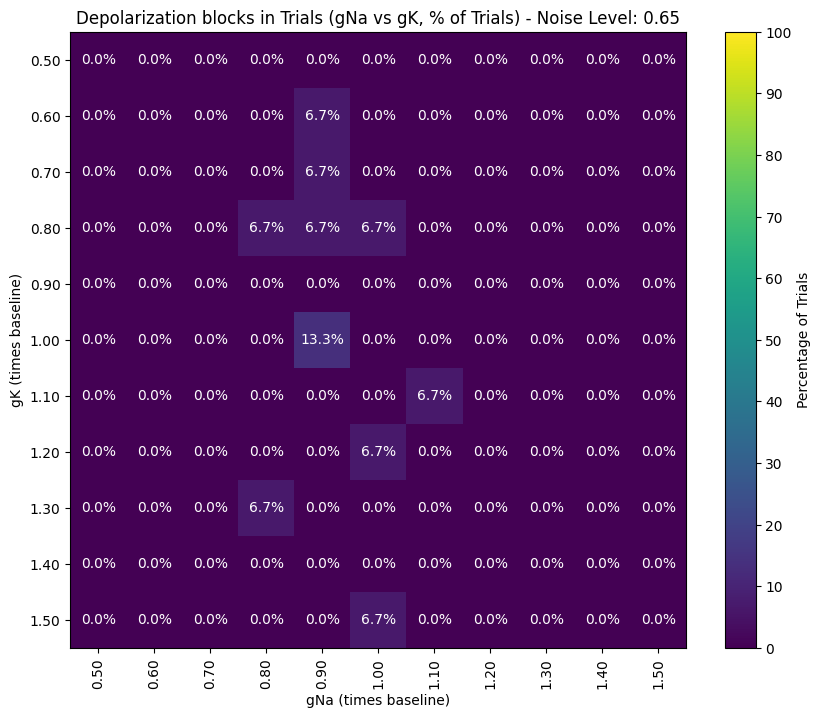
\includegraphics[width=\linewidth]{DPB_percentage_matrices/DPB_percentage_noise_0.65.png}
        \caption{} % Optional caption
    \end{subfigure}\hfill
    \begin{subfigure}{0.48\textwidth}
        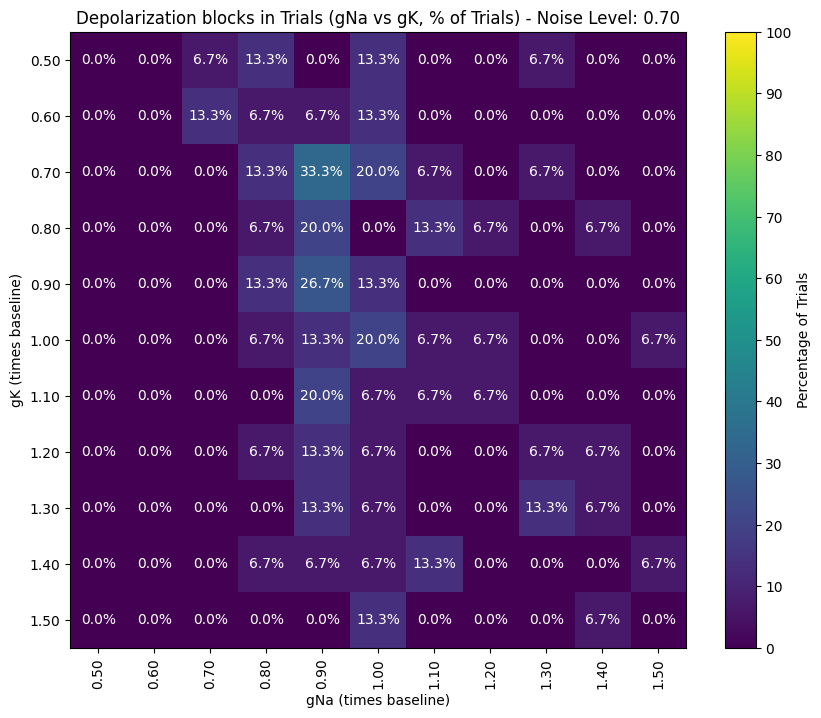
\includegraphics[width=\linewidth]{DPB_percentage_matrices/DPB_percentage_noise_0.70.png}
        \caption{} % Optional caption
    \end{subfigure}

    \bigskip % Adds vertical space between the rows

    % Row 2
    \begin{subfigure}{0.48\textwidth}
        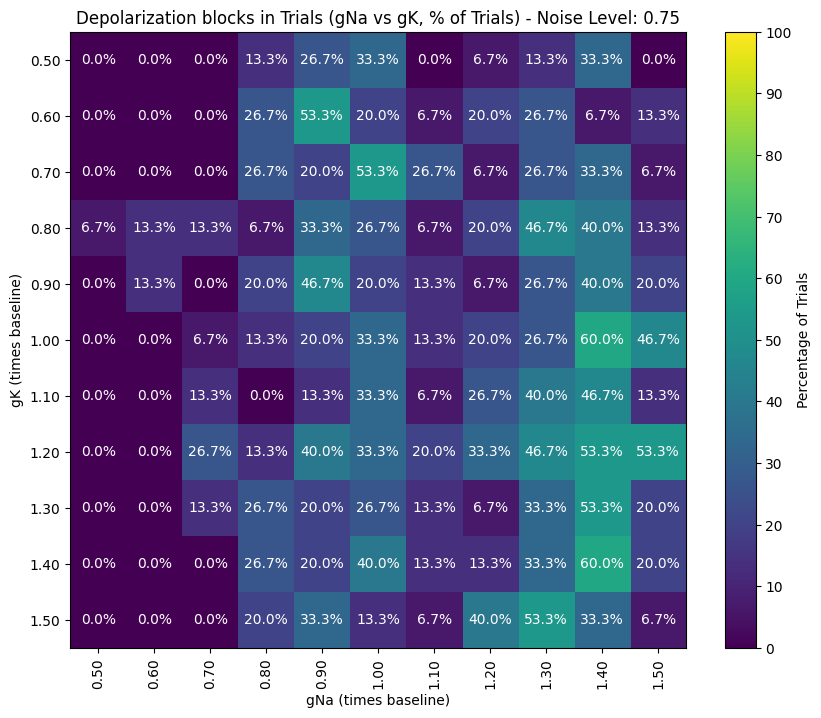
\includegraphics[width=\linewidth]{DPB_percentage_matrices/DPB_percentage_noise_0.75.png}
        \caption{} % Optional caption
    \end{subfigure}\hfill
    \begin{subfigure}{0.48\textwidth}
        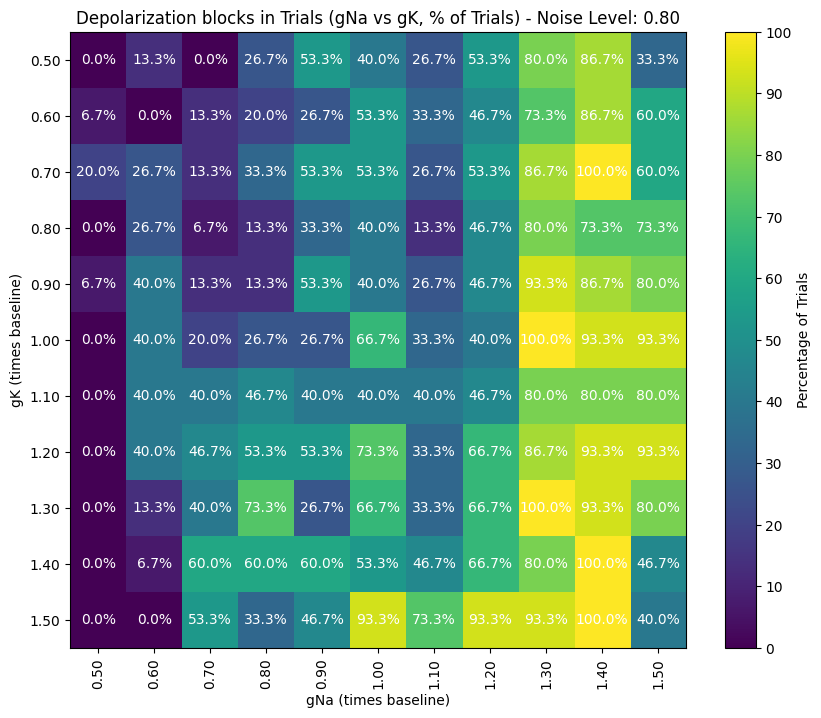
\includegraphics[width=\linewidth]{DPB_percentage_matrices/DPB_percentage_noise_0.80.png}
        \caption{} % Optional caption
    \end{subfigure}

    \caption[DPB percentage matrices (all)]{Percentage of trials where depolarization block events occurred for all tested noise conditions.
        The x-axis shows all the sodium conductance changes in pyramidal cells, whereas the y-axis shows the potassium conductance changes in pyramidal cells.
        Modifications to pyramidal cells were applied to all compartments.
        The color intensity scales from 0 to 100 \%, where high-intensity yellow equals a higher amount of DPB events in a condition.
        The images are labeled from low noise to higher noise (a through k), respectively.}\label{fig:dpb_percentage_matrices_all}
\end{figure}

% Page 2
\begin{figure}[H] \ContinuedFloat
    \centering
    % Row 3
    \begin{subfigure}{0.48\textwidth}
        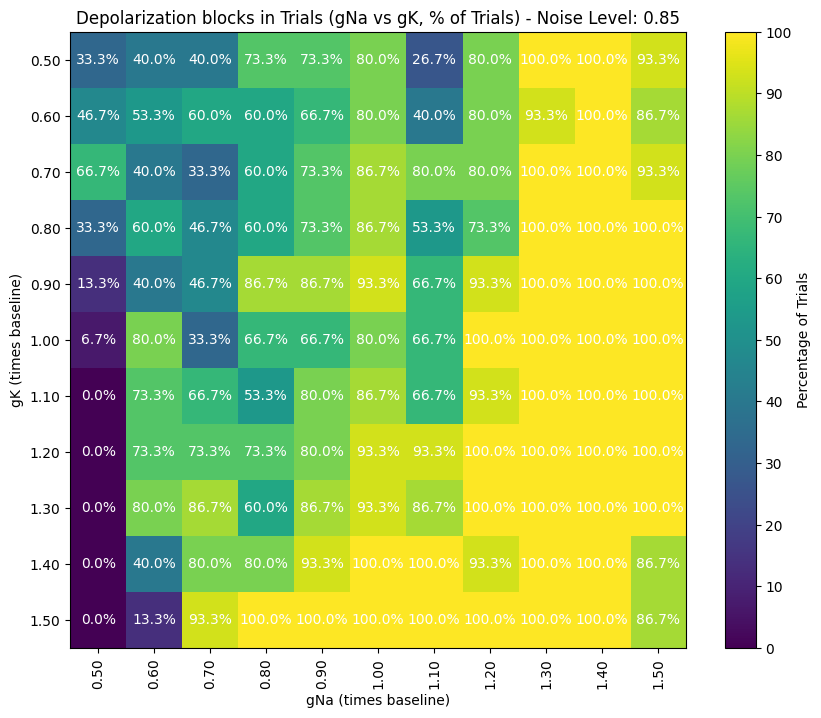
\includegraphics[width=\linewidth]{DPB_percentage_matrices/DPB_percentage_noise_0.85.png}
        \caption{} % Optional caption
    \end{subfigure}\hfill
    \begin{subfigure}{0.48\textwidth}
        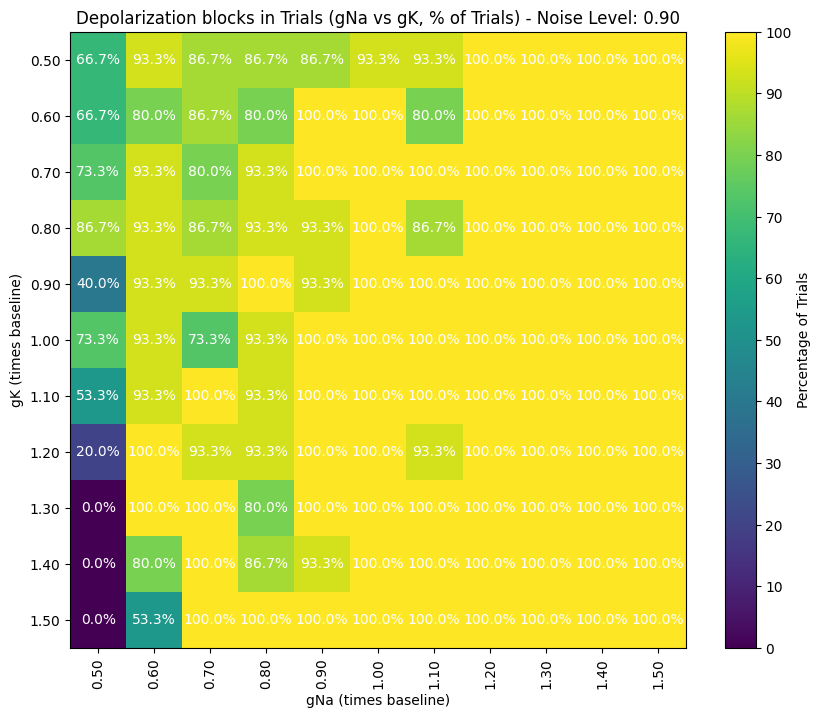
\includegraphics[width=\linewidth]{DPB_percentage_matrices/DPB_percentage_noise_0.90.png}
        \caption{} % Optional caption
    \end{subfigure}

    \bigskip % Adds vertical space between the rows

    % Row 4
    \begin{subfigure}{0.48\textwidth}
        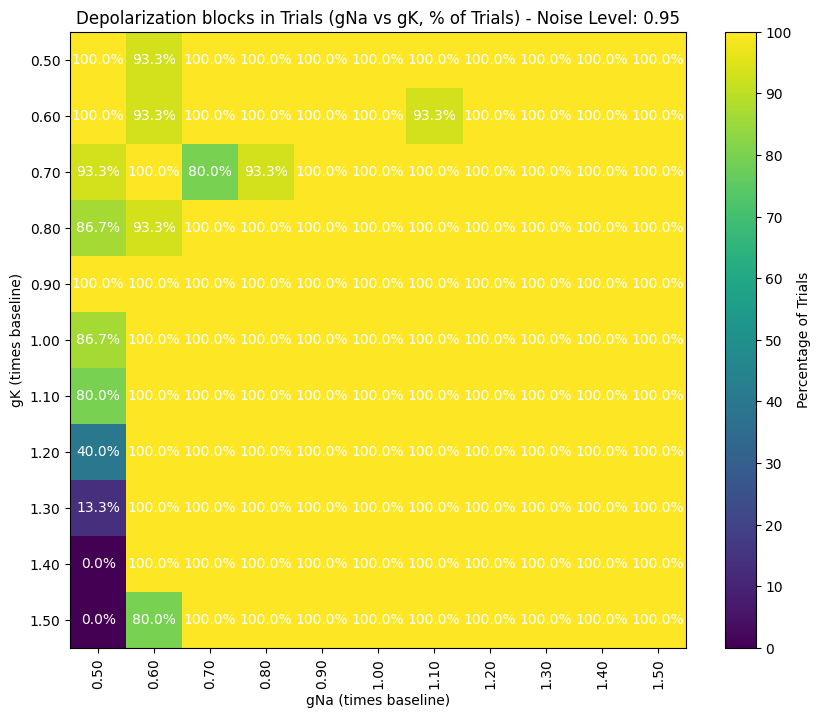
\includegraphics[width=\linewidth]{DPB_percentage_matrices/DPB_percentage_noise_0.95.png}
        \caption{} % Optional caption
    \end{subfigure}\hfill
    \begin{subfigure}{0.48\textwidth}
        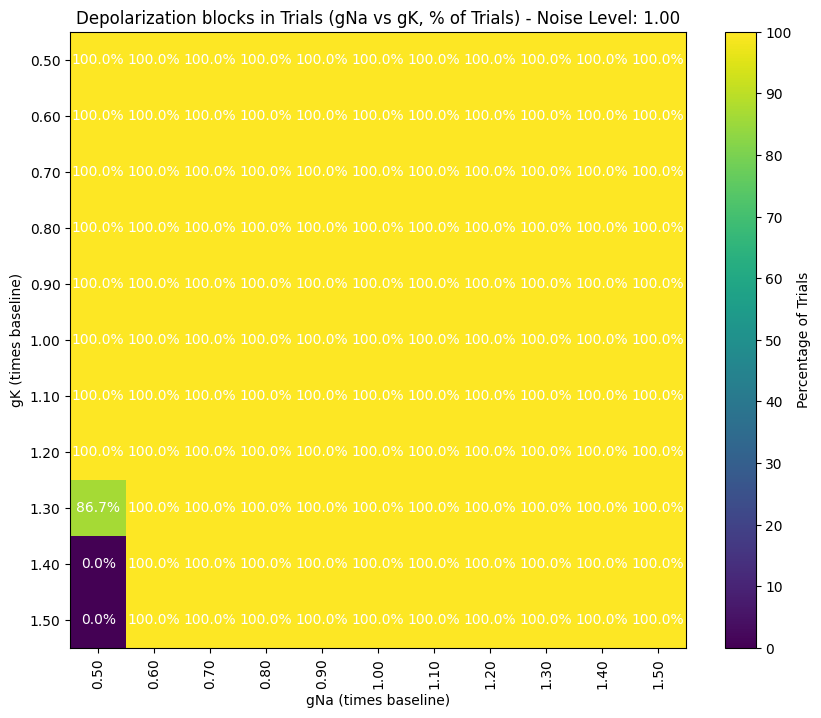
\includegraphics[width=\linewidth]{DPB_percentage_matrices/DPB_percentage_noise_1.00.png}
        \caption{} % Optional caption
    \end{subfigure}
\end{figure}

% Page 3
\begin{figure}[H] \ContinuedFloat
    \centering
    % Row 5
    \begin{subfigure}{0.48\textwidth}
        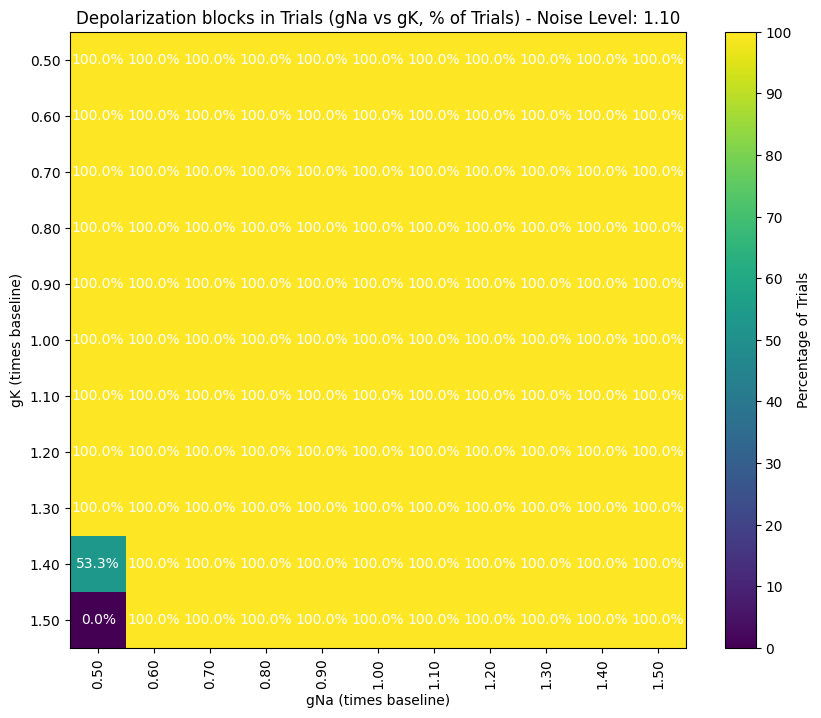
\includegraphics[width=\linewidth]{DPB_percentage_matrices/DPB_percentage_noise_1.10.png}
        \caption{} % Optional caption
    \end{subfigure}\hfill
    \begin{subfigure}{0.48\textwidth}
        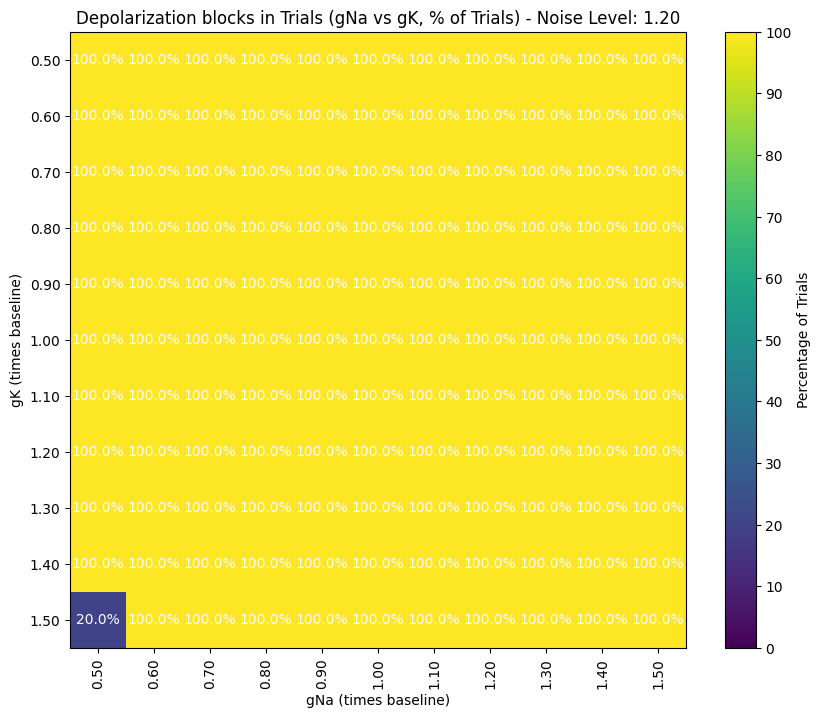
\includegraphics[width=\linewidth]{DPB_percentage_matrices/DPB_percentage_noise_1.20.png}
        \caption{} % Optional caption
    \end{subfigure}

    \bigskip % Adds vertical space between the rows

    % Row 6
    \begin{subfigure}{0.48\textwidth}
        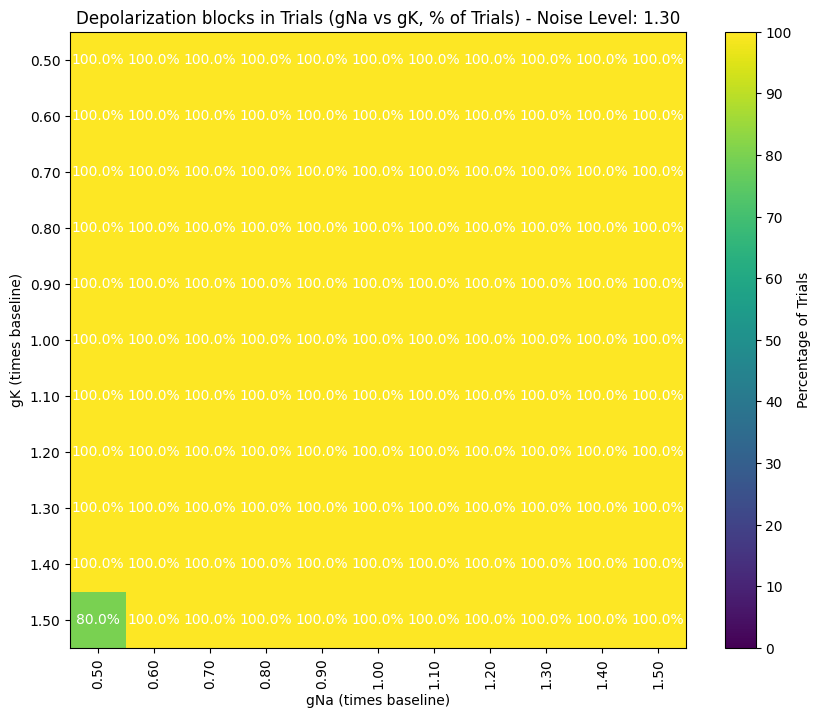
\includegraphics[width=\linewidth]{DPB_percentage_matrices/DPB_percentage_noise_1.30.png}
        \caption{} % Optional caption
    \end{subfigure}
    % Since the last row has only one image, you might adjust its position or add another sub-figure if needed.
\end{figure}
\pagebreak

\subsection{External Noise variants: DPB delay matrices}\label{subsec:DPB_delay_matrices}
% Page 1
\begin{figure}[H]
    \centering
    % Row 1
    \begin{subfigure}{0.48\textwidth}
        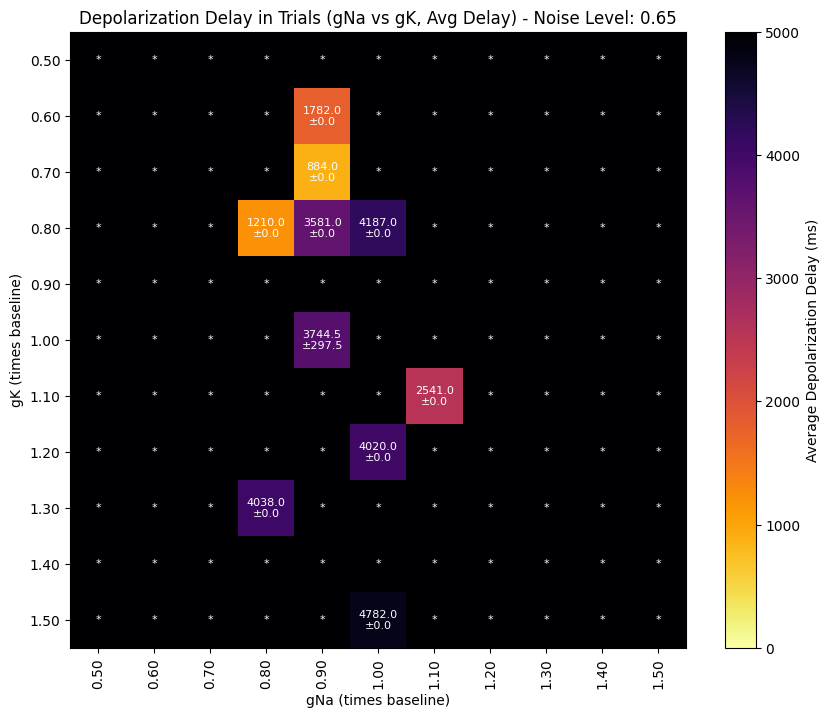
\includegraphics[width=\linewidth]{DPB_delay_matrices/DPB_delay_noise_0.65.png}
        \caption{} % Optional caption
    \end{subfigure}\hfill
    \begin{subfigure}{0.48\textwidth}
        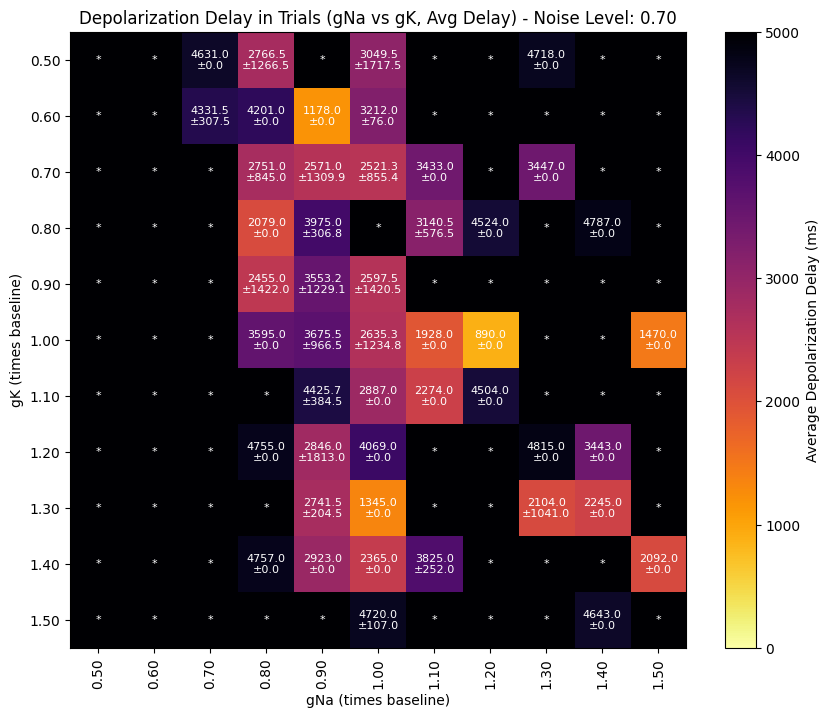
\includegraphics[width=\linewidth]{DPB_delay_matrices/DPB_delay_noise_0.70.png}
        \caption{} % Optional caption
    \end{subfigure}

    \bigskip % Adds vertical space between the rows

    % Row 2
    \begin{subfigure}{0.48\textwidth}
        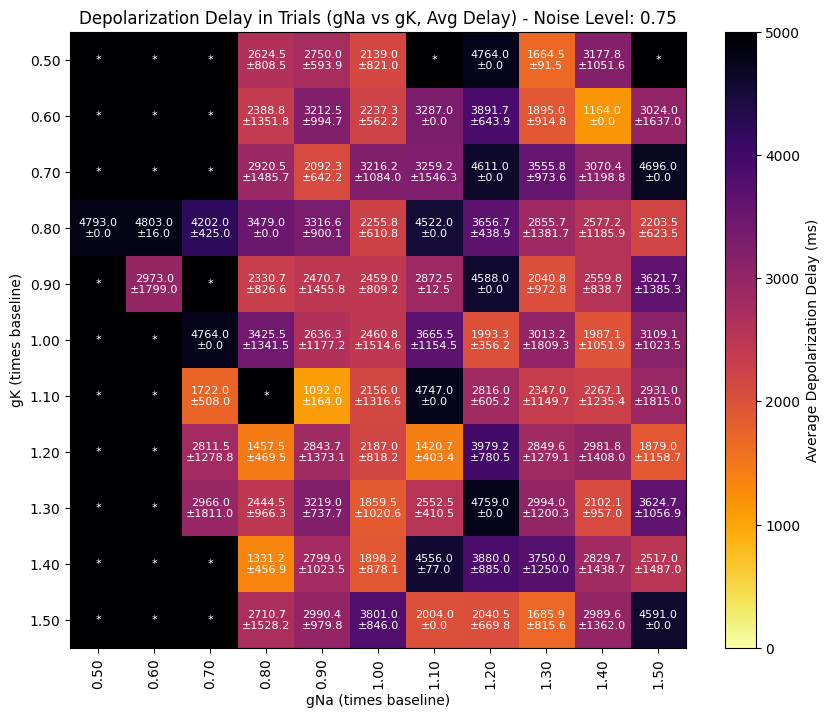
\includegraphics[width=\linewidth]{DPB_delay_matrices/DPB_delay_noise_0.75.png}
        \caption{} % Optional caption
    \end{subfigure}\hfill
    \begin{subfigure}{0.48\textwidth}
        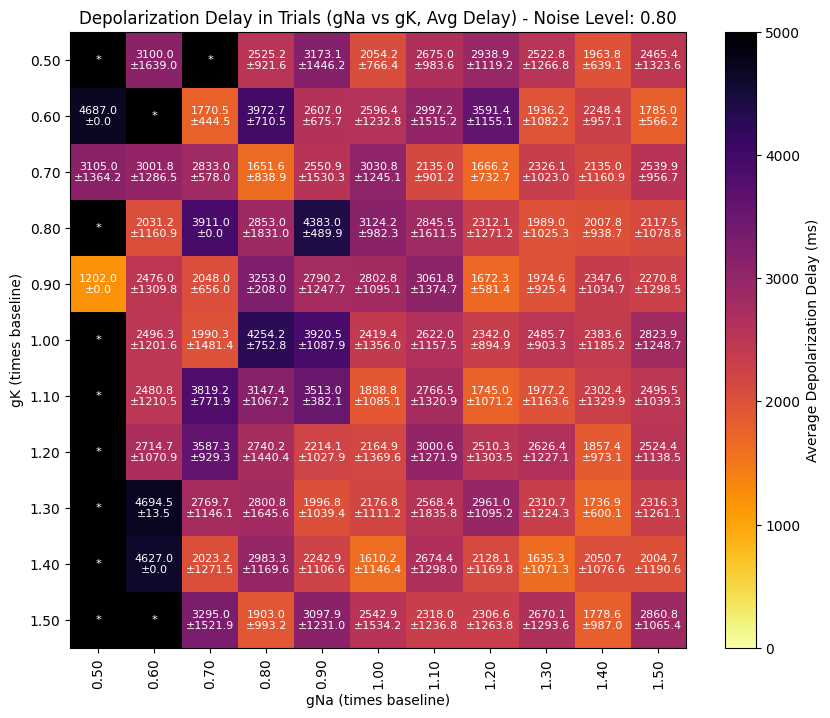
\includegraphics[width=\linewidth]{DPB_delay_matrices/DPB_delay_noise_0.80.png}
        \caption{} % Optional caption
    \end{subfigure}

    \caption[DPB delay matrices (all)]{Average delay + Standard deviation of DPB in trials where depolarization block events occurred for all tested noise conditions.
        The x-axis shows all the sodium conductance changes in pyramidal cells, whereas the y-axis shows the potassium conductance changes in pyramidal cells.
        Modifications to pyramidal cells were applied to all compartments.
        The color intensity shows the average delay, where high-intensity red equals a shorter delay in DPB events in a condition.
        The images are labeled from low noise to higher noise (a through k), respectively.}\label{fig:dpb_delay_matrices_all}
\end{figure}

% Page 2
\begin{figure}[H] \ContinuedFloat
    \centering
    % Row 3
    \begin{subfigure}{0.48\textwidth}
        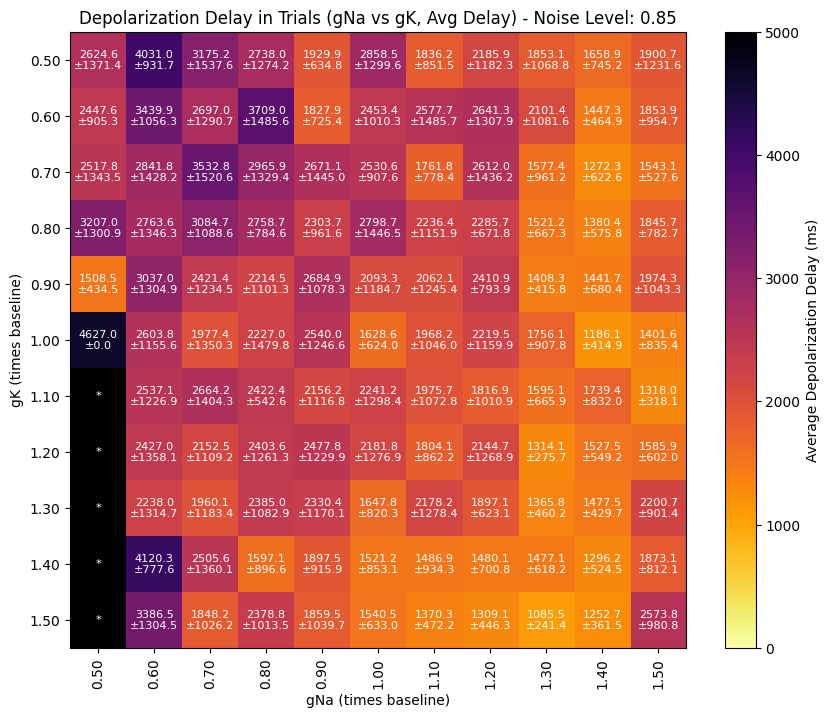
\includegraphics[width=\linewidth]{DPB_delay_matrices/DPB_delay_noise_0.85.png}
        \caption{} % Optional caption
    \end{subfigure}\hfill
    \begin{subfigure}{0.48\textwidth}
        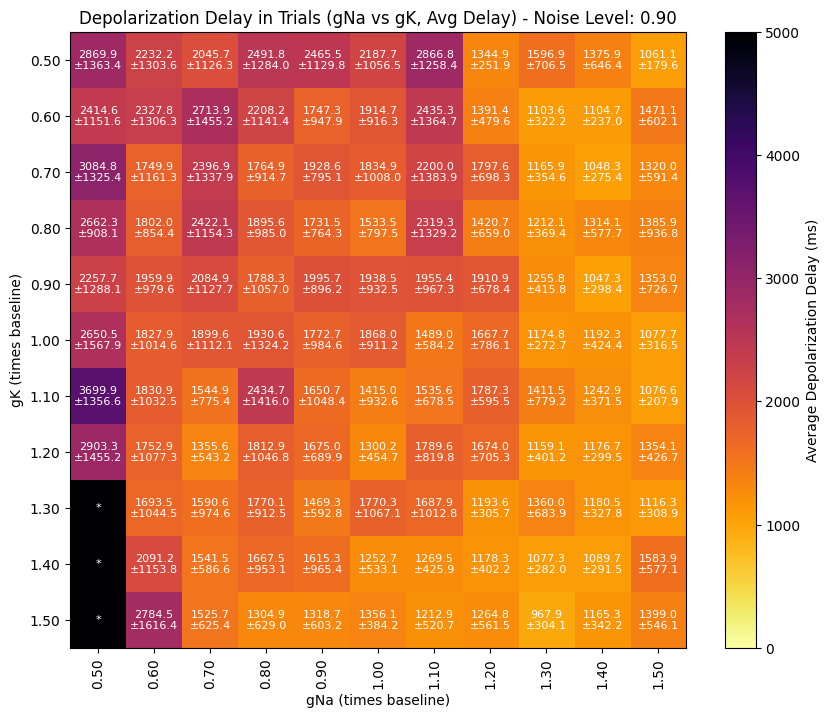
\includegraphics[width=\linewidth]{DPB_delay_matrices/DPB_delay_noise_0.90.png}
        \caption{} % Optional caption
    \end{subfigure}

    \bigskip % Adds vertical space between the rows

    % Row 4
    \begin{subfigure}{0.48\textwidth}
        \includegraphics[width=\linewidth]{DPB_delay_matrices/DPB_delay_noise_0.95.png}
        \caption{} % Optional caption
    \end{subfigure}\hfill
    \begin{subfigure}{0.48\textwidth}
        \includegraphics[width=\linewidth]{DPB_delay_matrices/DPB_delay_noise_1.00.png}
        \caption{} % Optional caption
    \end{subfigure}
\end{figure}

% Page 3
\begin{figure}[H] \ContinuedFloat
    \centering
    % Row 5
    \begin{subfigure}{0.48\textwidth}
        \includegraphics[width=\linewidth]{DPB_delay_matrices/DPB_delay_noise_1.10.png}
        \caption{} % Optional caption
    \end{subfigure}\hfill
    \begin{subfigure}{0.48\textwidth}
        \includegraphics[width=\linewidth]{DPB_delay_matrices/DPB_delay_noise_1.20.png}
        \caption{} % Optional caption
    \end{subfigure}

    \bigskip % Adds vertical space between the rows

    % Row 6
    \begin{subfigure}{0.48\textwidth}
        \includegraphics[width=\linewidth]{DPB_delay_matrices/DPB_delay_noise_1.30.png}
        \caption{} % Optional caption
    \end{subfigure}
    % Since the last row has only one image, you might adjust its position or add another sub-figure if needed.
\end{figure}
\pagebreak

\subsection{Recurrent connection matrices}\label{subsec:recurrent_connection_matrices}
% Page 1
\begin{figure}[H]
    \centering
    % Row 1
    \begin{subfigure}{0.48\textwidth}
        \includegraphics[width=\linewidth]{DPB_RC_Percentages/DPB_percentages_RC_1.00.png}
        \caption{} % Optional caption
    \end{subfigure}\hfill
    \begin{subfigure}{0.48\textwidth}
        \includegraphics[width=\linewidth]{DPB_RC_Percentages/DPB_percentages_RC_1.05.png}
        \caption{} % Optional caption
    \end{subfigure}

    \bigskip % Adds vertical space between the rows

    % Row 2
    \begin{subfigure}{0.48\textwidth}
        \includegraphics[width=\linewidth]{DPB_RC_Percentages/DPB_percentages_RC_1.10.png}
        \caption{} % Optional caption
    \end{subfigure}\hfill
    \begin{subfigure}{0.48\textwidth}
        \includegraphics[width=\linewidth]{DPB_RC_Percentages/DPB_percentages_RC_1.15.png}
        \caption{} % Optional caption
    \end{subfigure}

    \caption[RC DPB percentage matrices (all)]{Percentage of trials where depolarization block events occurred for all tested noise conditions.
        The x-axis shows all the sodium conductance changes in pyramidal cells, whereas the y-axis shows the potassium conductance changes in pyramidal cells.
        Modifications to pyramidal cells were applied to all compartments.
        The color intensity shows the average delay, where high-intensity yellow equals higher percentage of DPB events in a condition.
        The images are labeled from low noise to higher noise (a through e), respectively.}\label{fig:rc_dpb_percentage_matrices_all}
\end{figure}

% Page 2
\begin{figure}[H] \ContinuedFloat
    \centering
    % Row 3
    \begin{subfigure}{0.48\textwidth}
        \includegraphics[width=\linewidth]{DPB_RC_Percentages/DPB_percentages_RC_1.20.png}
        \caption{} % Optional caption
    \end{subfigure}\hfill
\end{figure}

\end{document}